% Options for packages loaded elsewhere
\PassOptionsToPackage{unicode}{hyperref}
\PassOptionsToPackage{hyphens}{url}
\documentclass[
  11pt]{article}
\usepackage{xcolor}
\usepackage[margin=1in]{geometry}
\usepackage{amsmath,amssymb}
\setcounter{secnumdepth}{-\maxdimen} % remove section numbering
\usepackage{iftex}
\ifPDFTeX
  \usepackage[T1]{fontenc}
  \usepackage[utf8]{inputenc}
  \usepackage{textcomp} % provide euro and other symbols
\else % if luatex or xetex
  \usepackage{unicode-math} % this also loads fontspec
  \defaultfontfeatures{Scale=MatchLowercase}
  \defaultfontfeatures[\rmfamily]{Ligatures=TeX,Scale=1}
\fi
\usepackage{lmodern}
\ifPDFTeX\else
  % xetex/luatex font selection
\fi
% Use upquote if available, for straight quotes in verbatim environments
\IfFileExists{upquote.sty}{\usepackage{upquote}}{}
\IfFileExists{microtype.sty}{% use microtype if available
  \usepackage[]{microtype}
  \UseMicrotypeSet[protrusion]{basicmath} % disable protrusion for tt fonts
}{}
\makeatletter
\@ifundefined{KOMAClassName}{% if non-KOMA class
  \IfFileExists{parskip.sty}{%
    \usepackage{parskip}
  }{% else
    \setlength{\parindent}{0pt}
    \setlength{\parskip}{6pt plus 2pt minus 1pt}}
}{% if KOMA class
  \KOMAoptions{parskip=half}}
\makeatother
\usepackage{longtable,booktabs,array}
\newcounter{none} % for unnumbered tables
\usepackage{calc} % for calculating minipage widths
% Correct order of tables after \paragraph or \subparagraph
\usepackage{etoolbox}
\makeatletter
\patchcmd\longtable{\par}{\if@noskipsec\mbox{}\fi\par}{}{}
\makeatother
% Allow footnotes in longtable head/foot
\IfFileExists{footnotehyper.sty}{\usepackage{footnotehyper}}{\usepackage{footnote}}
\makesavenoteenv{longtable}
\usepackage{graphicx}
\makeatletter
\newsavebox\pandoc@box
\newcommand*\pandocbounded[1]{% scales image to fit in text height/width
  \sbox\pandoc@box{#1}%
  \Gscale@div\@tempa{\textheight}{\dimexpr\ht\pandoc@box+\dp\pandoc@box\relax}%
  \Gscale@div\@tempb{\linewidth}{\wd\pandoc@box}%
  \ifdim\@tempb\p@<\@tempa\p@\let\@tempa\@tempb\fi% select the smaller of both
  \ifdim\@tempa\p@<\p@\scalebox{\@tempa}{\usebox\pandoc@box}%
  \else\usebox{\pandoc@box}%
  \fi%
}
% Set default figure placement to htbp
\def\fps@figure{htbp}
\makeatother
\setlength{\emergencystretch}{3em} % prevent overfull lines
\providecommand{\tightlist}{%
  \setlength{\itemsep}{0pt}\setlength{\parskip}{0pt}}
% LaTeX preamble for REPORT.md, inserted by pandoc (see ../build.sh).
\usepackage{etoolbox}
\usepackage{libertinus-otf}          % Libertinus text and math, with Greek and minus signs
\usepackage{microtype}
\usepackage{booktabs}
\usepackage{caption}
\captionsetup{font=small,labelfont=bf,skip=4pt}
\captionsetup[figure]{labelformat=empty} % the figure number is written in the caption text
\usepackage{float}
\usepackage{xcolor}
\definecolor{linkblue}{HTML}{1F4E79}
\AtBeginDocument{\hypersetup{colorlinks=true,linkcolor=linkblue,urlcolor=linkblue,citecolor=linkblue}}
\usepackage{fancyhdr}
\pagestyle{fancy}
\fancyhf{}
\fancyhead[L]{\small\itshape Model-Free Q-Learning and Optimal Portfolio Choice}
\fancyhead[R]{\small\itshape Aldrich and Harkless}
\fancyfoot[C]{\small\thepage}
\renewcommand{\headrulewidth}{0.4pt}
\setlength{\headheight}{14pt}
\usepackage{titlesec}
\titleformat{\section}{\large\bfseries}{}{0pt}{}
\titleformat{\subsection}{\normalsize\bfseries}{}{0pt}{}
\titlespacing*{\section}{0pt}{14pt plus 3pt minus 2pt}{6pt}
\titlespacing*{\subsection}{0pt}{10pt plus 2pt minus 2pt}{4pt}
% Tables: smaller type and tighter rows so the wide ones fit the text width.
\AtBeginEnvironment{longtable}{\small\renewcommand{\arraystretch}{1.1}}
\setlength{\LTpre}{6pt}\setlength{\LTpost}{6pt}
% Figures and tables float to the top or bottom of the page, LaTeX style.
\makeatletter\def\fps@figure{htbp}\makeatother
\setlength{\parskip}{4pt plus 1pt}
\setlength{\parindent}{0pt}
\AtBeginEnvironment{verbatim}{\footnotesize}
\AtBeginEnvironment{Shaded}{\footnotesize}
% Figure paths in REPORT.md are relative to docs/report/.
\graphicspath{{../}}
\captionsetup[table]{labelformat=empty,position=top}
\renewcommand{\topfraction}{0.85}\renewcommand{\bottomfraction}{0.6}\renewcommand{\textfraction}{0.12}\renewcommand{\floatpagefraction}{0.75}
\usepackage{bookmark}
\IfFileExists{xurl.sty}{\usepackage{xurl}}{} % add URL line breaks if available
\urlstyle{same}
\hypersetup{
  pdftitle={Model-Free Q-Learning and Optimal Portfolio Choice with Nine Assets},
  pdfauthor={Albert Aldrich and William Harkless},
  hidelinks,
  pdfcreator={LaTeX via pandoc}}

\title{Model-Free Q-Learning and Optimal Portfolio Choice with Nine
Assets}
\author{Albert Aldrich and William Harkless}
\date{Data Science for Finance, Fall 2026}

\begin{document}
\maketitle

\subsection{Abstract}\label{abstract}

We ask whether a model-free learner can recover a near-optimal
mean-variance portfolio from realized rewards alone. Nine ETFs are
calibrated on 5,152 daily excess returns (February 2006 to July 2026),
the estimated moments become the fixed truth of a Gaussian simulator,
and a stateless tabular Q-learning agent chooses among the 1,287
long-only portfolios on a 20\% weight grid. At risk aversion γ = 5,
across ten seeds, the median learned portfolio is 14.1 bps/yr of
certainty-equivalent return behind the best grid portfolio and 19.8
behind the continuous optimum, which is worth 530.5; equal weighting is
310.9 behind. Three seeds of ten find the best grid portfolio exactly.
Exact recovery fails because the two best grid portfolios differ by 10.5
bps/yr while one 20-day episode's reward has a standard deviation near
3,900. A finer grid trades discretization error for learning error and
does not lower the total gap at this budget. Two post hoc extensions are
reported with their failures. Spline function approximation beats a
constant-step table on the 20\% grid at two of three risk aversions and
loses to the \(1/N\) table on the 10\% grid, in a comparison that also
changes the step-size rule. With transaction costs and drifting
holdings, the agent trails a full-information oracle by 13.1 bps/yr at
zero cost and 2.8 at \$10 billion. Its trade timing is worth 6.2 bps/yr
there, but most of the narrowing comes from a target closer to the best
one, which we have not explained. Only the four baseline experiments
were specified before any full-scale run.

\subsection{1. Introduction and central research
question}\label{introduction-and-central-research-question}

Can a model-free learning algorithm recover a near-optimal portfolio
allocation when it observes realized rewards but does not know expected
returns or covariances? We study the question in a controlled
experiment. A mean vector μ and covariance matrix Σ are estimated once
from nine ETFs and then treated as the truth of a synthetic market. The
agent never sees them. It picks a portfolio, holds it for a short
episode of simulated returns, receives the realized mean-variance
reward, and updates one value per portfolio.

Three portfolios define the gaps we report. The continuous optimum
\(w^*\) is the best long-only, fully invested portfolio; the best grid
portfolio is the best one the agent may choose; the learned portfolio is
the one it chose. The discretization gap is the best grid portfolio's
loss against \(w^*\), the learning gap is the learned portfolio's loss
against the best grid portfolio, and their sum is the total gap. Each
gap is a certainty-equivalent loss, \(252 \times 10^4 \times \Delta U\)
in bps/yr with \(U\) daily mean-variance utility, so it reads as the
sure annual return the investor gives up. Section 3 separates the
continuous optimum from the best grid portfolio and Section 5 separates
learning from discretization error. Calibration uses historical data
once, and evaluation uses simulated draws that never updated a Q-value
(Section 2). Section 5 reports statistical convergence (the agent's
table stops changing) beside economic convergence (its choice stays
within 25 bps/yr of the best available).

Only the four baseline experiments (γ = 5 on the 20\% and 25\% grids, γ
= 3 and γ = 8 on the 20\% grid) had their settings and convergence rules
fixed before any full-scale run. Every other run is labeled post hoc
wherever it appears.

\subsection{2. ETF data, sample construction, and
calibration}\label{etf-data-sample-construction-and-calibration}

\textbf{Universe and sources.} The nine ETFs are SPY, EFA and EEM
(equity), IEF, LQD and TIP (fixed income), and GLD, VNQ and DBC (real
assets). Daily prices come from Yahoo Finance through \texttt{yfinance}
1.7.0 and the daily risk-free rate from the Kenneth French Data Library.
The environment is defined on excess returns.

\textbf{Returns and adjustment.} Returns are simple returns on the
Adjusted Close, \(r_t = P_t / P_{t-1} - 1\); no log returns are used. We
verified the adjustment convention two ways: Adjusted Close and Close
differ only on distribution dates, by the amount the distribution
implies (worst discrepancy \(6.0 \times 10^{-4}\)), and EEM's
three-for-one split of 24 July 2008 leaves no jump in the returns.

\textbf{Sample.} The sample runs from 7 February 2006, the day after
DBC's first price in the data, to 31 July 2026, where the risk-free file
ends (we truncated rather than forward-fill the rate), for 5,152 daily
observations. Dates are aligned by an inner join across the nine ETFs.
The 5,214 raw SPY rows lose 23 dates before DBC's inception, 36 after
the risk-free file ends, one incomplete final session, one date missing
at the vendor and one row to differencing. Extreme days such as EEM's
+22.77\% on 13 October 2008 are kept.

\textbf{One frequency.} μ, Σ, risk aversion and all rewards are daily.
Annualization (×252 for means and utilities, ×√252 for volatilities) is
for reporting only.

\begin{table}[htbp]
\centering\small
\caption{\textbf{Table 1.} Annualized summary statistics of daily excess
returns, 7 February 2006 to 31 July 2026. SE is the standard error of
the annualized mean; kurtosis is excess kurtosis.}
\begin{tabular}{@{}
  >{\raggedright\arraybackslash}p{(\linewidth - 12\tabcolsep) * \real{0.0638}}
  >{\raggedright\arraybackslash}p{(\linewidth - 12\tabcolsep) * \real{0.3191}}
  >{\raggedleft\arraybackslash}p{(\linewidth - 12\tabcolsep) * \real{0.1170}}
  >{\raggedleft\arraybackslash}p{(\linewidth - 12\tabcolsep) * \real{0.1383}}
  >{\raggedleft\arraybackslash}p{(\linewidth - 12\tabcolsep) * \real{0.1383}}
  >{\raggedleft\arraybackslash}p{(\linewidth - 12\tabcolsep) * \real{0.0957}}
  >{\raggedleft\arraybackslash}p{(\linewidth - 12\tabcolsep) * \real{0.1277}}@{}}
\toprule\noalign{}
\begin{minipage}[b]{\linewidth}\raggedright
ETF
\end{minipage} & \begin{minipage}[b]{\linewidth}\raggedright
Exposure
\end{minipage} & \begin{minipage}[b]{\linewidth}\raggedleft
Mean (\%)
\end{minipage} & \begin{minipage}[b]{\linewidth}\raggedleft
SE (\%)
\end{minipage} & \begin{minipage}[b]{\linewidth}\raggedleft
Vol. (\%)
\end{minipage} & \begin{minipage}[b]{\linewidth}\raggedleft
Sharpe
\end{minipage} & \begin{minipage}[b]{\linewidth}\raggedleft
Kurtosis
\end{minipage} \\
\midrule\noalign{}
SPY & U.S. large-cap stocks & 10.7 & 4.27 & 19.3 & 0.55 & 15.0 \\
EFA & Developed markets ex U.S. & 6.1 & 4.73 & 21.4 & 0.29 & 13.9 \\
EEM & Emerging-market stocks & 7.5 & 6.20 & 28.0 & 0.27 & 17.8 \\
IEF & 7 to 10 year Treasuries & 1.7 & 1.51 & 6.8 & 0.25 & 2.7 \\
LQD & Investment-grade corporates & 2.6 & 1.91 & 8.6 & 0.30 & 58.9 \\
TIP & Inflation-protected Treasuries & 1.7 & 1.37 & 6.2 & 0.28 & 10.2 \\
GLD & Gold bullion & 9.2 & 4.08 & 18.4 & 0.50 & 6.5 \\
VNQ & U.S. REITs & 8.9 & 6.42 & 29.0 & 0.31 & 17.2 \\
DBC & Broad commodity futures & 2.3 & 4.27 & 19.3 & 0.12 & 3.0 \\
\bottomrule\noalign{}
\end{tabular}
\end{table}

Figure A1 gives the correlation matrix. SPY and GLD have the two highest
Sharpe ratios (0.55 and 0.50) and a correlation of 0.07, and IEF is
negatively correlated with SPY (−0.29), which anticipates the optimum in
Section 3. The three equity funds are close substitutes (correlations
0.82 to 0.88), as are IEF and TIP (0.76).

\textbf{Ground-truth environment.} The simulator draws
\(r_{t+1} = \mu + L z_{t+1}\) with \(z \sim \mathcal{N}(0, I_9)\) and
\(L\) the Cholesky factor of Σ, so returns are independent
\(\mathcal{N}(\mu, \Sigma)\) draws. The moments are the truth inside the
experiment only. Training returns, exploration draws and evaluation
returns come from separate random streams of one master seed, so
evaluation never reuses training data and seed \(i\) sees the same
returns in every comparable run.

\textbf{Leakage guard.} The agent receives only its action index and a
scalar reward. Unit tests stop its code from importing the data loader,
the benchmark module or the data files.

\subsection{3. Theoretical benchmark and feasible portfolio
set}\label{theoretical-benchmark-and-feasible-portfolio-set}

\textbf{Objective.} The investor maximizes daily mean-variance utility

\[U(w) = w^\top \mu - \frac{\gamma}{2}\, w^\top \Sigma\, w .\]

The baseline is γ = 5, with γ = 3 and γ = 8 as robustness values. γ = 5
lies inside the range of 2 to 7 that the meta-analysis of Elminejad,
Havranek and Irsova (2025) reports for the finance literature, is
consistent with the household survey of Barsky et al.~(1997), in which
most respondents fall in the least risk-tolerant category, and is well
under the bound of 10 that Mehra and Prescott (1985) regard as
plausible. We rejected the value the data imply (2.9) so that the data
would not choose their own risk aversion.

\textbf{Budget-only closed form.} With only \(\mathbf{1}^\top w = 1\),
the first-order condition of
\(\mathcal{L} = w^\top\mu - \tfrac{\gamma}{2} w^\top \Sigma w - \eta(\mathbf{1}^\top w - 1)\)
is \(\mu - \gamma \Sigma w - \eta \mathbf{1} = 0\), and the budget
constraint fixes the multiplier:

\[w_{\text{budget}} = \frac{1}{\gamma}\,\Sigma^{-1}\left(\mu - \eta\,\mathbf{1}\right), \qquad \eta = \frac{\mathbf{1}^\top \Sigma^{-1}\mu - \gamma}{\mathbf{1}^\top \Sigma^{-1}\mathbf{1}} .\]

Our implementation agrees with an independent numerical solve to within
\(1.5 \times 10^{-6}\) (Appendix B). The portfolio takes short
positions, so it lies outside the agent's feasible set and is not the
benchmark for the learning comparison.

\textbf{Feasible set and the two benchmarks.} The agent's feasible set
is long-only and fully invested (\(w_i \ge 0\), \(\sum_i w_i = 1\)), and
the benchmark is solved numerically under the same constraints. For
every specification we report two benchmarks: the continuous optimum
\(w^*\), which maximizes \(U\) over the simplex, and the best grid
portfolio, found by evaluating every action.

\textbf{Action set.} An action is nine weights in multiples of a step
\(h\) that sum to one, generated from the asset count and \(h\) alone;
no moment enters and the optimum is not inserted. There are 495
portfolios at \(h\) = 25\%, 1,287 at 20\% (the baseline), 43,758 at 10\%
and 3,108,105 at 5\% (counted only).

\begin{table}[htbp]
\centering\small
\caption{\textbf{Table 2.} Continuous long-only optimum \(w^*\) and best
20\% grid portfolio, weights in percent; the other six ETFs are zero in
every row. Return and volatility (Vol.) are annualized; \(U(w^*)\) and
the discretization gap are in bps/yr.}
\begin{tabular}{@{}
  >{\raggedright\arraybackslash}p{(\linewidth - 20\tabcolsep) * \real{0.0366}}
  >{\raggedleft\arraybackslash}p{(\linewidth - 20\tabcolsep) * \real{0.1098}}
  >{\raggedleft\arraybackslash}p{(\linewidth - 20\tabcolsep) * \real{0.1098}}
  >{\raggedleft\arraybackslash}p{(\linewidth - 20\tabcolsep) * \real{0.1098}}
  >{\raggedleft\arraybackslash}p{(\linewidth - 20\tabcolsep) * \real{0.0976}}
  >{\raggedleft\arraybackslash}p{(\linewidth - 20\tabcolsep) * \real{0.1098}}
  >{\raggedleft\arraybackslash}p{(\linewidth - 20\tabcolsep) * \real{0.1098}}
  >{\raggedleft\arraybackslash}p{(\linewidth - 20\tabcolsep) * \real{0.0732}}
  >{\raggedleft\arraybackslash}p{(\linewidth - 20\tabcolsep) * \real{0.0732}}
  >{\raggedleft\arraybackslash}p{(\linewidth - 20\tabcolsep) * \real{0.0732}}
  >{\raggedleft\arraybackslash}p{(\linewidth - 20\tabcolsep) * \real{0.0976}}@{}}
\toprule\noalign{}
\begin{minipage}[b]{\linewidth}\raggedright
γ
\end{minipage} & \begin{minipage}[b]{\linewidth}\raggedleft
\(w^*\) SPY
\end{minipage} & \begin{minipage}[b]{\linewidth}\raggedleft
\(w^*\) IEF
\end{minipage} & \begin{minipage}[b]{\linewidth}\raggedleft
\(w^*\) GLD
\end{minipage} & \begin{minipage}[b]{\linewidth}\raggedleft
Return
\end{minipage} & \begin{minipage}[b]{\linewidth}\raggedleft
Vol.
\end{minipage} & \begin{minipage}[b]{\linewidth}\raggedleft
\(U(w^*)\)
\end{minipage} & \begin{minipage}[b]{\linewidth}\raggedleft
Grid SPY
\end{minipage} & \begin{minipage}[b]{\linewidth}\raggedleft
Grid IEF
\end{minipage} & \begin{minipage}[b]{\linewidth}\raggedleft
Grid GLD
\end{minipage} & \begin{minipage}[b]{\linewidth}\raggedleft
Gap
\end{minipage} \\
\midrule\noalign{}
3 & 55.0 & 0.0 & 45.0 & 10.00\% & 13.89\% & 710.8 & 60 & 0 & 40 &
2.47 \\
5 & 46.9 & 13.6 & 39.5 & 8.86\% & 11.92\% & 530.5 & 40 & 20 & 40 &
5.74 \\
8 & 35.6 & 39.0 & 25.4 & 6.79\% & 8.66\% & 379.2 & 40 & 40 & 20 &
6.13 \\
\bottomrule\noalign{}
\end{tabular}
\end{table}

The optimum holds three of the nine ETFs (two at γ = 3) and moves from
equities and gold into Treasuries as γ rises (Figure A2). The best grid
portfolio has the same support. At γ = 5 the discretization gap is
11.74, 5.74 and 1.29 bps/yr on the 25\%, 20\% and 10\% grids. At γ = 3
and γ = 8 the best 10\% portfolio is the best 20\% portfolio, so the gap
stays at 2.47 and 6.13.

\subsection{4. Q-learning design and
implementation}\label{q-learning-design-and-implementation}

\textbf{State and action.} The baseline is stateless: returns are
independent and identically distributed, so nothing observable predicts
the next episode. Each episode the agent selects one of the 1,287 grid
portfolios and holds it for \(B\) days.

\textbf{Reward.} The reward is the episodic realized mean-variance
reward. For the chosen portfolio's daily excess returns
\(p_1, \dots, p_B\),

\[R = \bar{p} - \frac{\gamma}{2}\, s_p^2, \qquad s_p^2 = \frac{1}{B-1}\sum_{t=1}^{B} (p_t - \bar{p})^2 .\]

The sample mean and the sample variance with divisor \(B-1\) are
unbiased, so \(E[R \mid w] = U(w)\) exactly and the benchmark needs no
adjustment.

\textbf{Update and exploration.} The Q-learning update

\[Q(s_t,a_t) \leftarrow Q(s_t,a_t) + \alpha\left[R_{t+1} + \rho \max_{a'} Q(s_{t+1},a') - Q(s_t,a_t)\right]\]

becomes, with no state and ρ = 0 (the assignment's ``clean bandit-like
benchmark''),

\[Q(a_t) \leftarrow Q(a_t) + \alpha_t \left[ R_{t+1} - Q(a_t) \right].\]

A positive ρ would add the same continuation value to every action and
leave the ranking unchanged. Actions are ε-greedy with
\(\varepsilon_t = e^{-\beta t}\), \(t\) counting episodes: with
probability \(\varepsilon_t\) the agent draws a portfolio uniformly at
random, and otherwise it takes the highest Q-value.

\begin{table}[htbp]
\centering\small
\caption{\textbf{Table 3.} Settings of the pre-registered runs, with the
reason for each.}
\begin{tabular}{@{}
  >{\raggedright\arraybackslash}p{(\linewidth - 4\tabcolsep) * \real{0.1765}}
  >{\raggedright\arraybackslash}p{(\linewidth - 4\tabcolsep) * \real{0.4118}}
  >{\raggedright\arraybackslash}p{(\linewidth - 4\tabcolsep) * \real{0.4118}}@{}}
\toprule\noalign{}
\begin{minipage}[b]{\linewidth}\raggedright
Setting
\end{minipage} & \begin{minipage}[b]{\linewidth}\raggedright
Value
\end{minipage} & \begin{minipage}[b]{\linewidth}\raggedright
Reason
\end{minipage} \\
\midrule\noalign{}
Learning rate & \(\alpha = 1/N(a)\), \(N(a)\) = visits to \(a\)
(constant rate in Section 6.3) & \(Q(a)\) is the sample mean of \(a\)'s
rewards, an unbiased estimate of \(U(w_a)\) \\
Discount factor & ρ = 0 & No state carries over between episodes \\
Q initialization & 0 for every action & The first visit overwrites it
under \(1/N\) \\
Episode length & \(B\) = 20 days (\(B\) = 63 in Section 6.2) & About one
trading month; enough days to estimate a variance \\
Episodes & 13 million per seed, 260 million simulated days (doubled in
Section 6.2) & Sized from a pilot (note below) \\
Exploration & \(\varepsilon_0 = 1\),
\(\beta \approx 7.08 \times 10^{-7}\), ε = 1\% at the halfway episode
(Figure A3; 3\% in Section 6.2) & About 1,097 random visits per
portfolio, nearly all in the first half \\
Seeds & 10, from master seed 20261016 & A distribution of gaps \\
Tie-breaking & Random while training; lowest index when reporting & No
bias toward low-index portfolios; a reproducible report \\
Evaluation & 10,000 fresh episodes per seed, exploration off & Separate
random stream, never used for updates \\
\bottomrule\noalign{}
\end{tabular}
\end{table}

\textbf{Use of the benchmark.} The training budget was sized with a
13-million-episode pilot that we scored against the benchmark, and a
2-million-episode demonstration ran before the settings were fixed. The
agent never saw the benchmark, and none of it entered the action set.

\subsection{5. Convergence and benchmark
comparison}\label{convergence-and-benchmark-comparison}

\subsubsection{5.1 Convergence criteria, defined before the
results}\label{convergence-criteria-defined-before-the-results}

This section reports the four pre-registered experiments, ten seeds
each. The primary rule uses only the agent's own table: a seed has
converged when its greedy portfolio stops changing and stays unchanged
to the end of training, for at least \(K\) = 1.3 million episodes (10\%
of the budget). Three further rules were pre-registered. Two are
statistical: the greedy portfolio is unchanged for some window of \(K\)
episodes, and the largest change in any Q-value stays below \(10^{-5}\)
in every later 10,000-episode window. The third is economic and uses the
benchmark for evaluation only: the greedy portfolio stays within 25
bps/yr of the best grid portfolio from some checkpoint on. That line is
4.8\% of the best grid portfolio's value at γ = 5 and admits 4 of the
1,287 portfolios. One descriptive measure, ``settled'', was added post
hoc: the first time the greedy portfolio equals the seed's final
portfolio and afterwards leaves it only briefly.

\subsubsection{5.2 How often and how fast}\label{how-often-and-how-fast}

\begin{table}[htbp]
\centering\small
\caption{\textbf{Table 4.} Convergence across ten seeds. Times are
simulated days of training (episodes × 20) out of 260 million. The
primary rule's time includes its waiting window.}
\begin{tabular}{@{}
  >{\raggedright\arraybackslash}p{(\linewidth - 6\tabcolsep) * \real{0.2340}}
  >{\raggedright\arraybackslash}p{(\linewidth - 6\tabcolsep) * \real{0.2766}}
  >{\raggedright\arraybackslash}p{(\linewidth - 6\tabcolsep) * \real{0.2766}}
  >{\raggedright\arraybackslash}p{(\linewidth - 6\tabcolsep) * \real{0.2128}}@{}}
\toprule\noalign{}
\begin{minipage}[b]{\linewidth}\raggedright
Experiment
\end{minipage} & \begin{minipage}[b]{\linewidth}\raggedright
Primary rule: seeds met · median days
\end{minipage} & \begin{minipage}[b]{\linewidth}\raggedright
Within 25 bps/yr for good: seeds met · median days
\end{minipage} & \begin{minipage}[b]{\linewidth}\raggedright
Settled (post hoc): median days
\end{minipage} \\
\midrule\noalign{}
γ = 5, 20\% grid & 9 of 10 · 185.1M & 7 of 10 · 25.8M & 47.1M \\
γ = 5, 25\% grid & 10 of 10 · 101.2M & 9 of 10 · 9.6M & 18.5M \\
γ = 3, 20\% grid & 8 of 10 · 192.6M & 6 of 10 · 22.2M & 26.4M \\
γ = 8, 20\% grid & 9 of 10 · 153.2M & 7 of 10 · 25.8M & 27.9M \\
\bottomrule\noalign{}
\end{tabular}
\end{table}

At γ = 5 on the 20\% grid, 9 of 10 seeds meet the primary rule, at a
median of 185.1 million simulated days (9.25 million episodes). The
economic rule is met by fewer seeds and much sooner (7 of 10, median
25.8 million days). Neither kind of convergence implies the other. Seed
8 meets the primary rule 47.3 bps/yr from the best grid portfolio, and
seeds within 25 bps/yr keep switching among near-equivalent portfolios
for a long time. Every seed settles on its final portfolio in the first
third of training (median 47.1 million days); the primary rule dates
later because brief excursions to a rival restart its clock (Figures A6
and A7). Seeds that miss the primary rule stay in every table and
figure. The economic rule is read every 10,000 episodes; read every
episode, it is met about six times later (median 155.7 million days).

\subsubsection{5.3 Learned weights against the
benchmarks}\label{learned-weights-against-the-benchmarks}

With exploration off, each seed's average weight vector \(\bar{w}^{QL}\)
over the evaluation sample equals its final greedy portfolio, so we
report seeds one by one; an average across seeds is a blend no seed
chose. At γ = 5 every seed holds SPY (40\% or 60\%) and GLD (20\% or
40\%), and none holds EFA, EEM, VNQ or DBC. Eight of ten add a bond fund
(IEF in six, LQD in two, TIP in one; seed 8 holds two). Five seeds hold
exactly the optimum's three assets, and three of them (seeds 0, 5 and 9)
hold the best grid portfolio (40/20/40). The median L1 and Euclidean
distances to \(w^*\) are 0.331 and 0.216, against an L1 distance of
0.138 for the best grid portfolio itself; Table A4 gives every seed's
weight differences. Figure 1 shows the weights. The agent follows the
optimum across γ. At γ = 3 all ten seeds hold SPY and GLD and five hold
the best grid portfolio (60/0/40); at γ = 8 every seed holds IEF and
five hold the best grid portfolio (40/40/20).

\begin{figure}
\centering
\pandocbounded{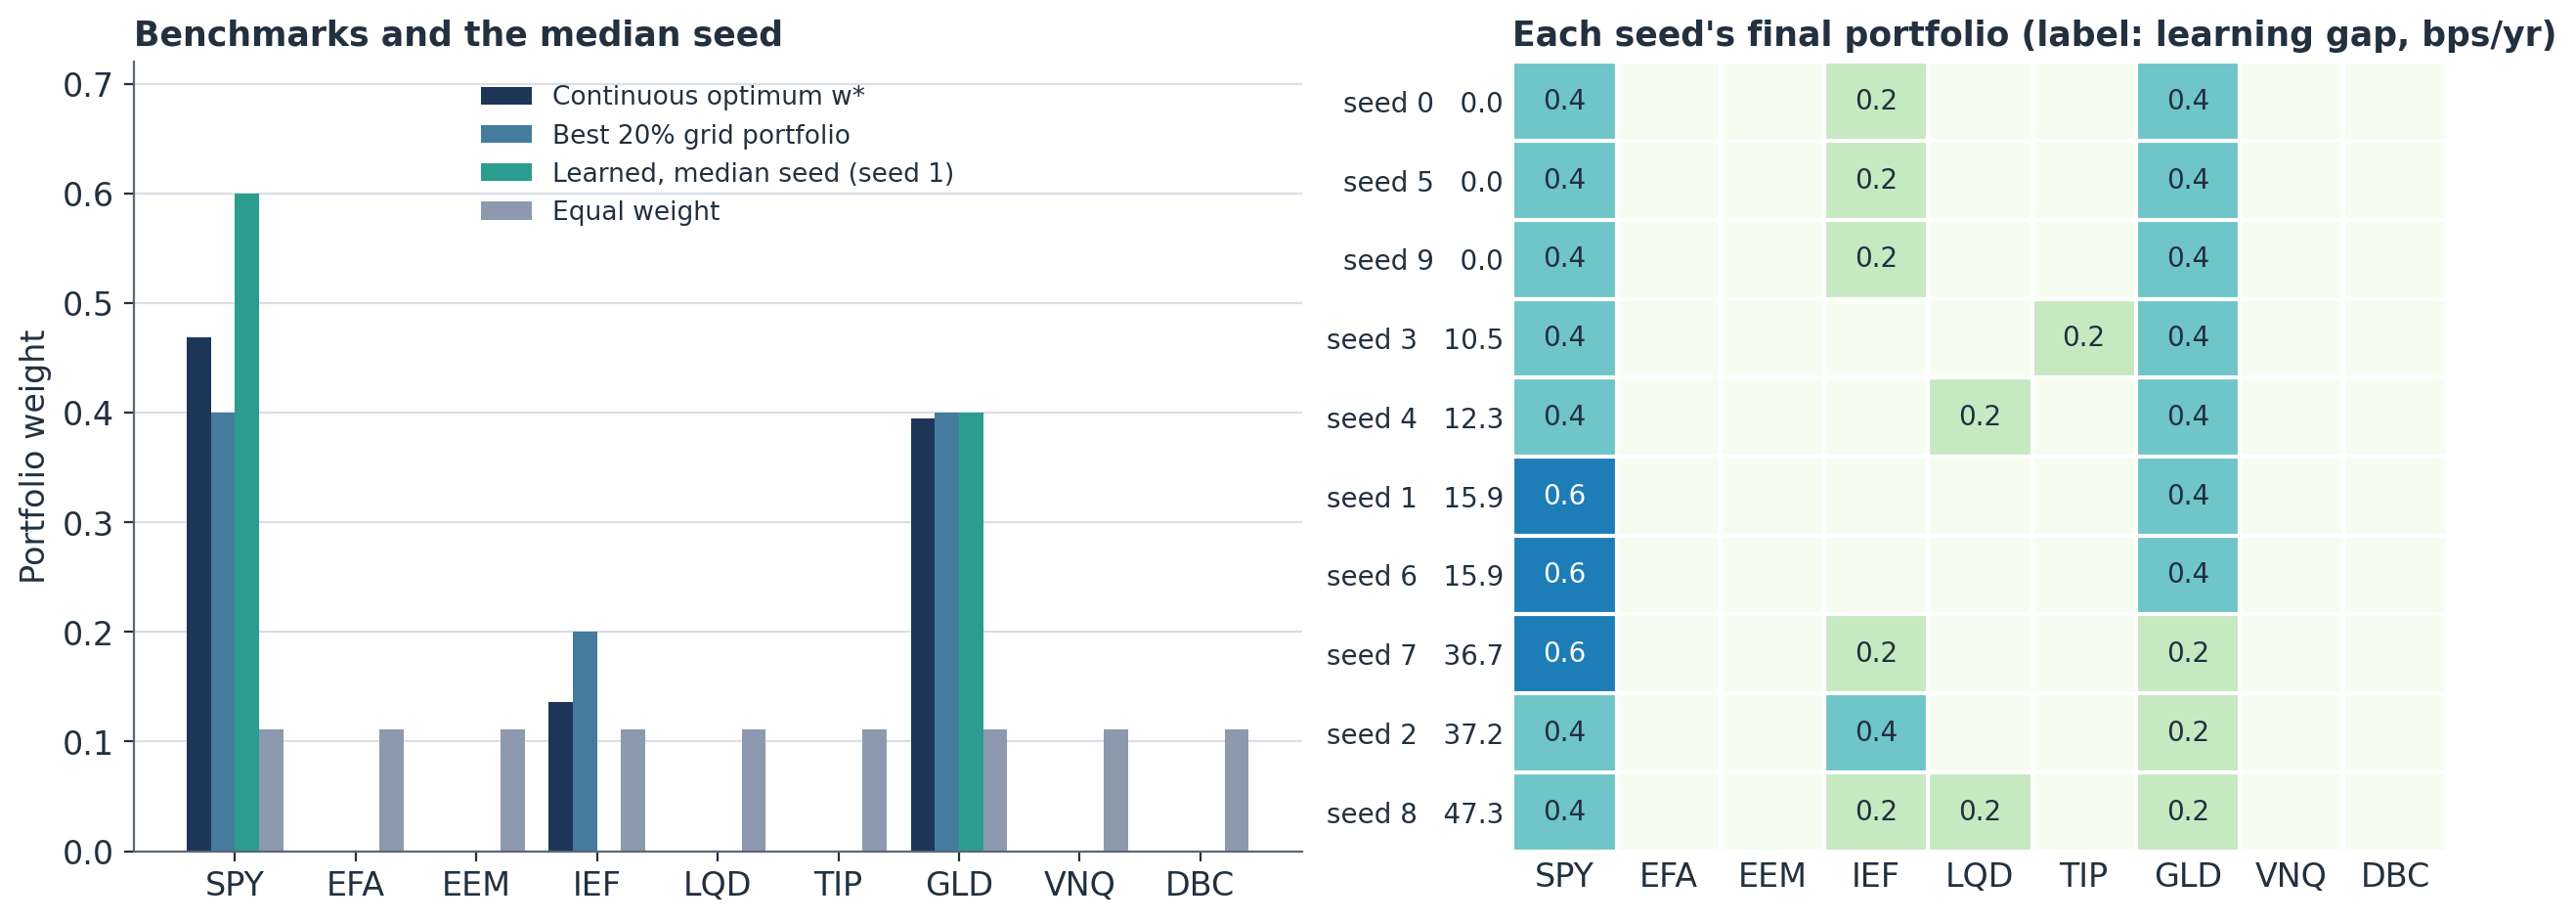
\includegraphics[keepaspectratio,alt={Figure 1. Portfolio weights at γ = 5 on the 20\% grid. Left: the continuous optimum, the best grid portfolio, the median seed by learning gap and equal weight. Right: each seed's final portfolio, ordered by its learning gap in bps/yr.}]{figures/fig_weights.png}}
\caption{\textbf{Figure 1.} Portfolio weights at γ = 5 on the 20\% grid.
Left: the continuous optimum, the best grid portfolio, the median seed
by learning gap and equal weight. Right: each seed's final portfolio,
ordered by its learning gap in bps/yr.}
\end{figure}

\subsubsection{5.4 Economic performance and
gaps}\label{economic-performance-and-gaps}

\begin{table}[htbp]
\centering\small
\caption{\textbf{Table 5.} Performance at γ = 5 on the 20\% grid, from
the exact moments. The column-medians row takes each column's median
across the ten seeds separately, so it matches no single
seed.}
\begin{tabular}{@{}
  >{\raggedright\arraybackslash}p{(\linewidth - 8\tabcolsep) * \real{0.3864}}
  >{\raggedleft\arraybackslash}p{(\linewidth - 8\tabcolsep) * \real{0.1250}}
  >{\raggedleft\arraybackslash}p{(\linewidth - 8\tabcolsep) * \real{0.1250}}
  >{\raggedleft\arraybackslash}p{(\linewidth - 8\tabcolsep) * \real{0.1250}}
  >{\raggedleft\arraybackslash}p{(\linewidth - 8\tabcolsep) * \real{0.2386}}@{}}
\toprule\noalign{}
\begin{minipage}[b]{\linewidth}\raggedright
Portfolio
\end{minipage} & \begin{minipage}[b]{\linewidth}\raggedleft
Return
\end{minipage} & \begin{minipage}[b]{\linewidth}\raggedleft
Volatility
\end{minipage} & \begin{minipage}[b]{\linewidth}\raggedleft
\(U\), bps/yr
\end{minipage} & \begin{minipage}[b]{\linewidth}\raggedleft
Loss vs.~\(w^*\), bps/yr
\end{minipage} \\
\midrule\noalign{}
Continuous optimum & 8.86\% & 11.92\% & 530.5 & 0 \\
Best grid portfolio & 8.28\% & 11.01\% & 524.8 & 5.7 \\
Learned, upper-median seed (seed 1; seed 6 identical) & 10.07\% &
14.12\% & 508.9 & 21.6 \\
Learned, column medians (range) & 8.28\% & 11.11\% & 510.7 & 19.8 (5.7
to 53.1) \\
Equal weight & 5.62\% & 11.71\% & 219.6 & 310.9 \\
\bottomrule\noalign{}
\end{tabular}
\end{table}

Gaps use the known μ and Σ. The 10,000 fresh evaluation episodes give
the best grid portfolio's realized value (485.8 bps/yr) a standard error
of 39.4, enough to confirm only large differences such as equal weight's
shortfall (308.8, standard error 21.1).

\begin{table}[htbp]
\centering\small
\caption{\textbf{Table 6.} Gaps across ten seeds, bps/yr. The total gap
is the discretization gap plus the learning gap.}
\begin{tabular}{@{}
  >{\raggedright\arraybackslash}p{(\linewidth - 8\tabcolsep) * \real{0.1579}}
  >{\raggedleft\arraybackslash}p{(\linewidth - 8\tabcolsep) * \real{0.2105}}
  >{\raggedleft\arraybackslash}p{(\linewidth - 8\tabcolsep) * \real{0.2105}}
  >{\raggedleft\arraybackslash}p{(\linewidth - 8\tabcolsep) * \real{0.2105}}
  >{\raggedleft\arraybackslash}p{(\linewidth - 8\tabcolsep) * \real{0.2105}}@{}}
\toprule\noalign{}
\begin{minipage}[b]{\linewidth}\raggedright
Experiment
\end{minipage} & \begin{minipage}[b]{\linewidth}\raggedleft
Discretization gap
\end{minipage} & \begin{minipage}[b]{\linewidth}\raggedleft
Learning gap, mean / median (range)
\end{minipage} & \begin{minipage}[b]{\linewidth}\raggedleft
Total gap, mean / median
\end{minipage} & \begin{minipage}[b]{\linewidth}\raggedleft
Exactly best grid portfolio
\end{minipage} \\
\midrule\noalign{}
γ = 5, 20\% grid & 5.74 & 17.6 / 14.1 (0 to 47.3) & 23.3 / 19.8 & 3 of
10 \\
γ = 5, 25\% grid & 11.74 & 5.1 / 2.5 (0 to 30.7) & 16.9 / 14.3 & 5 of
10 \\
γ = 3, 20\% grid & 2.47 & 30.6 / 10.0 (0 to 81.1) & 33.0 / 12.5 & 5 of
10 \\
γ = 8, 20\% grid & 6.13 & 13.0 / 5.7 (0 to 53.1) & 19.2 / 11.9 & 5 of
10 \\
\bottomrule\noalign{}
\end{tabular}
\end{table}

The median learned portfolio keeps 96\% of the available
certainty-equivalent return (510.7 of 530.5 bps/yr) and closes 94\% of
the distance from equal weight to the optimum. On the 20\% grid the
learning gap exceeds the discretization gap at every γ in the mean, and
at γ = 5 and γ = 3 in the median. The distribution is skewed (Figure
A5): three to five seeds per experiment have no learning gap, and the
worst is 47.3 bps/yr behind at γ = 5 and 81.1 at γ = 3.

\subsubsection{5.5 Learning curve, regret and action-space
resolution}\label{learning-curve-regret-and-action-space-resolution}

\begin{figure}
\centering
\pandocbounded{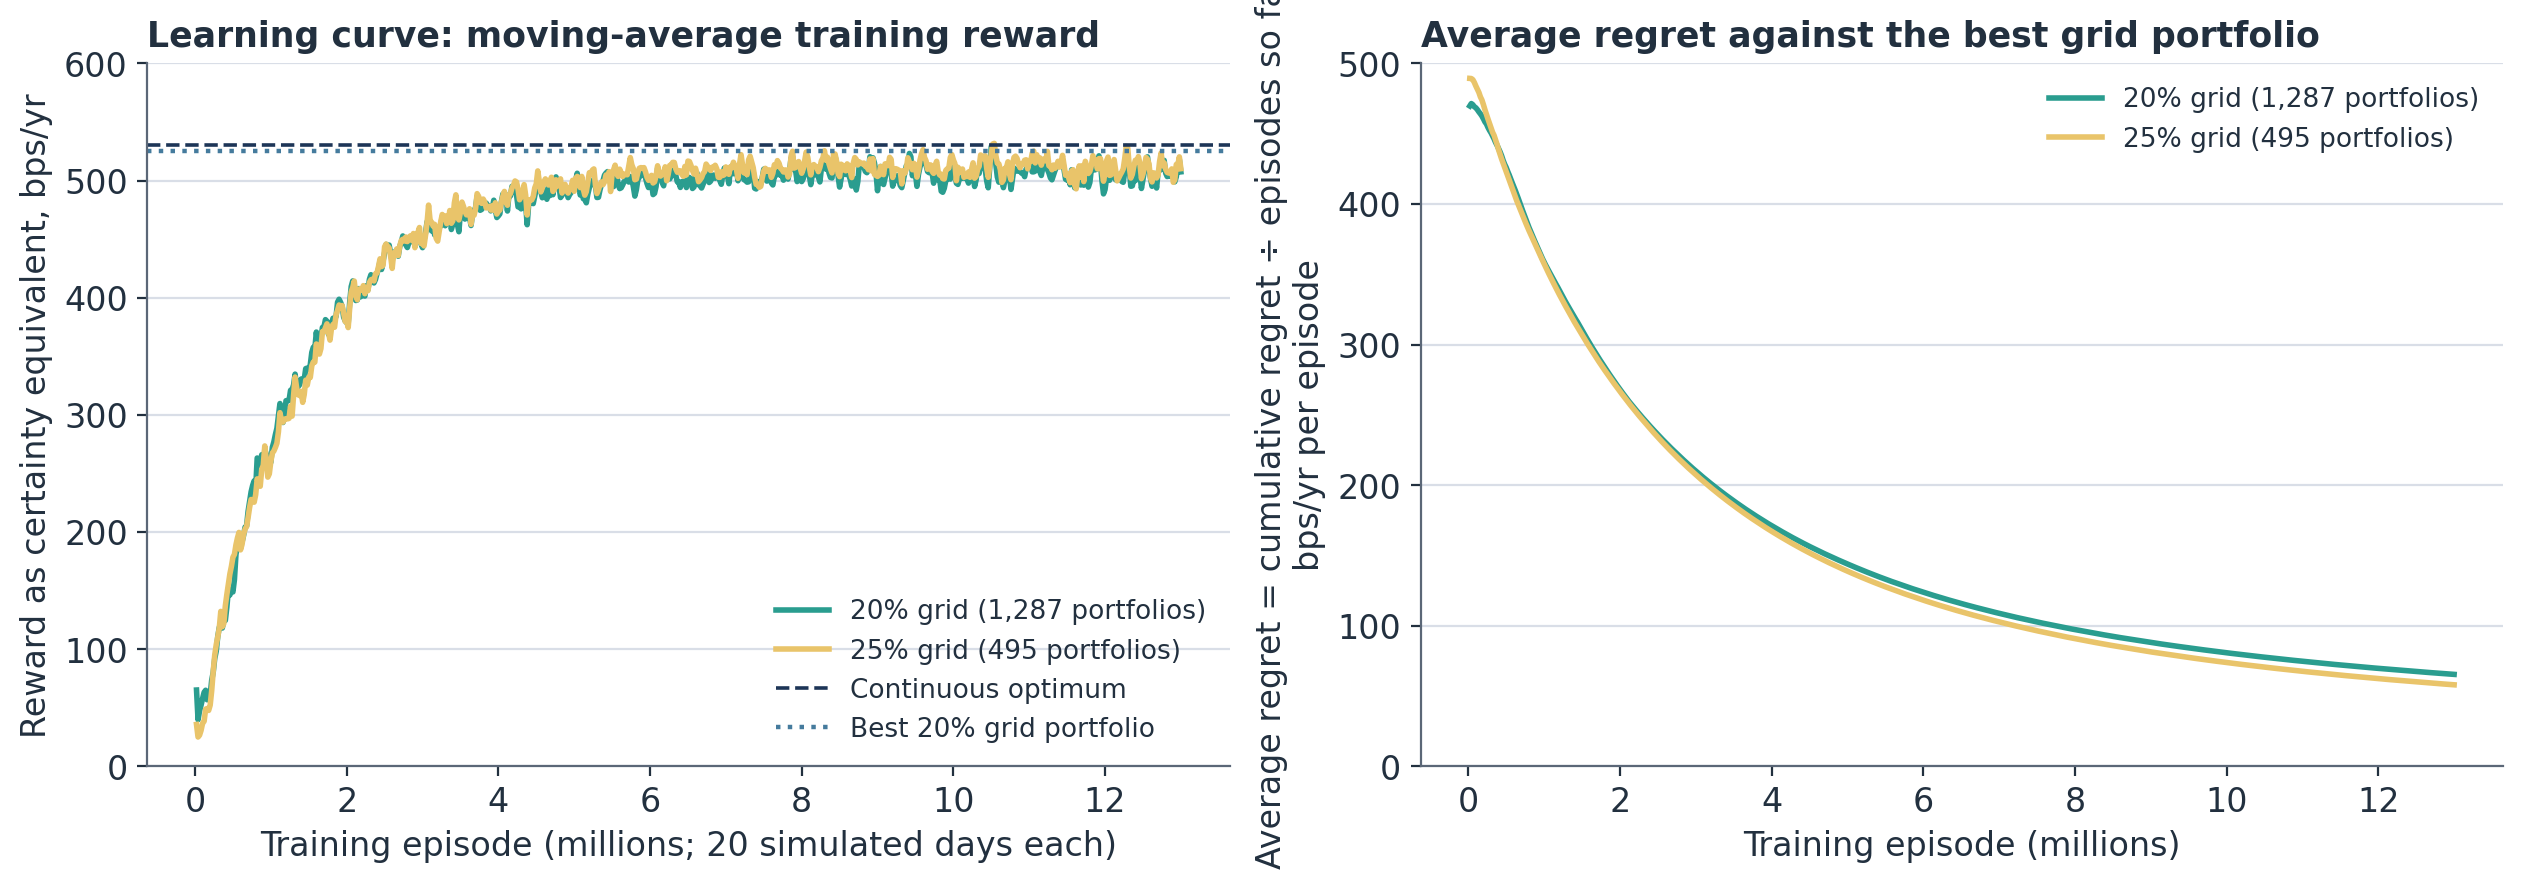
\includegraphics[keepaspectratio,alt={Figure 2. Left: moving-average training reward, median across seeds, as a certainty equivalent; it includes exploratory episodes. Right: average regret, the cumulative regret against each grid's best portfolio divided by the number of episodes so far.}]{figures/fig_learning_curve.png}}
\caption{\textbf{Figure 2.} Left: moving-average training reward, median
across seeds, as a certainty equivalent; it includes exploratory
episodes. Right: average regret, the cumulative regret against each
grid's best portfolio divided by the number of episodes so far.}
\end{figure}

Training reward rises as exploration decays and levels off just below
the best grid portfolio's value from about the halfway episode (Figure
2). Averaged over the run, median regret is 65.5 bps/yr per episode on
the 20\% grid and 58.1 on the 25\% grid. Nearly all of it is the price
of exploration, since the final portfolios' median shortfalls are 14.1
and 2.5 (Table 6).

\begin{figure}
\centering
\pandocbounded{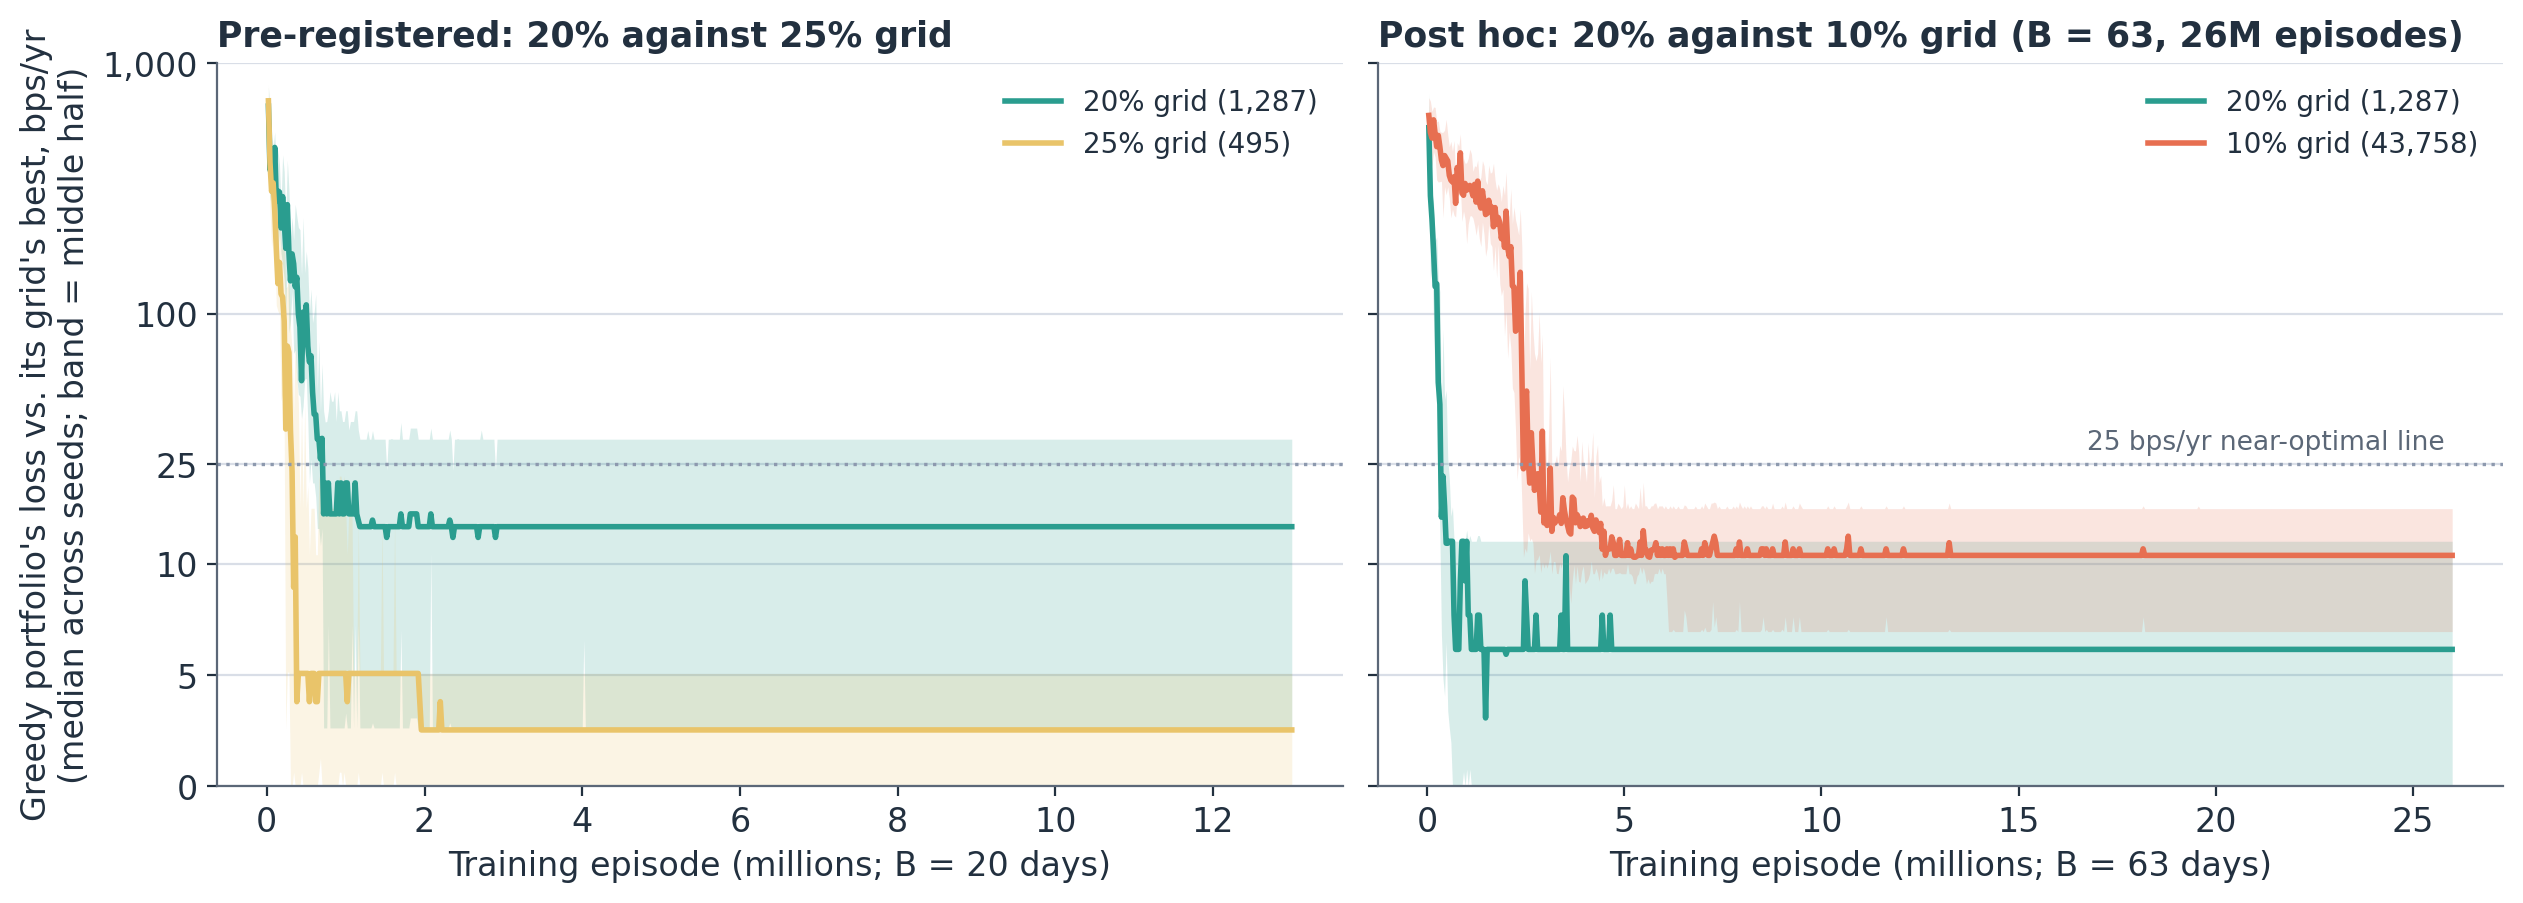
\includegraphics[keepaspectratio,alt={Figure 3. Loss of the greedy portfolio against its own grid's best portfolio during training (median across seeds; the band covers the middle half of seeds; the vertical scale is linear below 10 and logarithmic above). Left: the pre-registered 20\% and 25\% grids. Right: the post hoc 20\% and 10\% grids under longer episodes and a doubled budget (Section 6.1).}]{figures/fig_convergence_resolution.png}}
\caption{\textbf{Figure 3.} Loss of the greedy portfolio against its own
grid's best portfolio during training (median across seeds; the band
covers the middle half of seeds; the vertical scale is linear below 10
and logarithmic above). Left: the pre-registered 20\% and 25\% grids.
Right: the post hoc 20\% and 10\% grids under longer episodes and a
doubled budget (Section 6.1).}
\end{figure}

The 25\% grid, with 495 portfolios, doubles the discretization gap
(11.74 against 5.74 bps/yr) and cuts the median learning gap from 14.1
to 2.5. It meets the primary rule on all ten seeds (median 101.2 million
days, against nine seeds at 185.1 million) and stays within 25 bps/yr
for good sooner (9.6 against 25.8 million days). Its median total gap is
lower (14.3 against 19.8), so at this budget the coarser grid is the
better choice at γ = 5.

\subsubsection{5.6 What prevented exact
recovery}\label{what-prevented-exact-recovery}

The agent must rank portfolios whose expected rewards are nearly equal
from very noisy samples. At γ = 5 the second-best grid portfolio (TIP in
place of IEF) is 10.5 bps/yr behind the best, and one episode's reward
has a standard deviation near 3,900 bps/yr. Separating the two at two
standard errors takes about 1.1 million evaluations of each; exploration
gives each portfolio about 1,097. In the seven seeds that missed the
best portfolio it was tried 1,118 to 4,282 times (Figure A8). Once ε is
small the agent revisits only its current favorite, so a portfolio whose
early sample mean was unlucky is rarely tried again. A post hoc
diagnostic fits this account: across the whole grid the learned Q-values
order portfolios much as true utility does (median rank correlation
0.821), but only about a third of the ten truly best portfolios appear
in the agent's own top ten (median 3.5 of 10).

\subsection{6. Robustness, research challenges, and
limitations}\label{robustness-research-challenges-and-limitations}

Section 6.1 changes the action-space design and Section 6.2 the economic
and statistical assumptions; apart from risk aversion and the 25\% grid,
every run here is post hoc. Sections 6.3 to 6.5 cover the two bonus
extensions and the six research challenges.

\subsubsection{6.1 Action-space design: the 10\% grid (post
hoc)}\label{action-space-design-the-10-grid-post-hoc}

The 10\% grid has 43,758 portfolios, 34 times the baseline. It was run
with \(B\) = 63, 26 million episodes and ε = 3\% at halfway, so its
comparison is the 20\% grid under the same settings (\texttt{all-three},
Section 6.2). Expected directions were registered before training.

\begin{table}[htbp]
\centering\small
\caption{\textbf{Table 7.} The 20\% and 10\% grids under identical
settings (B = 63, 26 million episodes, ε = 3\% at halfway), ten seeds
each, bps/yr. The paired change is the 10\% grid's total gap minus the
20\% grid's, seed by seed.}
\begin{tabular}{@{}
  >{\raggedright\arraybackslash}p{(\linewidth - 10\tabcolsep) * \real{0.1304}}
  >{\raggedleft\arraybackslash}p{(\linewidth - 10\tabcolsep) * \real{0.1739}}
  >{\raggedleft\arraybackslash}p{(\linewidth - 10\tabcolsep) * \real{0.1739}}
  >{\raggedleft\arraybackslash}p{(\linewidth - 10\tabcolsep) * \real{0.1739}}
  >{\raggedleft\arraybackslash}p{(\linewidth - 10\tabcolsep) * \real{0.1739}}
  >{\raggedleft\arraybackslash}p{(\linewidth - 10\tabcolsep) * \real{0.1739}}@{}}
\toprule\noalign{}
\begin{minipage}[b]{\linewidth}\raggedright
γ
\end{minipage} & \begin{minipage}[b]{\linewidth}\raggedleft
Discretization gap, 20\% → 10\%
\end{minipage} & \begin{minipage}[b]{\linewidth}\raggedleft
Mean learning gap, 20\% → 10\%
\end{minipage} & \begin{minipage}[b]{\linewidth}\raggedleft
Exactly best, 20\% → 10\%
\end{minipage} & \begin{minipage}[b]{\linewidth}\raggedleft
Paired change in total gap (SE)
\end{minipage} & \begin{minipage}[b]{\linewidth}\raggedleft
Primary rule met, 20\% → 10\%
\end{minipage} \\
\midrule\noalign{}
5 & 5.7 → 1.3 & 7.9 → 11.7 & 5 → 0 of 10 & −0.6 (3.7) & 10 → 0 of 10 \\
3 & 2.5 → 2.5 & 4.0 → 22.0 & 8 → 4 of 10 & +18.0 (7.5) & 10 → 0 of 10 \\
8 & 6.1 → 6.1 & 1.1 → 5.8 & 9 → 1 of 10 & +4.6 (1.6) & 10 → 0 of 10 \\
\bottomrule\noalign{}
\end{tabular}
\end{table}

At γ = 5 the finer grid removes 4.4 bps/yr of discretization error and
none of it reaches the learned portfolio (paired change in the total gap
−0.6, standard error 3.7). At γ = 3 and γ = 8 the best portfolio is the
same on both grids, so the finer grid only adds learning error (+18.0
and +4.6). No seed of the thirty meets the primary rule. Exploration
gives each portfolio about 85 visits, and at γ = 5 the best portfolio
was tried a median of 116 times per seed while each final portfolio was
tried 19 to 22 million times. The weights reported for these seeds are
therefore final greedy portfolios that never met the convergence rule.
The economic rule still holds for 10, 5 and 10 seeds at γ = 5, 3 and 8,
so the agent reaches the right neighborhood and keeps moving within it
(Figures 3 and A9). The registered directions held for the learning gap,
the discretization gap and convergence. The expectation that almost no
seed would find the exact best portfolio failed at γ = 3, where four did
and the runner-up is only 0.04 bps/yr behind. A larger budget on this
grid was not tested.

\subsubsection{6.2 Economic and statistical
assumptions}\label{economic-and-statistical-assumptions}

\textbf{Risk aversion (pre-registered).} Tables 2 and 6 give the results
for γ = 3 and γ = 8, and the learned portfolios move toward Treasuries
with the optimum (Section 5.3). The median learning gap is 10.0 bps/yr
at γ = 3 and 5.7 at γ = 8, against 14.1 at γ = 5, with five exact seeds
at each. The mean is largest at γ = 3 (30.6) because four seeds end more
than 55 bps/yr behind.

\textbf{Episode length, training budget and exploration (post hoc).}
Four tabular variants were registered before they ran. Each changes one
baseline setting, and the fourth changes all three (Table 8, Figure
A10).

\begin{table}[htbp]
\centering\small
\caption{\textbf{Table 8.} Mean learning gap on the 20\% grid, bps/yr,
ten seeds; Δ is the change from the baseline, with its standard error in
parentheses. The runs share starting seeds but not draws, so the
standard errors are approximate.}
\begin{tabular}{@{}
  >{\raggedright\arraybackslash}p{(\linewidth - 14\tabcolsep) * \real{0.1287}}
  >{\raggedright\arraybackslash}p{(\linewidth - 14\tabcolsep) * \real{0.2475}}
  >{\raggedleft\arraybackslash}p{(\linewidth - 14\tabcolsep) * \real{0.0792}}
  >{\raggedleft\arraybackslash}p{(\linewidth - 14\tabcolsep) * \real{0.1287}}
  >{\raggedleft\arraybackslash}p{(\linewidth - 14\tabcolsep) * \real{0.0792}}
  >{\raggedleft\arraybackslash}p{(\linewidth - 14\tabcolsep) * \real{0.1287}}
  >{\raggedleft\arraybackslash}p{(\linewidth - 14\tabcolsep) * \real{0.0792}}
  >{\raggedleft\arraybackslash}p{(\linewidth - 14\tabcolsep) * \real{0.1287}}@{}}
\toprule\noalign{}
\begin{minipage}[b]{\linewidth}\raggedright
Run
\end{minipage} & \begin{minipage}[b]{\linewidth}\raggedright
Change from baseline
\end{minipage} & \begin{minipage}[b]{\linewidth}\raggedleft
γ = 5 gap
\end{minipage} & \begin{minipage}[b]{\linewidth}\raggedleft
γ = 5 Δ (SE)
\end{minipage} & \begin{minipage}[b]{\linewidth}\raggedleft
γ = 3 gap
\end{minipage} & \begin{minipage}[b]{\linewidth}\raggedleft
γ = 3 Δ (SE)
\end{minipage} & \begin{minipage}[b]{\linewidth}\raggedleft
γ = 8 gap
\end{minipage} & \begin{minipage}[b]{\linewidth}\raggedleft
γ = 8 Δ (SE)
\end{minipage} \\
\midrule\noalign{}
Baseline & & 17.6 & & 30.6 & & 13.0 & \\
\texttt{b63} & \(B\) = 63 days & 5.1 & −12.5 (6.2) & 10.0 & −20.6 (10.4)
& 9.1 & −3.9 (6.6) \\
\texttt{n26m} & 26 million episodes & 8.3 & −9.3 (5.3) & 16.2 & −14.3
(14.7) & 5.0 & −8.0 (7.2) \\
\texttt{eps-decay} & ε = 3\% at halfway & 16.1 & −1.5 (7.2) & 4.0 &
−26.6 (11.1) & 11.6 & −1.4 (9.2) \\
\texttt{all-three} & All of the above & 7.9 & −9.7 (5.9) & 4.0 & −26.6
(11.7) & 1.1 & −11.9 (5.4) \\
\bottomrule\noalign{}
\end{tabular}
\end{table}

With \(B\) = 63 the median gap at γ = 5 falls from 14.1 to 0.0 and six
seeds are exact against three, but a 63-day episode uses three times the
simulated data. Doubling the episodes lowers the mean gap at every γ,
while the medians move both ways (14.1 to 10.5, 10.0 to 20.0, 5.7 to
0.0), and still gives only about 2,200 random visits per portfolio, far
below the million needed to separate the top two. Slower exploration
decay changes little at γ = 5 and γ = 8 and raises training regret (65.5
to 77.3 bps/yr per episode at γ = 5). All three changes together give
the best tabular results (median gaps of 6.2, 0.0 and 0.0, and all
thirty seeds meet the primary rule) without showing which change
matters. Most single differences are within two standard errors of zero;
the exceptions are \texttt{b63} at γ = 5, \texttt{eps-decay} and
\texttt{all-three} at γ = 3, and \texttt{all-three} at γ = 8.
Alternative calibration windows, shrinkage covariance estimates and
fat-tailed returns were not run.

\subsubsection{6.3 Extension: function approximation (post
hoc)}\label{extension-function-approximation-post-hoc}

A table treats the 1,287 portfolios as unrelated, though portfolios with
similar weights have similar utility. Function approximation replaces it
with \(\hat{Q}(a) = \theta^\top \phi(w_a)\), updated by stochastic
gradient steps on the same rewards. We use quadratic features (45
columns), which match the form of \(U\) and serve as a correctly
specified reference, and additive and pairwise cubic B-splines (909
columns, rank 369 on the 20\% grid), which assume only smoothness.
Shared parameters have no \(1/N(a)\) rule, so these runs use a constant
step size, tuned at γ = 5 on separate seeds by scoring fully trained
agents on simulated evaluation episodes. An investor with one return
history could not validate this way, but no closed-form benchmark
entered the choice. The like-for-like comparison is therefore a
constant-step table (\texttt{tabular-const}, α = 3.2 × 10⁻⁴). All runs
were registered before training.

\begin{table}[htbp]
\centering\small
\caption{\textbf{Table 9.} Mean learning gap, bps/yr, ten seeds. The
10\% grid runs use B = 63 and 26 million episodes.}
\begin{tabular}{@{}llrrr@{}}
\toprule\noalign{}
Grid & Run & γ = 5 & γ = 3 & γ = 8 \\
\midrule\noalign{}
20\% & Table, α = 1/N (baseline) & 17.6 & 30.6 & 13.0 \\
20\% & Table, constant α & 43.5 & 107.2 & 43.3 \\
20\% & Quadratic features & 22.6 & 8.0 & 58.7 \\
20\% & Splines & 15.7 & 45.4 & 54.6 \\
10\% & Table, α = 1/N & 11.7 & 22.0 & 5.8 \\
10\% & Splines, ε = 3\% at halfway & 78.8 & 140.6 & 59.6 \\
10\% & Splines, ε = 10\% at halfway & 81.4 & 155.6 & 60.2 \\
\bottomrule\noalign{}
\end{tabular}
\end{table}

A constant step raises the table's mean gap at every γ (+25.9, +76.6 and
+30.2 bps/yr; standard errors 11.5, 24.6 and 8.0). All ten constant-step
seeds at γ = 5 met the primary rule without holding the best portfolio,
so under a constant step that rule measures stability more than
accuracy. On the 20\% grid, splines beat the constant-step table at γ =
5 and γ = 3 (−27.8 and −61.8; standard errors 11.9 and 24.2) and lose at
γ = 8 (+11.4, standard error 5.1). Against the \(1/N\) baseline they are
level at γ = 5 (−1.8, standard error 9.5) and 41.6 bps/yr worse at γ = 8
(standard error 6.0). One hypothesis, which we have not tested, is that
at γ = 8 most directions of the parameter vector have not finished
learning within the budget.

\begin{figure}
\centering
\pandocbounded{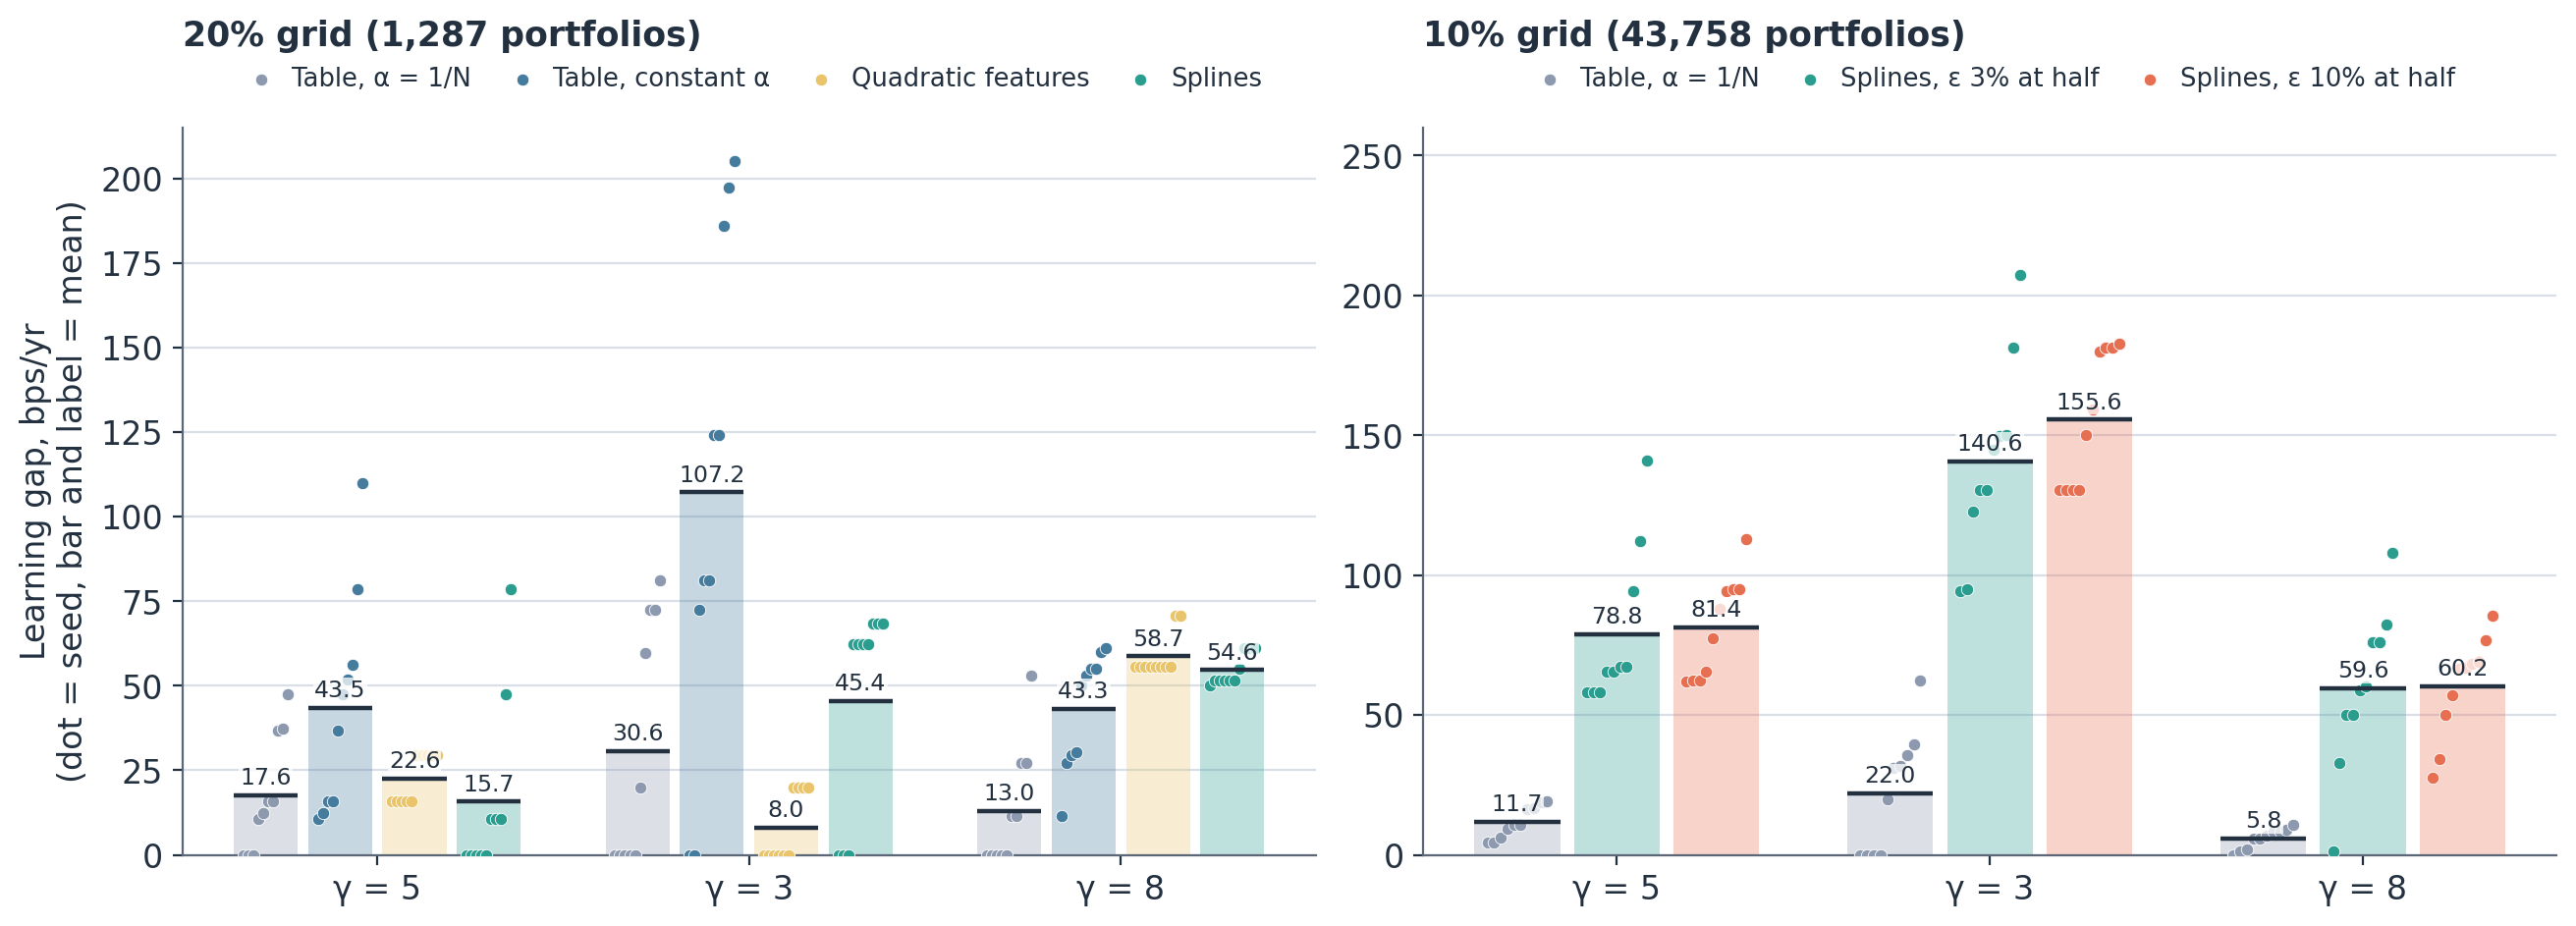
\includegraphics[keepaspectratio,alt={Figure 4. Learning gap for every seed (dots) and its mean (bar and label). Left: the 20\% grid. Right: the 10\% grid, where function approximation was expected to help most.}]{figures/fig_fa.png}}
\caption{\textbf{Figure 4.} Learning gap for every seed (dots) and its
mean (bar and label). Left: the 20\% grid. Right: the 10\% grid, where
function approximation was expected to help most.}
\end{figure}

On the 10\% grid, the setting that motivated the extension, splines lose
to the \(1/N\) table: mean gaps of 78.8, 140.6 and 59.6 bps/yr against
11.7, 22.0 and 5.8 (paired differences +67.1, +118.6 and +53.8; standard
errors 9.1, 12.2 and 9.8), worse on 29 of 30 seeds. The comparison is
confounded. No constant-step table ran on this grid, the constant step
alone costs the table 26 to 77 bps/yr on the 20\% grid, and the spline
step (2.778 × 10⁻⁵) was matched to the noise level without re-tuning.
More exploration (ε = 10\% at halfway) does not help (+2.6, +15.0 and
+0.6, each within about one standard error), and no seed of the sixty
meets the primary rule. At γ = 5 splines rank the whole grid far better
than the table (median Spearman correlation 0.976 against 0.543), yet at
the median none of the true top ten is in their own top ten (Table A1,
Figure A11). Every seed under-weights SPY, holding 20\% to 40\% where
the best portfolio holds 50\%, 60\% and 40\% at γ = 5, 3 and 8. We
report the 10\% grid outcome as a negative result for this
configuration.

\subsubsection{6.4 Extension: transaction costs and rebalancing (post
hoc)}\label{extension-transaction-costs-and-rebalancing-post-hoc}

\textbf{A first design that failed.} The first design kept the nine
assets and the 20\% grid, made the state the previous portfolio and
charged a quadratic cost for moving. That gives 1.66 million (holding,
target) pairs and, with holdings that never drift, no reason to
rebalance. At zero cost the median learned policy scored 56.6 bps/yr
against the oracle's 524.8, about the average over all 1,287 grid
portfolios (56.7), so we redesigned the problem (Table A2, Figure A13).

\textbf{The redesign.} The universe is the three ETFs in the nine-asset
optimum (SPY, IEF, GLD), with γ = 5. Time runs in blocks of 63 trading
days. Share counts are fixed within a block, so the weights drift with
returns and the drifted weights are the next block's state (Figure A12).
At the start of each block the agent holds or trades to one of 1,326
targets on a 2\% grid, paying a fraction of wealth

\[c(s, x) = \kappa \lVert x - s \rVert_1 + \frac{\lambda}{2} \lVert x - s \rVert_2^2\]

to move from holdings \(s\) to target \(x\): a proportional term for the
bid-ask spread and a quadratic term for price impact, in the spirit of
Gârleanu and Pedersen (2013). The block reward is the Section 4 reward
on the drifting portfolio minus the cost spread over 63 days. The agent
maximizes the discounted sum of block rewards with a discount factor of
0.95 per block (about 0.81 per year), which now matters because a trade
sets the next block's holdings. κ and λ come from the ETFs' quoted
spreads and volume under a square-root impact model at three fund sizes:
\$100 million (κ = 1.63 bp, λ = 4.4 × 10⁻³), \$1 billion (3.90 bp, 1.43
× 10⁻²) and \$10 billion (11.04 bp, 4.57 × 10⁻²), plus a zero-cost
control.

\textbf{Benchmarks.} The oracle solves the same problem by value
iteration on a 1\% lattice, knowing μ, Σ, κ and λ. Three reference
policies share its simulated paths: always rebalance to the best no-cost
target (46/14/40), trade to that target once and then hold, and a myopic
policy that optimizes one block at a time. Every policy is scored by
expected discounted utility over 4,000 shared starting points and
90-block paths, in bps/yr. The oracle beats always rebalancing by only
0.04, 0.42, 1.78 and 7.79 bps/yr at zero cost, \$100 million, \$1
billion and \$10 billion (standard errors 0.04, 0.22, 0.36 and 0.64), in
line with its in-model lead (0.01, 0.21, 1.32 and 6.94), so the gain
available from timing trades is small.

\textbf{Agent.} The agent uses a linear Q-function with 87 spline
features of the post-trade weights and two cost features, the L1 and
squared L2 size of the trade, whose coefficients it learns from net
rewards. It never sees μ, Σ, κ, λ or the oracle. Each seed trains for 4
million blocks; the step size (3 × 10⁻⁴) was tuned on a separate seed at
\$1 billion, and the reported policy averages the parameters over the
last 10\% of training. Twelve expectations were registered before any
final run (Table A3).

\begin{table}[htbp]
\centering\small
\caption{\textbf{Table 10.} Value of each policy, bps/yr of expected
discounted utility. The agent's value is the mean of ten
seeds.}
\begin{tabular}{@{}lrrrr@{}}
\toprule\noalign{}
Policy & Zero cost & \$100M & \$1B & \$10B \\
\midrule\noalign{}
Oracle & 531.52 & 530.16 & 528.09 & 523.22 \\
Myopic & 531.52 & 530.18 & 527.96 & 520.95 \\
Always rebalance & 531.48 & 529.75 & 526.31 & 515.44 \\
Agent (mean of 10 seeds) & 518.37 & 517.07 & 518.11 & 520.45 \\
Trade once, then hold & 508.49 & 507.22 & 504.56 & 496.11 \\
\bottomrule\noalign{}
\end{tabular}
\end{table}

\textbf{Results.} The agent trails the oracle at every level and on all
forty seeds, and the gap narrows as costs rise: 13.1 bps/yr at zero cost
and at \$100 million, 10.0 at \$1 billion and 2.8 at \$10 billion. Seeds
differ by more than the evaluation noise (standard deviation across
seeds 4.3 to 5.5 bps/yr below \$10 billion, against a path standard
error near 1). Scoring a third policy, always rebalancing to the agent's
own favorite target, splits the agent's gap to always rebalancing into
target choice and trade timing (Table 11, Figure 5).

\begin{table}[htbp]
\centering\small
\caption{\textbf{Table 11.} The agent against the references, mean of
ten seeds. Target choice compares always rebalancing to the agent's own
favorite target with always rebalancing to the best target; trade timing
compares the agent with always rebalancing to its own target. The two
sum to agent − always rebalance, up to rounding.}
\begin{tabular}{@{}
  >{\raggedright\arraybackslash}p{(\linewidth - 8\tabcolsep) * \real{0.4894}}
  >{\raggedleft\arraybackslash}p{(\linewidth - 8\tabcolsep) * \real{0.1277}}
  >{\raggedleft\arraybackslash}p{(\linewidth - 8\tabcolsep) * \real{0.1277}}
  >{\raggedleft\arraybackslash}p{(\linewidth - 8\tabcolsep) * \real{0.1277}}
  >{\raggedleft\arraybackslash}p{(\linewidth - 8\tabcolsep) * \real{0.1277}}@{}}
\toprule\noalign{}
\begin{minipage}[b]{\linewidth}\raggedright
\end{minipage} & \begin{minipage}[b]{\linewidth}\raggedleft
Zero cost
\end{minipage} & \begin{minipage}[b]{\linewidth}\raggedleft
\$100M
\end{minipage} & \begin{minipage}[b]{\linewidth}\raggedleft
\$1B
\end{minipage} & \begin{minipage}[b]{\linewidth}\raggedleft
\$10B
\end{minipage} \\
\midrule\noalign{}
\textbf{A. Value gap, bps/yr} & & & & \\
Agent − oracle (SD across seeds) & −13.14 (4.58) & −13.09 (5.52) & −9.99
(4.32) & −2.77 (1.70) \\
Agent − always rebalance & −13.11 & −12.67 & −8.21 & +5.01 \\
\quad from target choice & −13.11 & −12.75 & −9.04 & −1.14 \\
\quad from trade timing & 0.00 & 0.08 & 0.83 & 6.16 \\
\textbf{B. Trading and convergence, agent (oracle)} & & & & \\
Share of blocks with no trade & 0.35 (0.15) & 0.25 (0.28) & 0.18 (0.32)
& 0.17 (0.45) \\
Turnover per block & 2.06\% (2.88\%) & 2.28\% (2.20\%) & 2.36\% (2.08\%)
& 2.11\% (1.55\%) \\
Seeds converged, final rule (of 10) & 5 & 7 & 7 & 4 \\
\bottomrule\noalign{}
\end{tabular}
\end{table}

\begin{figure}
\centering
\pandocbounded{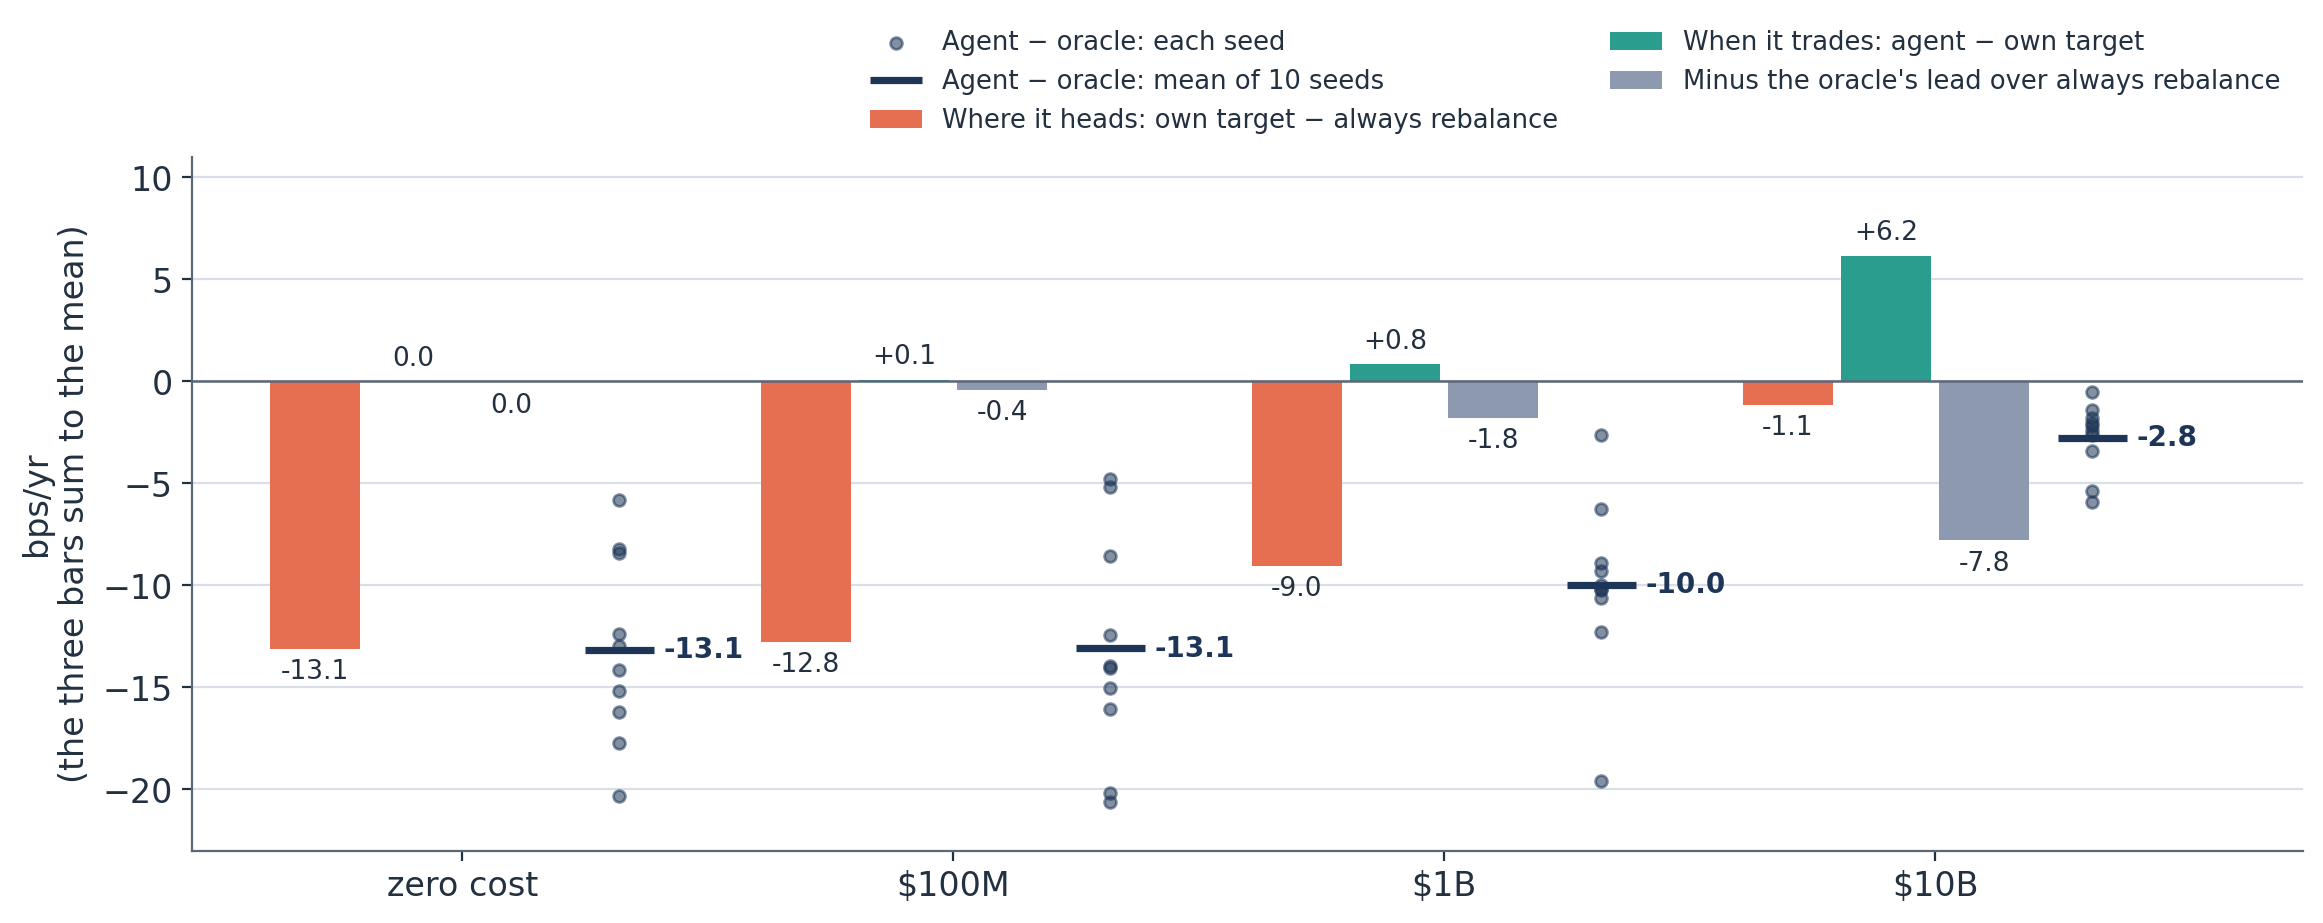
\includegraphics[keepaspectratio,alt={Figure 5. The agent's gap to the oracle by cost level, split into the portfolio it aims for, its decisions about when to trade, and the oracle's lead over always rebalancing. The three bars sum to the mean gap. Dots are the ten seeds.}]{figures/fig_tc_split.png}}
\caption{\textbf{Figure 5.} The agent's gap to the oracle by cost level,
split into the portfolio it aims for, its decisions about when to trade,
and the oracle's lead over always rebalancing. The three bars sum to the
mean gap. Dots are the ten seeds.}
\end{figure}

At the three lower levels almost all of the gap is target choice. The
favorite target loses 13.1, 12.8 and 9.0 bps/yr against the best target,
and timing adds 0.0, 0.1 and 0.8. Every favorite target there holds 18\%
to 32\% in IEF against 14\% in the best target (Figure A15), and the
agent loses on all ten seeds to always rebalancing, a rule handed the
best target from μ and Σ.

At \$10 billion trade timing is worth +6.2 bps/yr, against the oracle's
7.8 lead over always rebalancing, and the favorite target loses only
1.1. The agent beats always rebalancing on all ten seeds (by 5.0 on
average, 1.9 to 7.3) and is statistically indistinguishable from the
myopic policy, which knows μ, Σ and the costs (−0.5, across-seed
standard error 0.54; ahead on five seeds). It holds in 17\% of blocks
against the oracle's 45\%, and its turnover (2.11\% per block) lies
between the oracle's (1.55\%) and always rebalancing's (2.98\%).

The agent learns the quadratic cost coefficient, within a factor of two
of the truth on 9 of 10 seeds at \$100 million and all ten at \$1
billion and \$10 billion. It does not learn the linear one: below 0.2 of
the truth on all ten seeds at \$10 billion, at or below 0.15 on six at
\$1 billion, and 2.8 to 14.9 times too high on five at \$100 million
(Figure A17). Of the twelve registered expectations, eight were met and
four partly met (Table A3). The largest miss is the first: we predicted
a gap to the oracle of 1 to 8 bps/yr and observed 13.1, 13.1 and 10.0 at
the lower levels, because the three-seed tuning pilot understated the
favorite target's utility loss (2 to 6 bps/yr there, 9.75 at \$1 billion
here).

\textbf{Disclosures.} The forty runs are post hoc. Benchmark information
shaped the design and never reached the agent during training: the
universe is the support of the nine-asset optimum, the cost levels were
chosen with the oracle's results in view, the cost features fix the
cost's functional form, and the convergence rule was revised three times
before it was frozen. The full list is in Appendix C.

\subsubsection{6.5 Research challenges and
limitations}\label{research-challenges-and-limitations}

\textbf{Estimation error.} μ and Σ come from one 5,152-day sample and
are then treated as known. Annualized means have standard errors of 1.4
to 6.4 percentage points (Table 1). SPY's, 4.27, exceeds the difference
in means for 17 of the 36 asset pairs, so the optimum's concentration in
SPY and GLD rests on estimates the data cannot separate from several
alternatives. Our results are conditional on the calibrated moments and
say nothing about the optimum's out-of-sample performance. We ran
neither another calibration window nor a shrinkage estimate of Σ.

\textbf{Conditioning and numerical stability.} Σ has condition number
268 (smallest eigenvalue \(3.10 \times 10^{-6}\)), well enough behaved
for a stable Cholesky factor in the simulator. The budget-only closed
form, which inverts Σ, is the exposed object. It answers the three
near-collinear equity funds with offsetting bets (182\% SPY against
−88\% EFA at γ = 5) and does the same with IEF and TIP (+27\% and
−27\%). The long-only optimum cannot short, holds three ETFs and avoids
this sensitivity.

\textbf{The curse of dimensionality.} The action set grows from 495 to
3,108,105 portfolios as the step falls from 25\% to 5\%. Random visits
per portfolio fall from about 1,097 on the 20\% grid to 85 on the 10\%
grid even with twice the episodes, and no seed converges there. Spline
function approximation with a constant step did worse than the table on
that grid (Section 6.3), and the first transaction-cost design, with
1.66 million state-action pairs, learned nothing (Section 6.4). In each
case the limit is reward noise relative to the utility differences that
matter, together with the number of alternatives.

\textbf{Discretization error and benchmark leakage.} Discretization and
learning gaps are reported separately throughout. The action set uses
only the asset count and the step, tests stop agent code from importing
benchmark code, and each human design choice that used benchmark
information is disclosed (Sections 4 and 6.4).

\textbf{Consistency between reward and objective.} With the \(B-1\)
divisor, \(E[R \mid w] = U(w)\) exactly, which unit tests verify by
simulation. In the transaction-cost extension the reward is net of cost
on drifting weights, so its expectation is not exactly \(U\) of the
starting weights; the oracle maximizes the same discounted objective.

\textbf{The limits of a stationary simulated environment.} Returns are
independent Gaussian draws with fixed moments, with no regimes, no
predictability and no fat tails, although excess kurtosis in the data
reaches 58.9 (LQD). The baseline uses 260 million simulated days per
seed, about a million years of data, to choose among portfolios that an
investor with twenty years of data could not tell apart. Sample
averaging works here because the moments never change; with drifting
moments the \(1/N\) rule would stop adapting. The learning problem is
solvable in principle at a large cost in data, and whether the method
works on historical returns is left open.

\subsection{7. Conclusion}\label{conclusion}

\textbf{What the agent learned.} From rewards alone, with no knowledge
of expected returns or covariances, the agent learned to hold U.S.
equities and gold on every seed and a bond fund on most, the composition
of the mean-variance optimum, and it moved toward bonds as risk aversion
rose.

\textbf{How close it came.} At γ = 5 on the 20\% grid the median seed is
14.1 bps/yr from the best attainable portfolio and 19.8 from the
continuous optimum, out of 530.5 available; equal weighting loses 310.9.
Three seeds of ten recover the best grid portfolio at γ = 5 and five at
γ = 3 and γ = 8. At γ = 5 nine of ten meet the convergence rule set in
advance.

\textbf{What prevented exact recovery.} The top grid portfolios are
about 10 bps/yr apart while one episode's reward has a standard
deviation near 3,900. Ranking them reliably takes about a million
evaluations of each, and exploration supplies about a thousand. The
agent finds the right region and stops on one of several near-equivalent
portfolios inside it.

\textbf{The trade-off in action-space design.} A finer grid removes
discretization error and adds learning error. Under the same longer
settings the two roughly cancel between the 20\% and 10\% grids at γ =
5, and the 10\% grid is worse at γ = 3 and γ = 8. At the baseline budget
the 25\% grid has a smaller median total gap than the 20\% grid (14.3
against 19.8).

\textbf{The extensions.} Both are post hoc and both include a negative
result. Spline function approximation ranks a large action set well and
picks badly at the top; on the 10\% grid it loses to the \(1/N\) table,
in a comparison that also changes the step-size rule. With transaction
costs, the first design learned nothing. The redesigned agent, which
never sees μ, Σ or the costs, closes in on the full-information oracle
as costs rise (13.1 bps/yr behind at zero cost, 2.8 at \$10 billion). At
\$10 billion its trade timing is worth 6.2 bps/yr and it is
statistically indistinguishable from the myopic policy, but most of the
narrowing comes from a better target at that level, which we have not
explained.

\textbf{Limits.} These results hold in a stationary Gaussian world whose
moments are taken as true, with a data budget no investor has. The
pre-registered experiments carry the headline; the post hoc runs support
it.

\subsection{References}\label{references}

Barsky, R. B., Juster, F. T., Kimball, M. S., and Shapiro, M. D. (1997).
Preference parameters and behavioral heterogeneity: An experimental
approach in the Health and Retirement Study. \emph{Quarterly Journal of
Economics}, 112(2), 537--579.

Elminejad, A., Havranek, T., and Irsova, Z. (2025). Relative risk
aversion: A meta-analysis. \emph{Journal of Economic Surveys}, 39(5),
2315--2333.

French, K. R. Data Library, daily Fama/French research factors. Accessed
September 2026.

Gârleanu, N., and Pedersen, L. H. (2013). Dynamic trading with
predictable returns and transaction costs. \emph{Journal of Finance},
68(6), 2309--2340.

Markowitz, H. (1952). Portfolio selection. \emph{Journal of Finance},
7(1), 77--91.

Mehra, R., and Prescott, E. C. (1985). The equity premium: A puzzle.
\emph{Journal of Monetary Economics}, 15(2), 145--161.

Sutton, R. S., and Barto, A. G. (2018). \emph{Reinforcement Learning: An
Introduction} (2nd ed.). MIT Press.

Watkins, C. J. C. H., and Dayan, P. (1992). Q-learning. \emph{Machine
Learning}, 8, 279--292.

\clearpage

\subsection{Appendix A. Additional figures and
tables}\label{appendix-a.-additional-figures-and-tables}

\begin{figure}
\centering
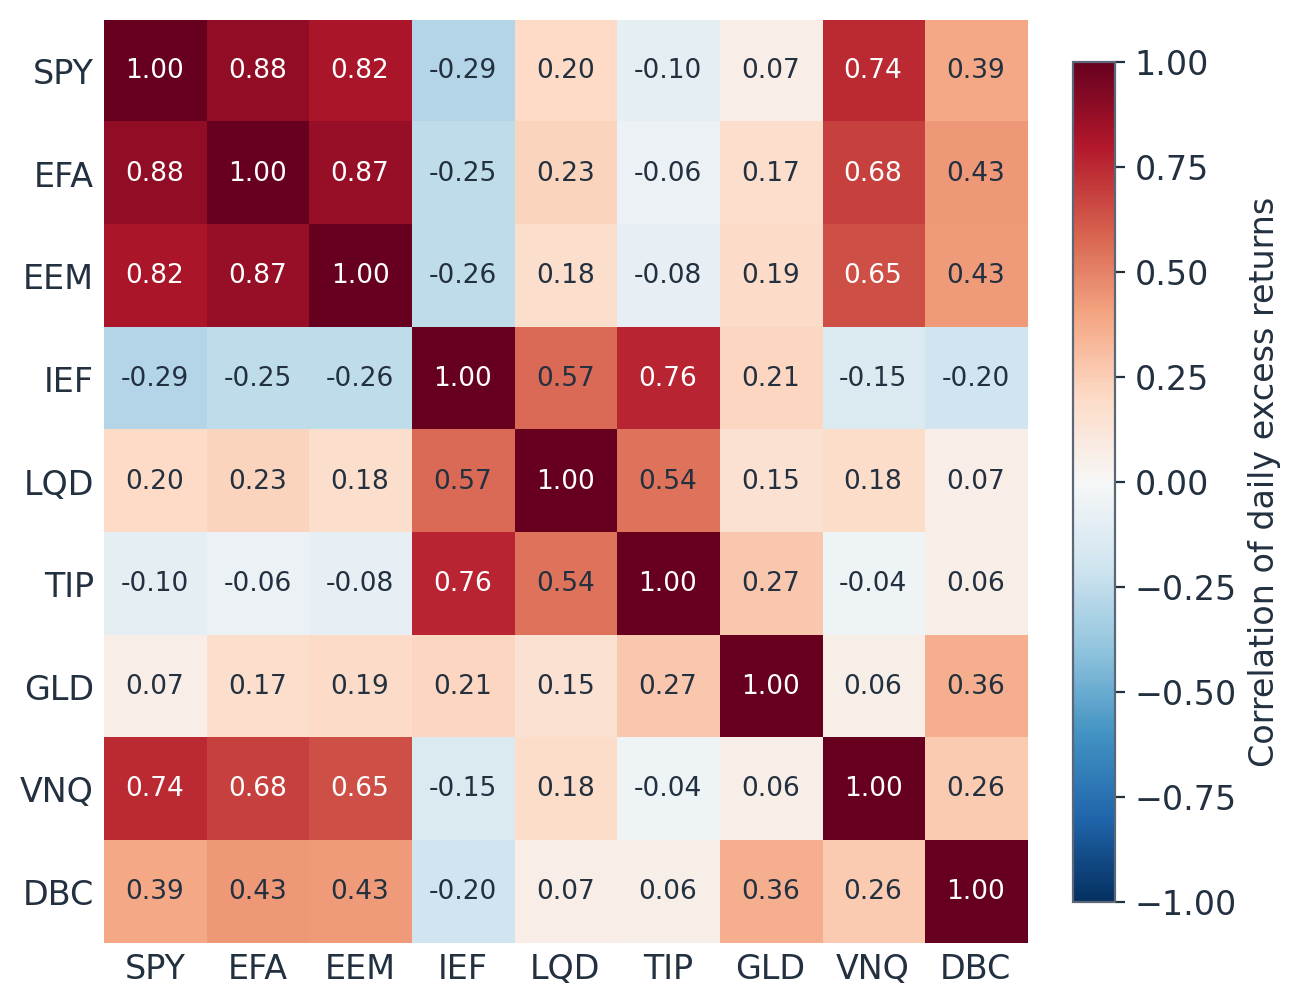
\includegraphics[width=0.62\linewidth,height=\textheight,keepaspectratio,alt={Figure A1. Correlation matrix of the nine ETFs' daily excess returns, 7 February 2006 to 31 July 2026.}]{figures/fig_correlation.png}
\caption{\textbf{Figure A1.} Correlation matrix of the nine ETFs' daily
excess returns, 7 February 2006 to 31 July 2026.}
\end{figure}

\begin{figure}
\centering
\pandocbounded{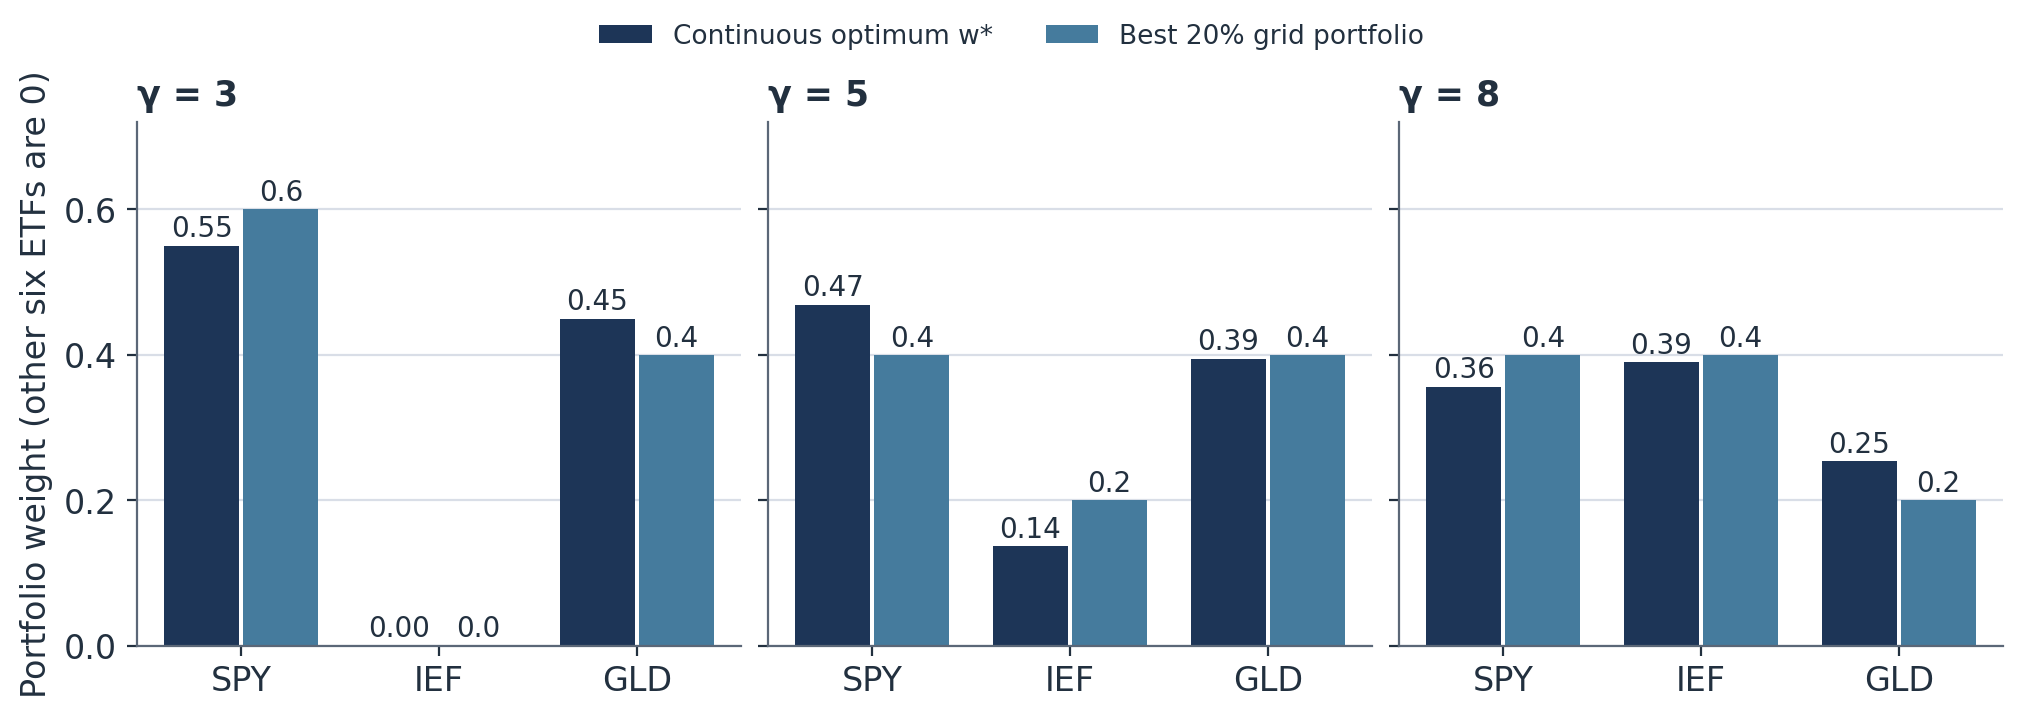
\includegraphics[keepaspectratio,alt={Figure A2. Continuous long-only optimum and best 20\% grid portfolio at each risk aversion. The six ETFs not shown have zero weight.}]{figures/fig_benchmarks_by_gamma.png}}
\caption{\textbf{Figure A2.} Continuous long-only optimum and best 20\%
grid portfolio at each risk aversion. The six ETFs not shown have zero
weight.}
\end{figure}

\begin{figure}
\centering
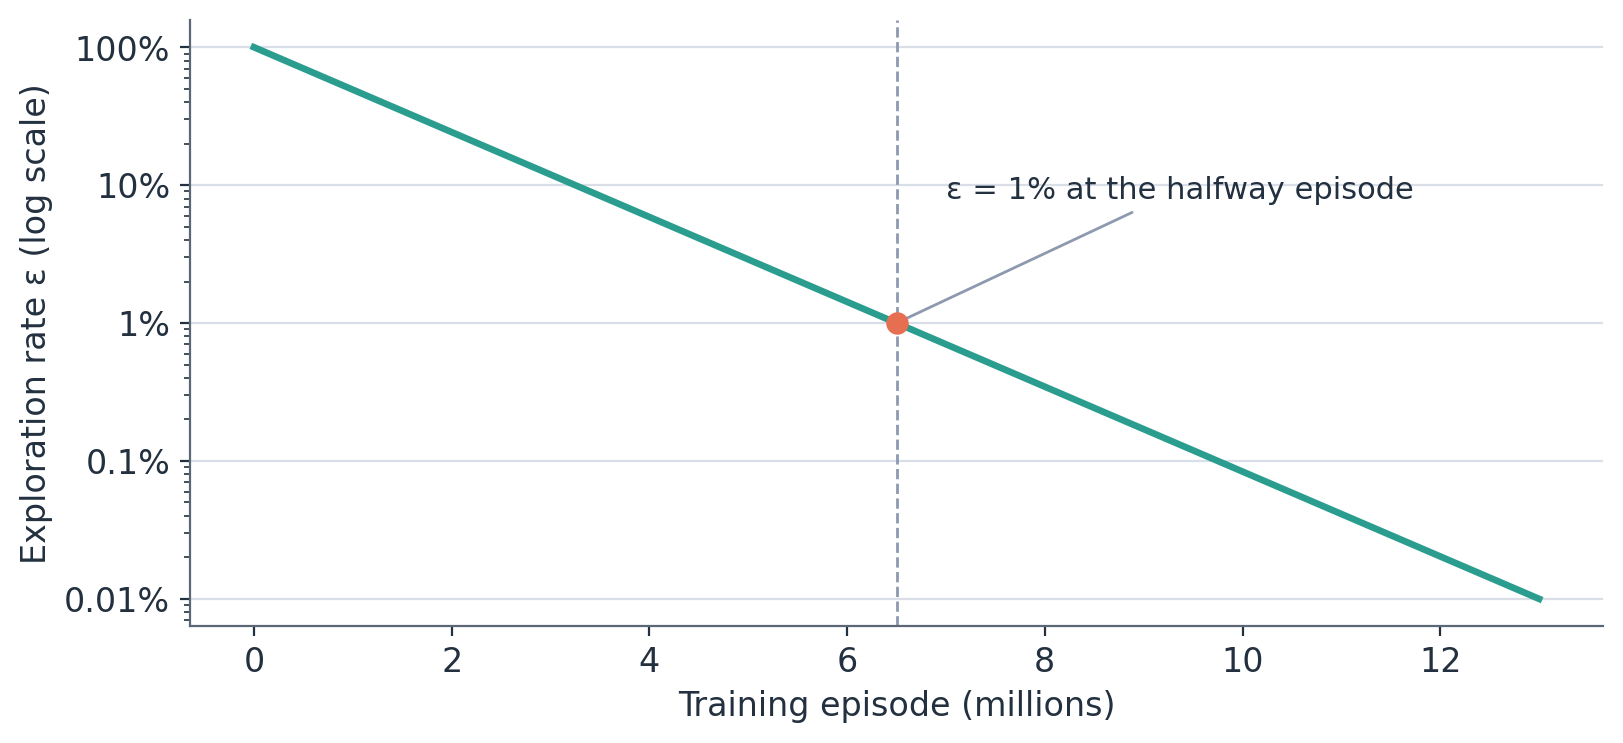
\includegraphics[width=0.75\linewidth,height=\textheight,keepaspectratio,alt={Figure A3. Exploration schedule of the pre-registered runs.}]{figures/fig_epsilon.png}
\caption{\textbf{Figure A3.} Exploration schedule of the pre-registered
runs.}
\end{figure}

\begin{figure}
\centering
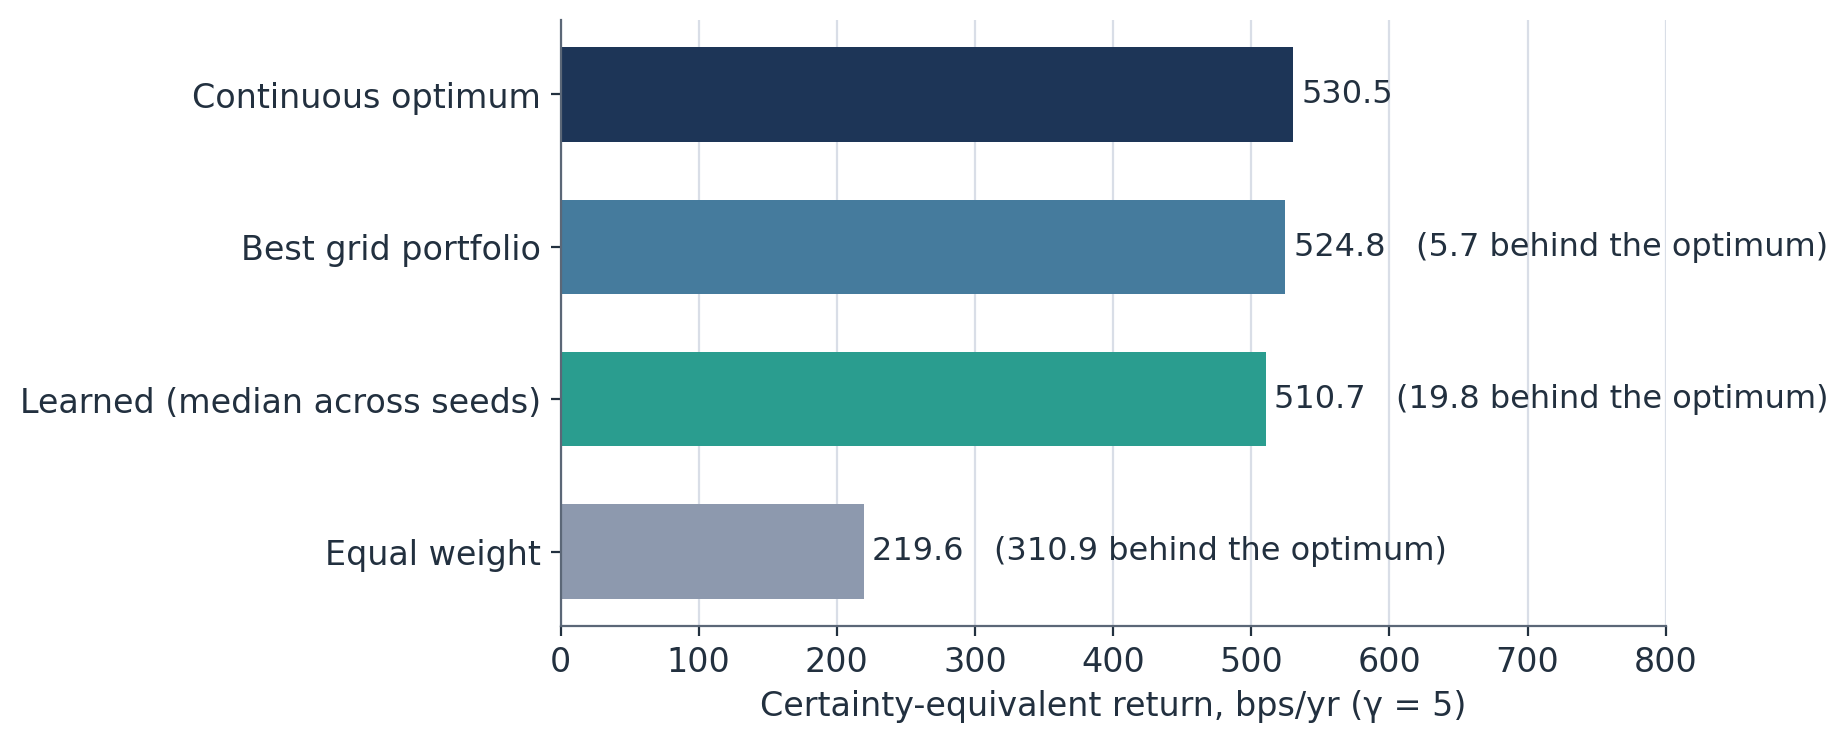
\includegraphics[width=0.85\linewidth,height=\textheight,keepaspectratio,alt={Figure A4. Certainty-equivalent return of the four portfolios at γ = 5 on the 20\% grid. The learned bar is the optimum minus the median total gap across seeds.}]{figures/fig_gap_ladder.png}
\caption{\textbf{Figure A4.} Certainty-equivalent return of the four
portfolios at γ = 5 on the 20\% grid. The learned bar is the optimum
minus the median total gap across seeds.}
\end{figure}

\begin{figure}
\centering
\pandocbounded{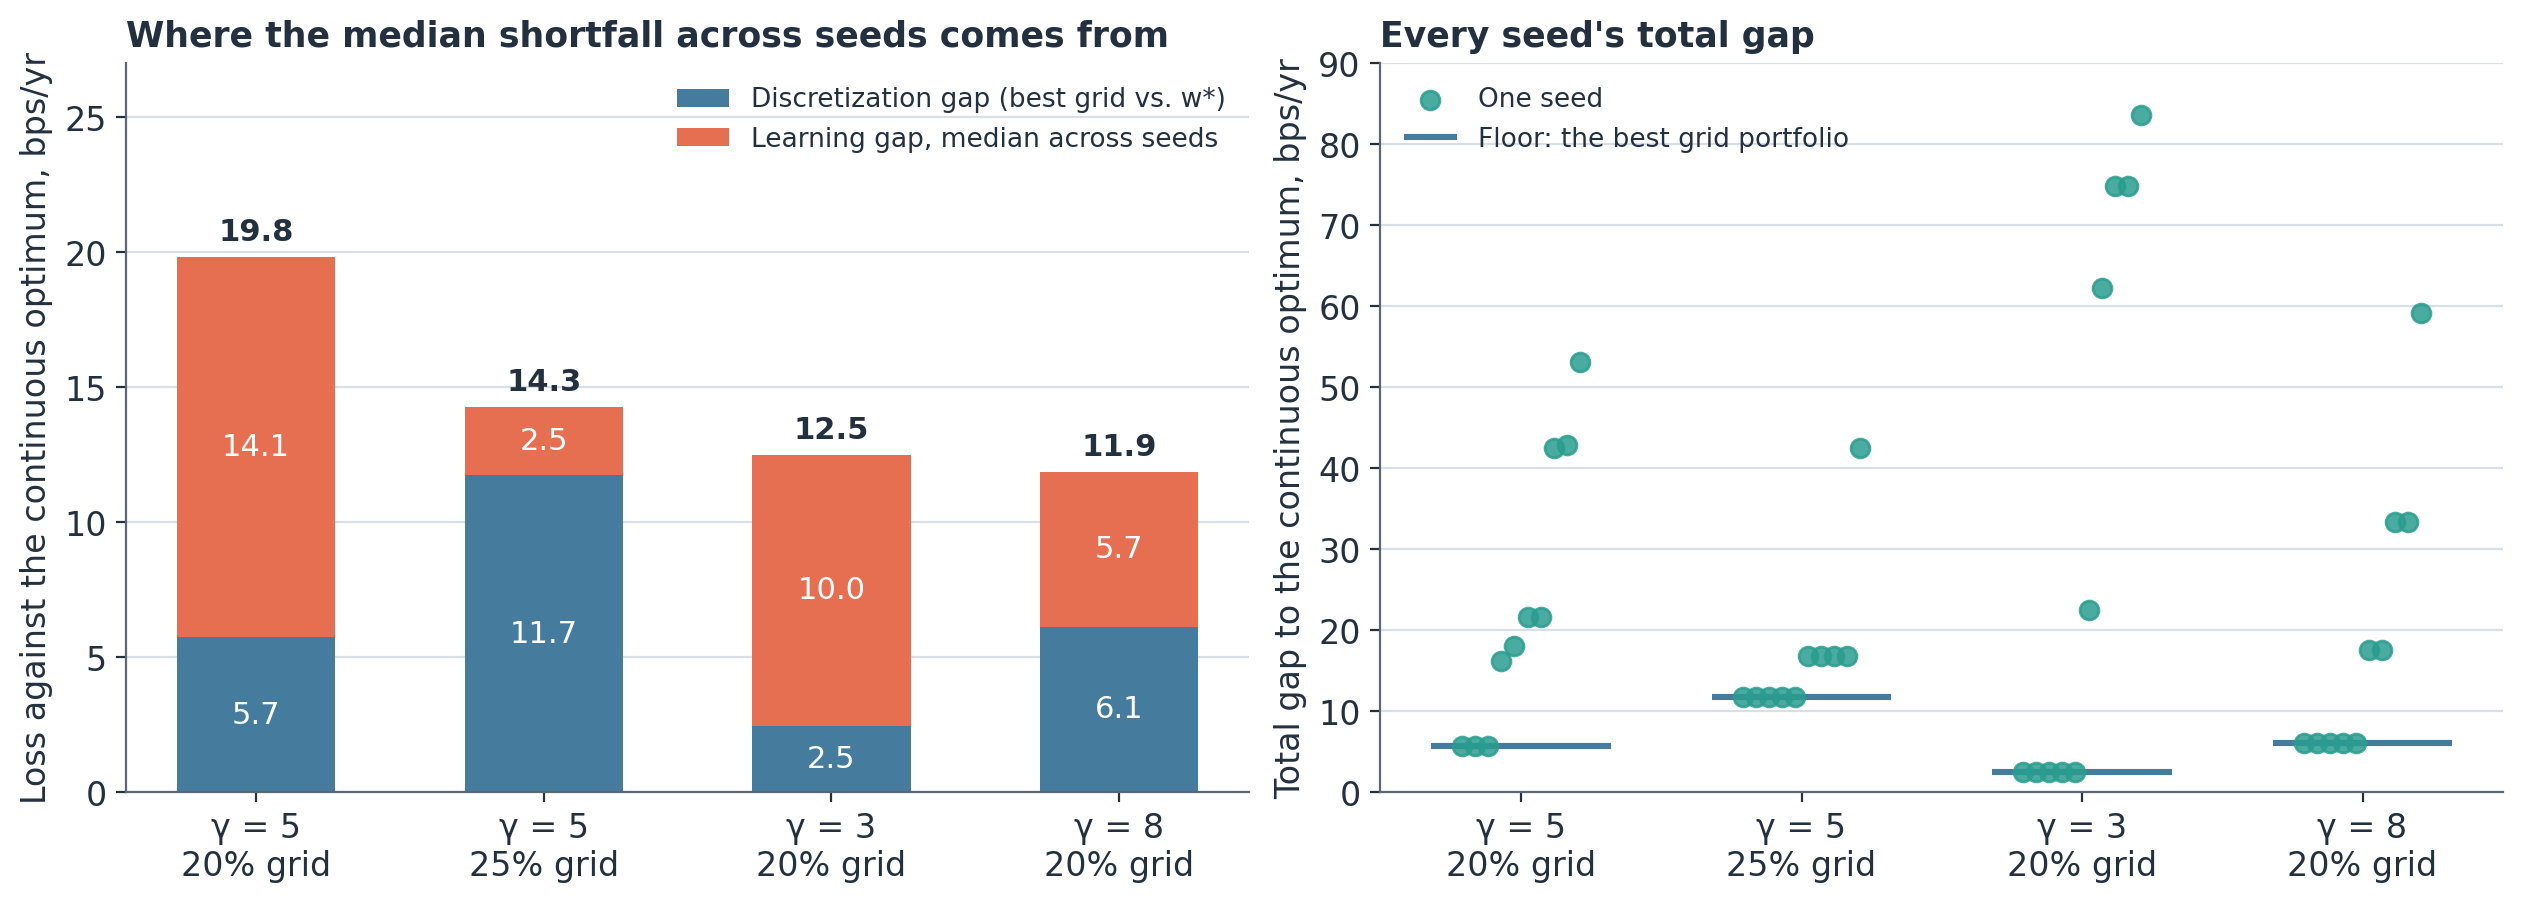
\includegraphics[keepaspectratio,alt={Figure A5. Left: the median shortfall across seeds against the continuous optimum, split into the discretization gap and the median learning gap. Right: every seed's total gap; seeds on the horizontal line found the best grid portfolio.}]{figures/fig_gaps.png}}
\caption{\textbf{Figure A5.} Left: the median shortfall across seeds
against the continuous optimum, split into the discretization gap and
the median learning gap. Right: every seed's total gap; seeds on the
horizontal line found the best grid portfolio.}
\end{figure}

\begin{figure}
\centering
\pandocbounded{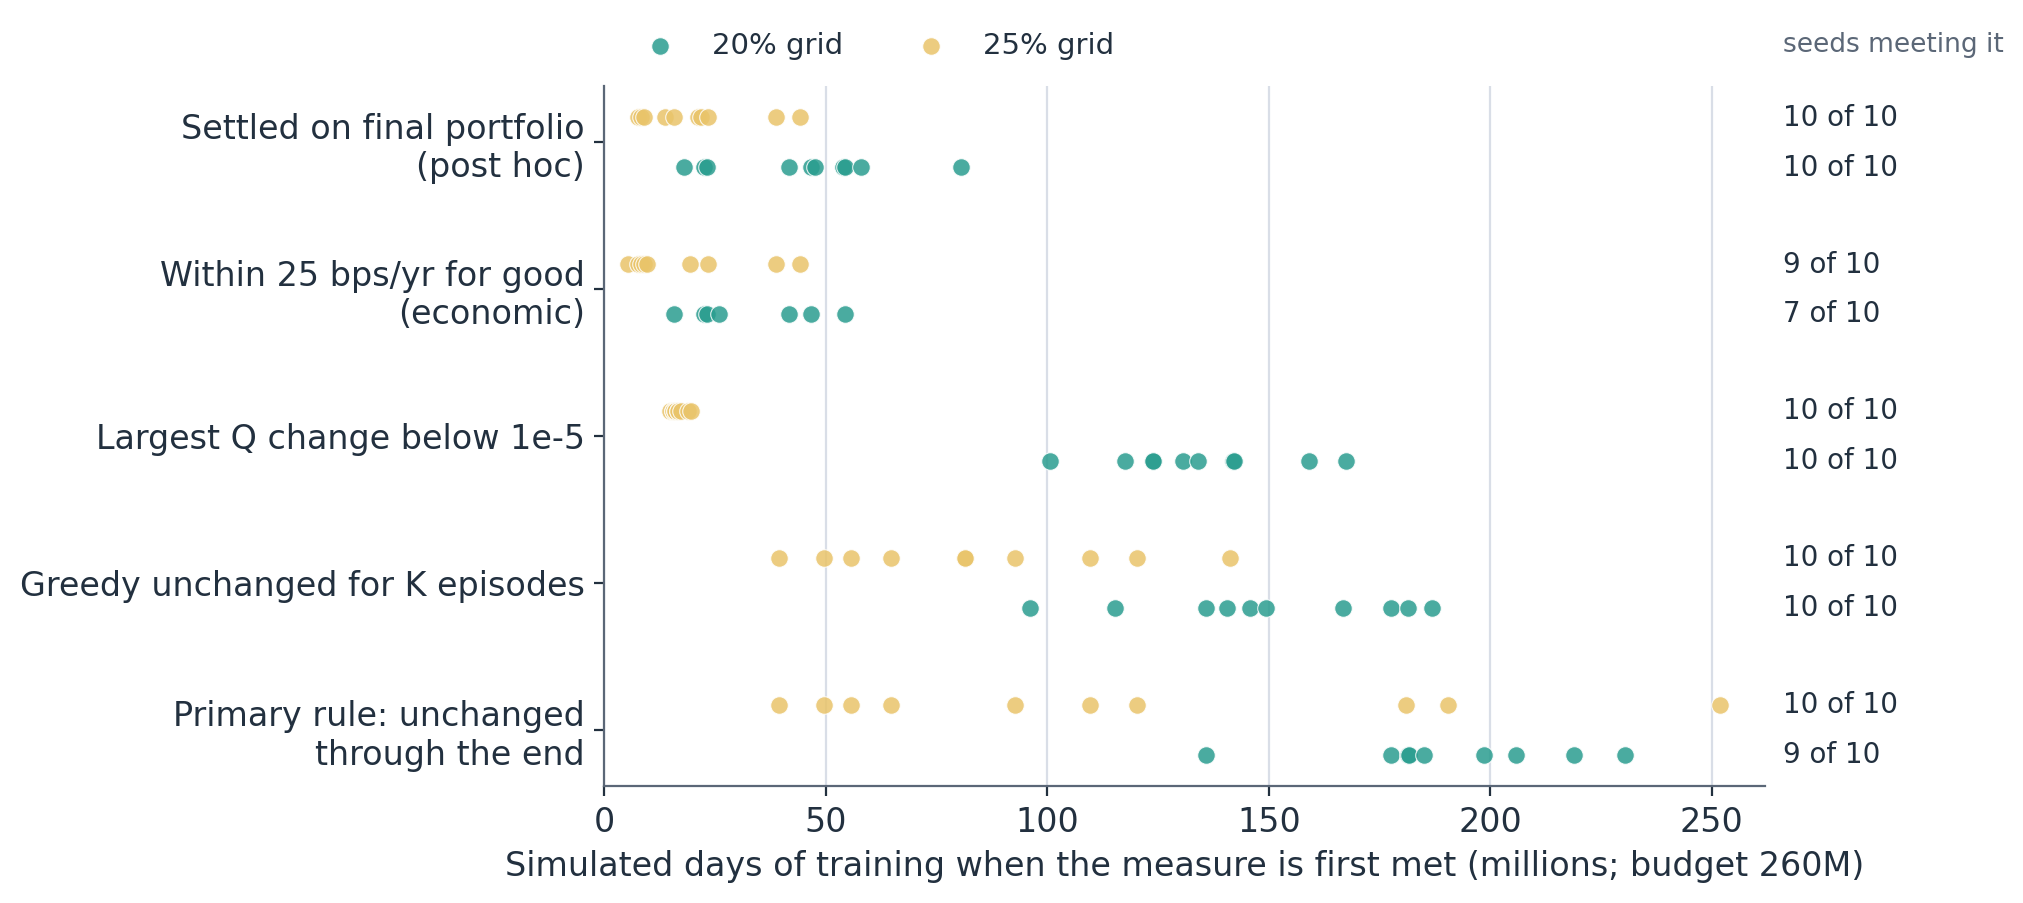
\includegraphics[keepaspectratio,alt={Figure A6. When each convergence measure is first met, one dot per seed, at γ = 5. ``Settled'' is the post hoc descriptive measure; the others were pre-registered.}]{figures/fig_convergence_times.png}}
\caption{\textbf{Figure A6.} When each convergence measure is first met,
one dot per seed, at γ = 5. ``Settled'' is the post hoc descriptive
measure; the others were pre-registered.}
\end{figure}

\begin{figure}
\centering
\pandocbounded{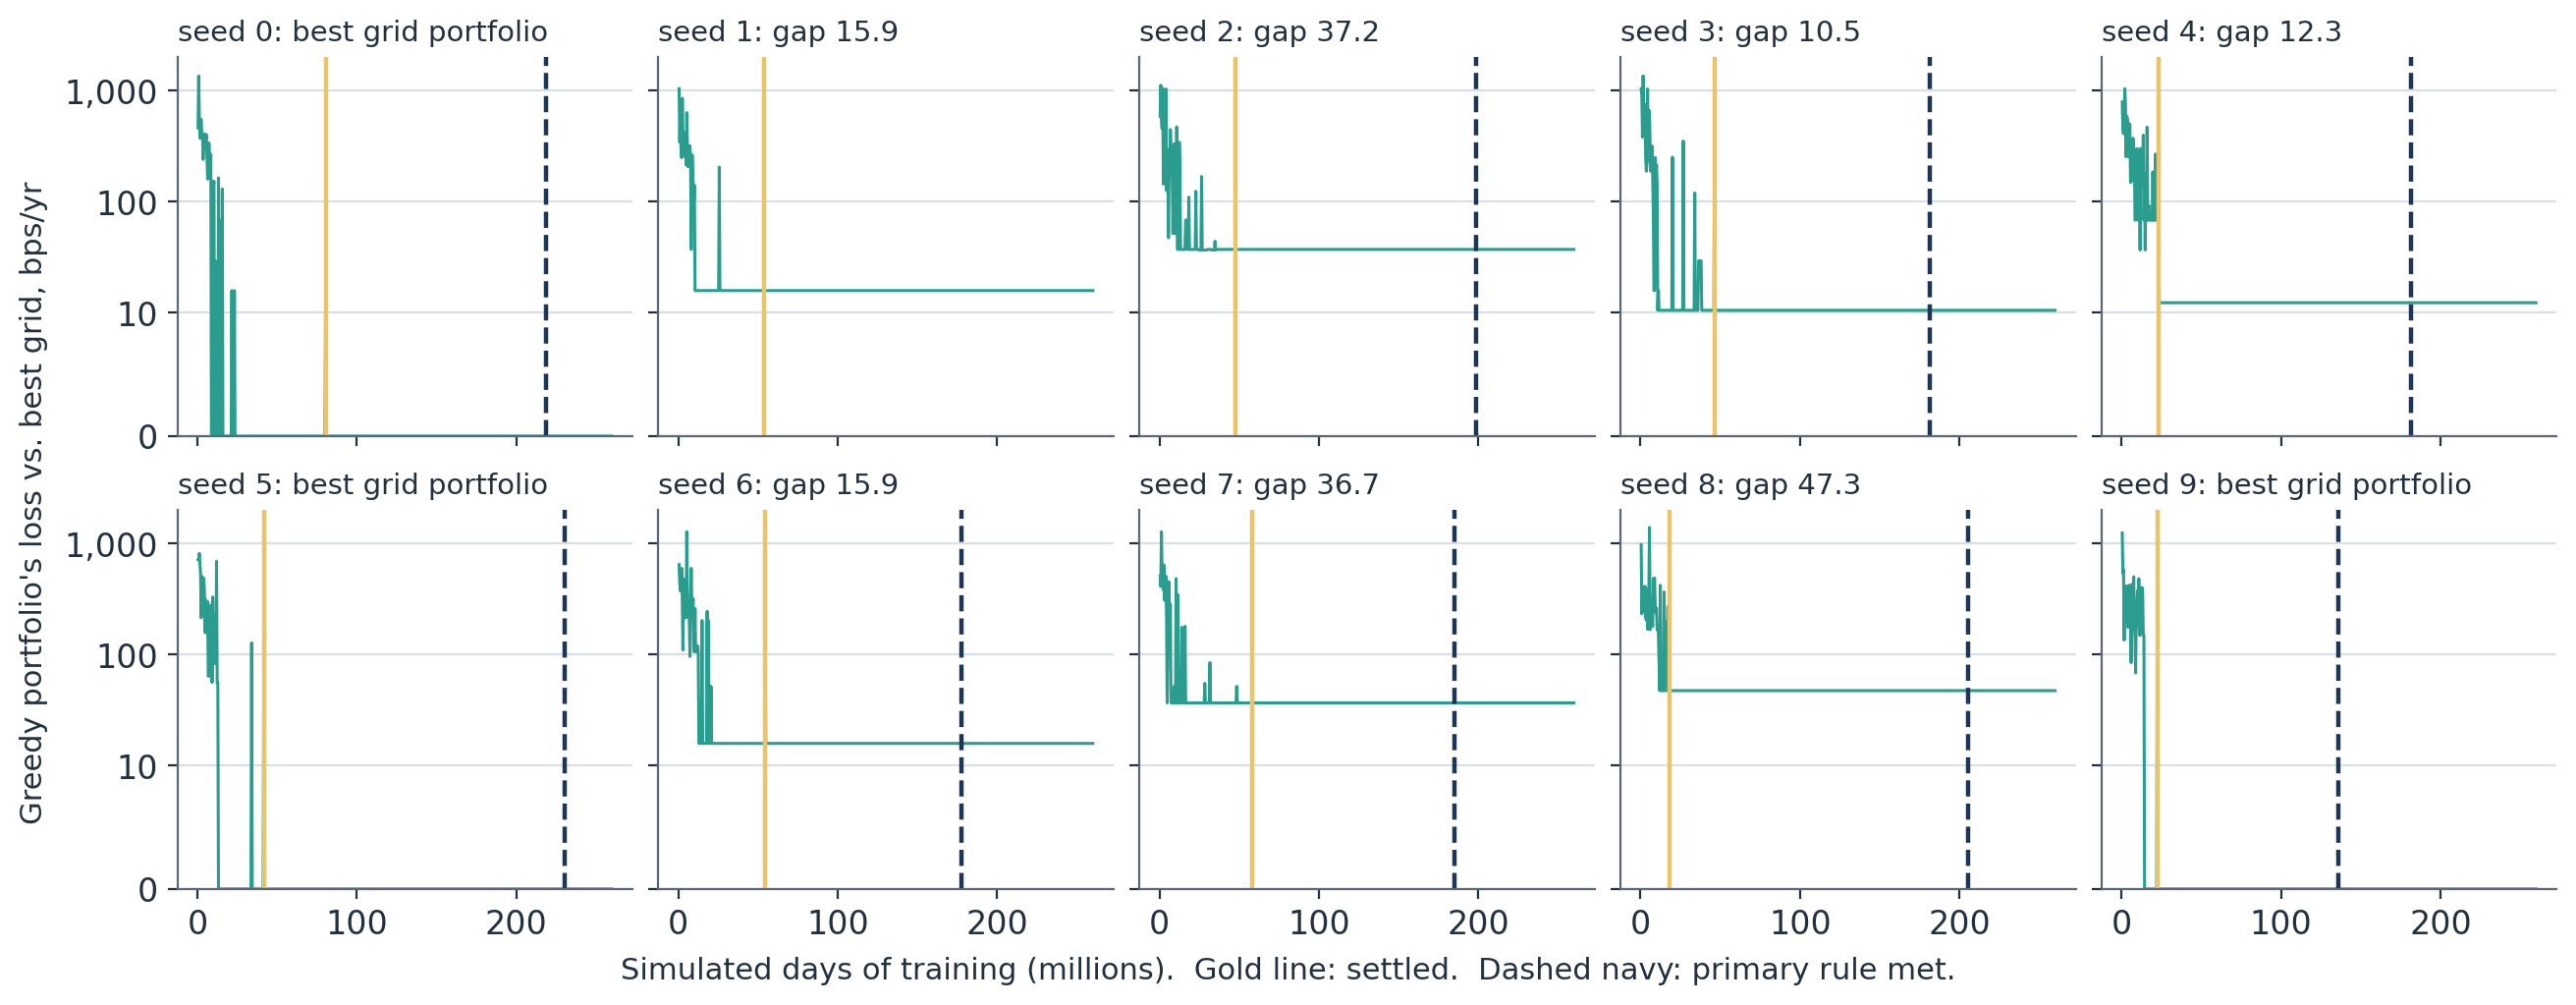
\includegraphics[keepaspectratio,alt={Figure A7. Loss of each seed's greedy portfolio during training (γ = 5, 20\% grid). Seed 1 does not meet the primary rule.}]{figures/fig_seed_paths.png}}
\caption{\textbf{Figure A7.} Loss of each seed's greedy portfolio during
training (γ = 5, 20\% grid). Seed 1 does not meet the primary rule.}
\end{figure}

\begin{figure}
\centering
\pandocbounded{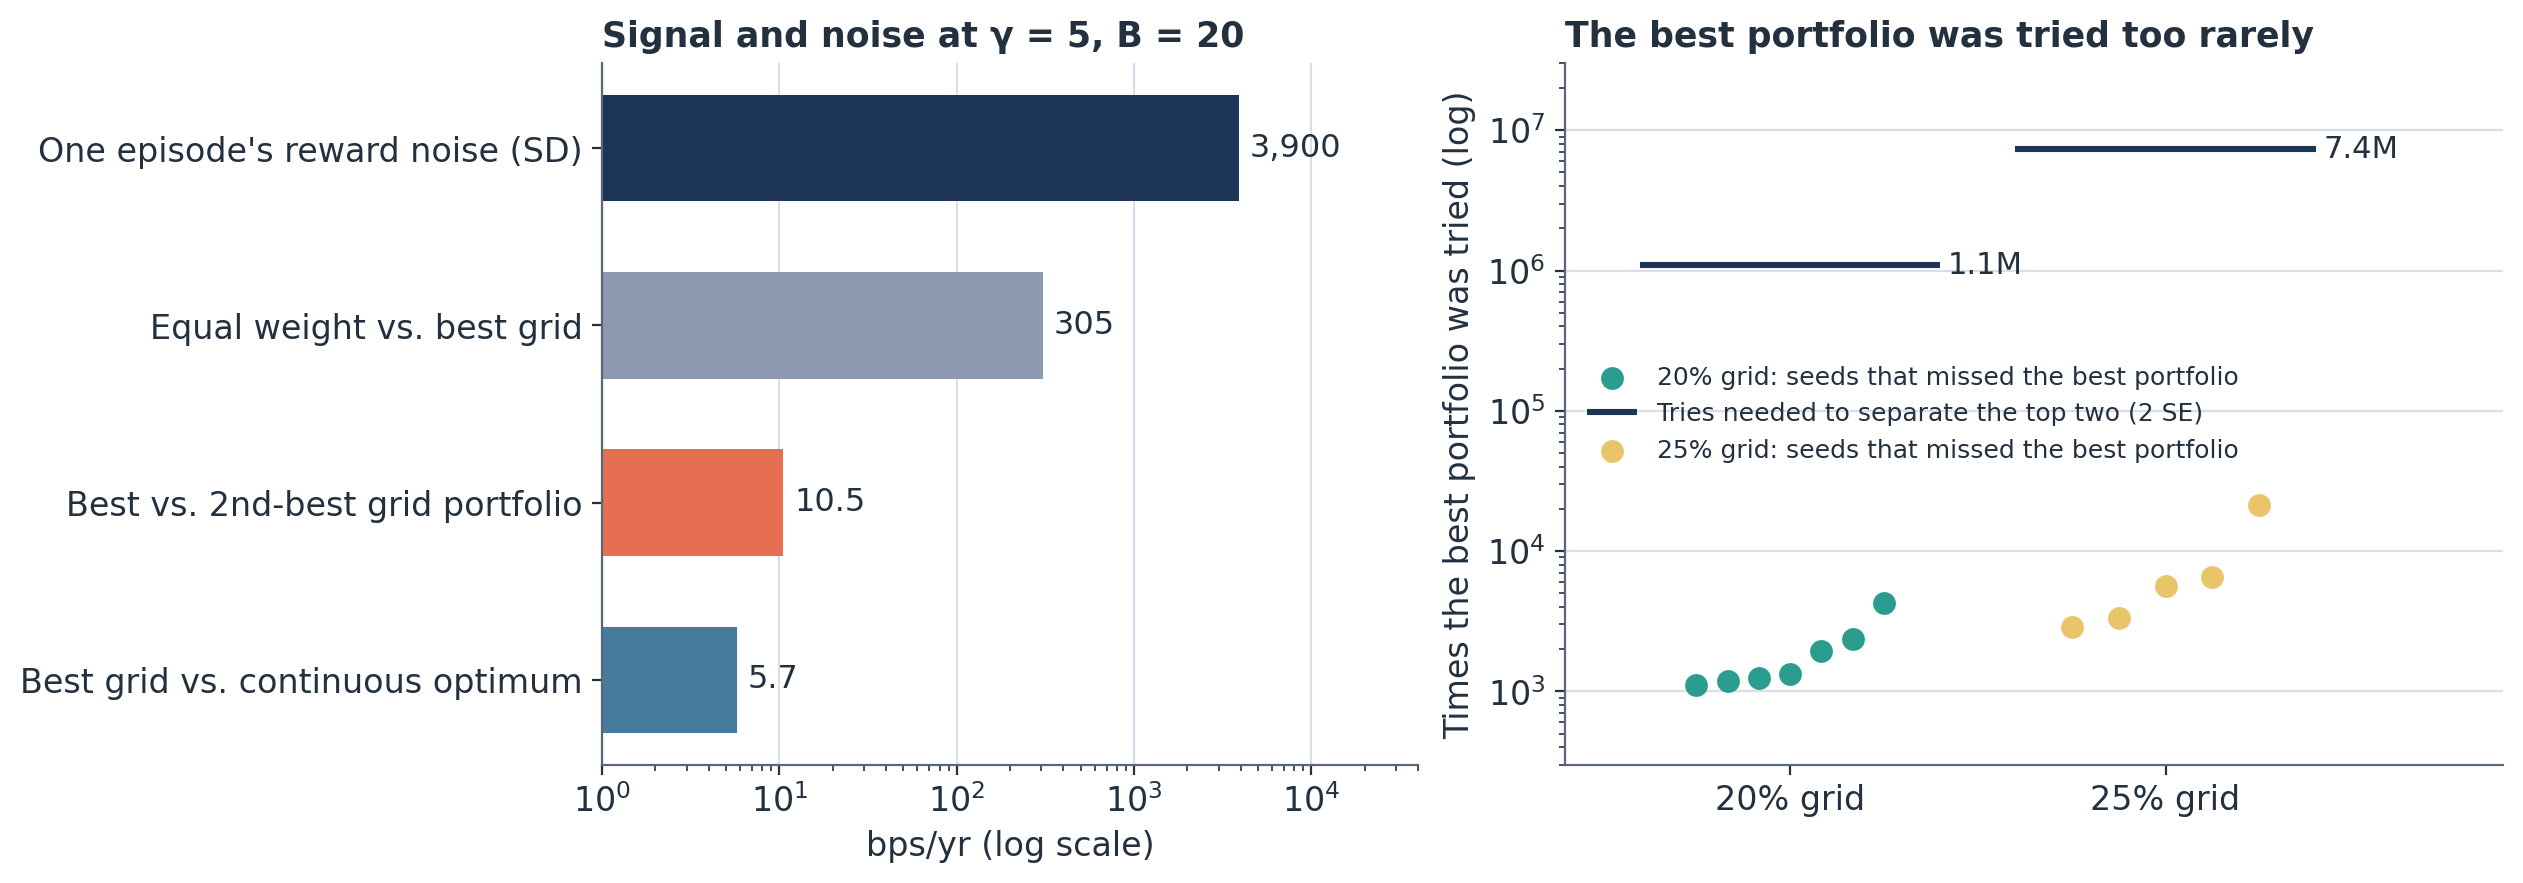
\includegraphics[keepaspectratio,alt={Figure A8. Left: one episode's reward noise against the utility differences the agent must detect (γ = 5, B = 20; logarithmic scale). Right: how often the best grid portfolio was tried in the seeds that did not select it, against the number of tries needed to separate it from the runner-up at two standard errors.}]{figures/fig_noise.png}}
\caption{\textbf{Figure A8.} Left: one episode's reward noise against
the utility differences the agent must detect (γ = 5, B = 20;
logarithmic scale). Right: how often the best grid portfolio was tried
in the seeds that did not select it, against the number of tries needed
to separate it from the runner-up at two standard errors.}
\end{figure}

\begin{figure}
\centering
\pandocbounded{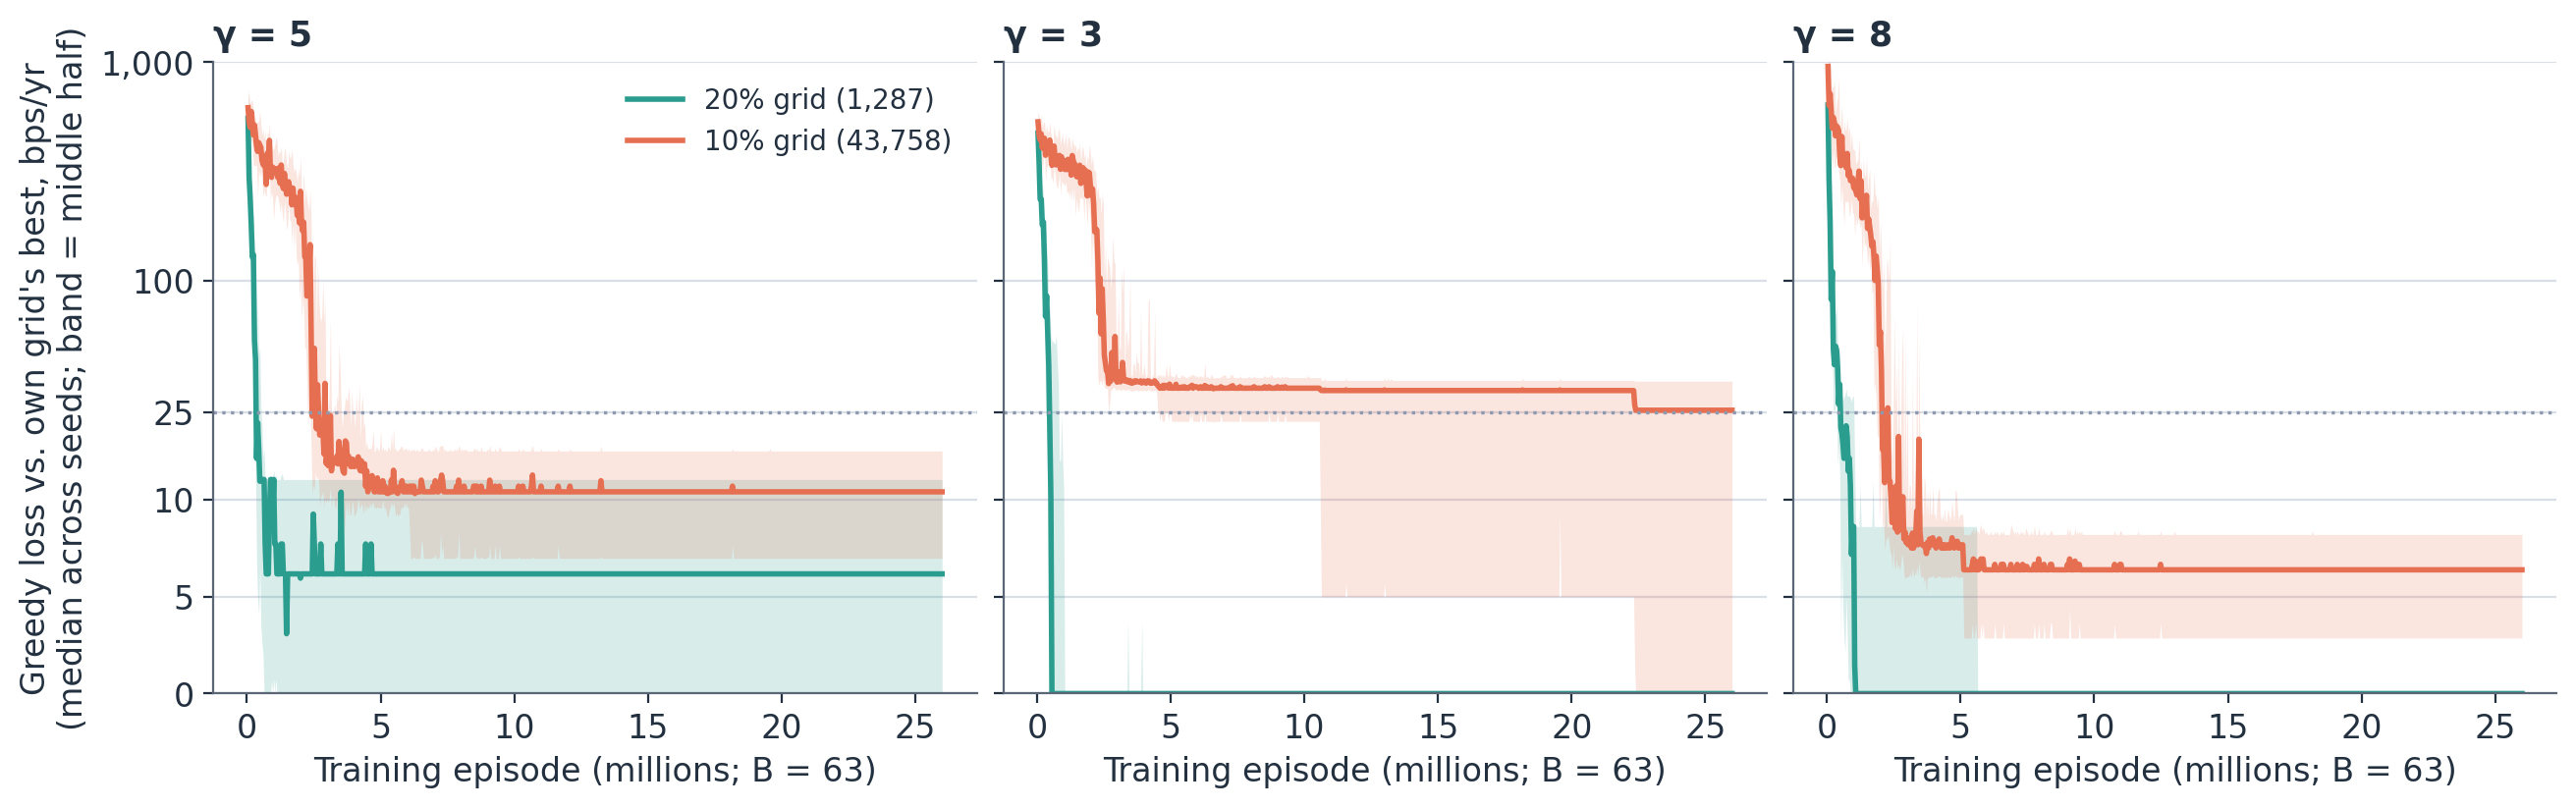
\includegraphics[keepaspectratio,alt={Figure A9. The 20\% and 10\% grids under identical settings at each γ (post hoc). Same construction as the right panel of Figure 3.}]{figures/fig_grid10.png}}
\caption{\textbf{Figure A9.} The 20\% and 10\% grids under identical
settings at each γ (post hoc). Same construction as the right panel of
Figure 3.}
\end{figure}

\begin{figure}
\centering
\pandocbounded{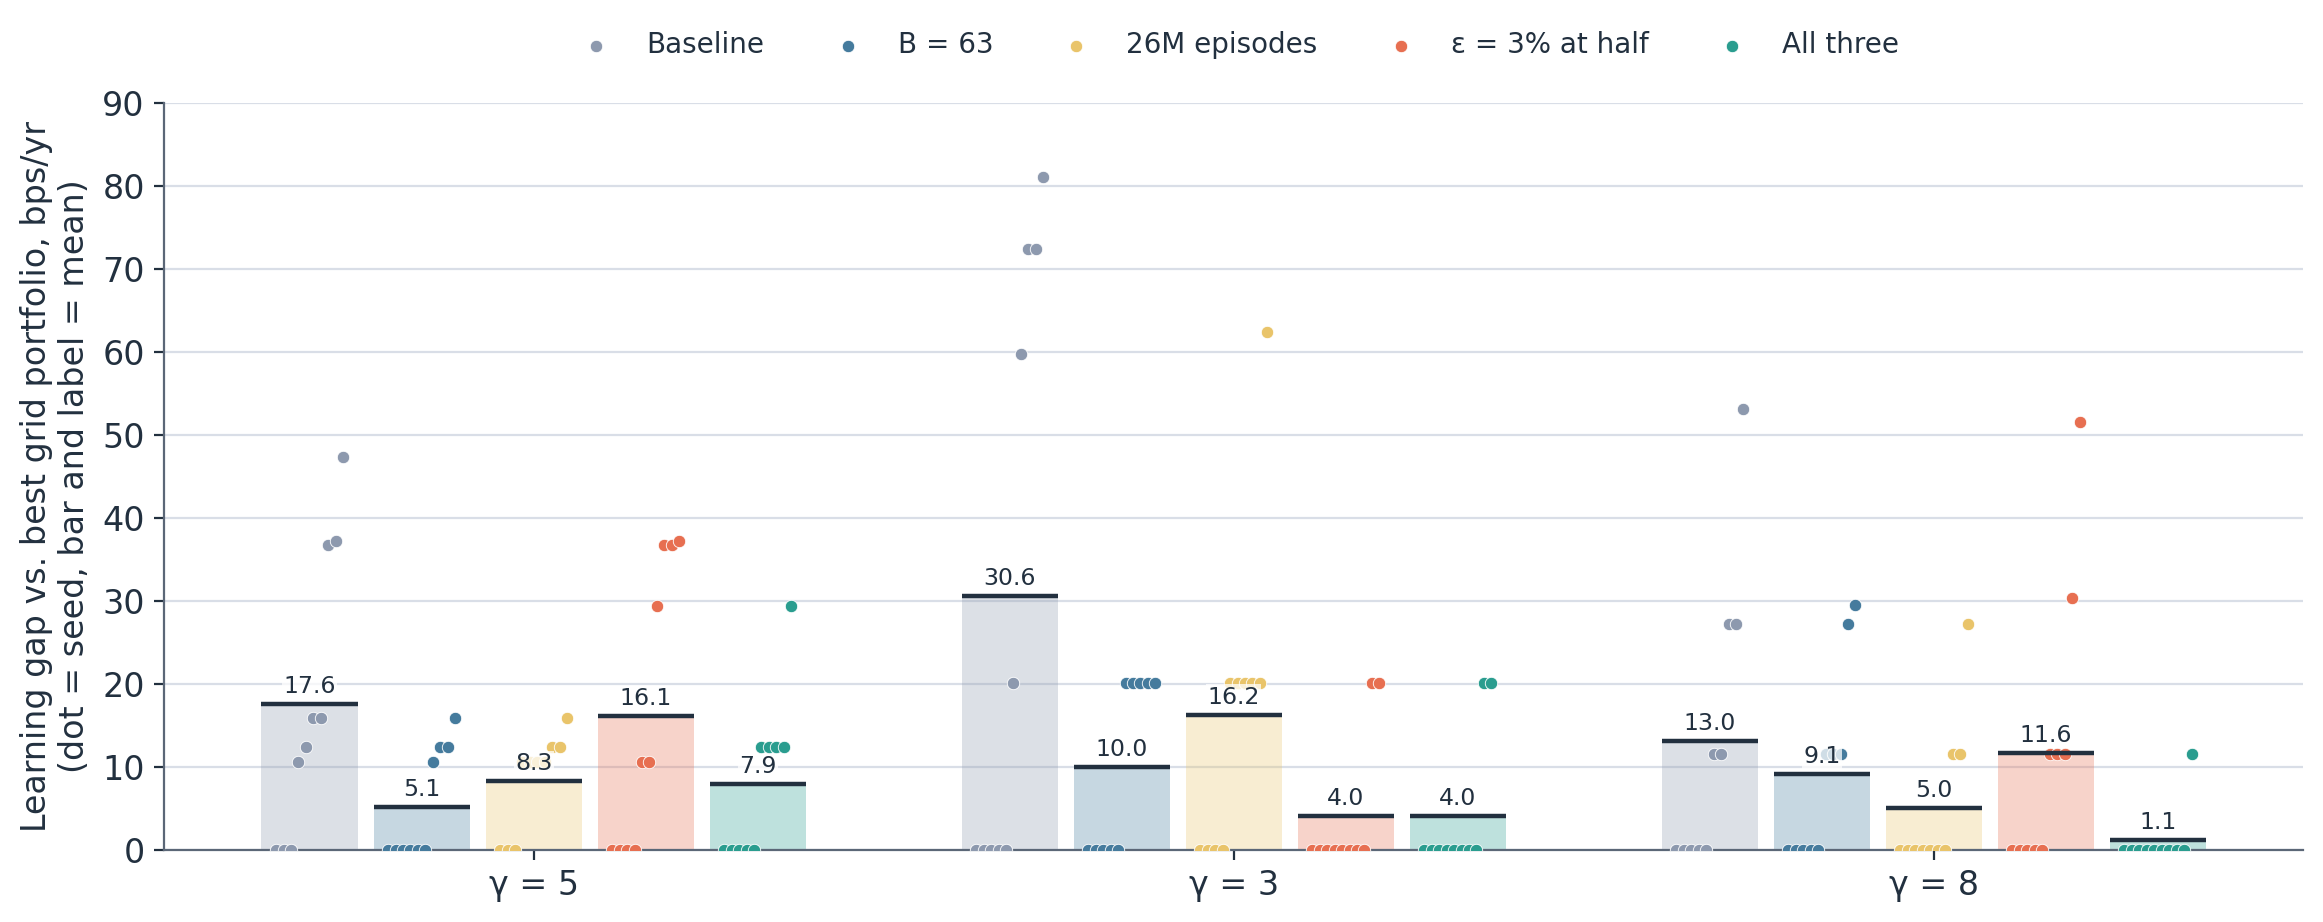
\includegraphics[keepaspectratio,alt={Figure A10. Learning gap for every seed (dots) and its mean (bar and label) under the baseline and the four post hoc tabular variants.}]{figures/fig_robustness.png}}
\caption{\textbf{Figure A10.} Learning gap for every seed (dots) and its
mean (bar and label) under the baseline and the four post hoc tabular
variants.}
\end{figure}

\begin{table}[htbp]
\centering\small
\caption{\textbf{Table A1.} How well each agent ranks the whole grid
(post hoc diagnostics). Medians over ten seeds at γ = 5 / 3 /
8.}
\begin{tabular}{@{}
  >{\raggedright\arraybackslash}p{(\linewidth - 8\tabcolsep) * \real{0.2000}}
  >{\raggedright\arraybackslash}p{(\linewidth - 8\tabcolsep) * \real{0.2000}}
  >{\raggedright\arraybackslash}p{(\linewidth - 8\tabcolsep) * \real{0.2000}}
  >{\raggedright\arraybackslash}p{(\linewidth - 8\tabcolsep) * \real{0.2000}}
  >{\raggedright\arraybackslash}p{(\linewidth - 8\tabcolsep) * \real{0.2000}}@{}}
\toprule\noalign{}
\begin{minipage}[b]{\linewidth}\raggedright
Run
\end{minipage} & \begin{minipage}[b]{\linewidth}\raggedright
Spearman correlation with true utility
\end{minipage} & \begin{minipage}[b]{\linewidth}\raggedright
True top ten found
\end{minipage} & \begin{minipage}[b]{\linewidth}\raggedright
Exactly best (of 10)
\end{minipage} & \begin{minipage}[b]{\linewidth}\raggedright
Primary rule met (of 10)
\end{minipage} \\
\midrule\noalign{}
Table, α = 1/N (baseline) & 0.821 / 0.710 / 0.920 & 35\% / 20\% / 20\% &
3 / 5 / 5 & 9 / 8 / 9 \\
Table, constant α & 0.813 / 0.703 / 0.917 & 25\% / 15\% / 20\% & 0 / 2 /
0 & 10 / 8 / 10 \\
Quadratic features & 0.915 / 0.854 / 0.951 & 55\% / 80\% / 20\% & 0 / 6
/ 0 & 2 / 0 / 9 \\
Splines & 0.950 / 0.945 / 0.957 & 45\% / 65\% / 20\% & 5 / 3 / 0 & 10 /
10 / 9 \\
10\% grid, table & 0.543 / 0.406 / 0.725 & 10\% / 10\% / 10\% & 0 / 4 /
1 & 0 / 0 / 0 \\
10\% grid, splines, ε 3\% & 0.976 / 0.963 / 0.983 & 0\% / 0\% / 10\% & 0
/ 0 / 0 & 0 / 0 / 0 \\
10\% grid, splines, ε 10\% & 0.975 / 0.964 / 0.985 & 0\% / 0\% / 0\% & 0
/ 0 / 0 & 0 / 0 / 0 \\
\bottomrule\noalign{}
\end{tabular}
\end{table}

\begin{figure}
\centering
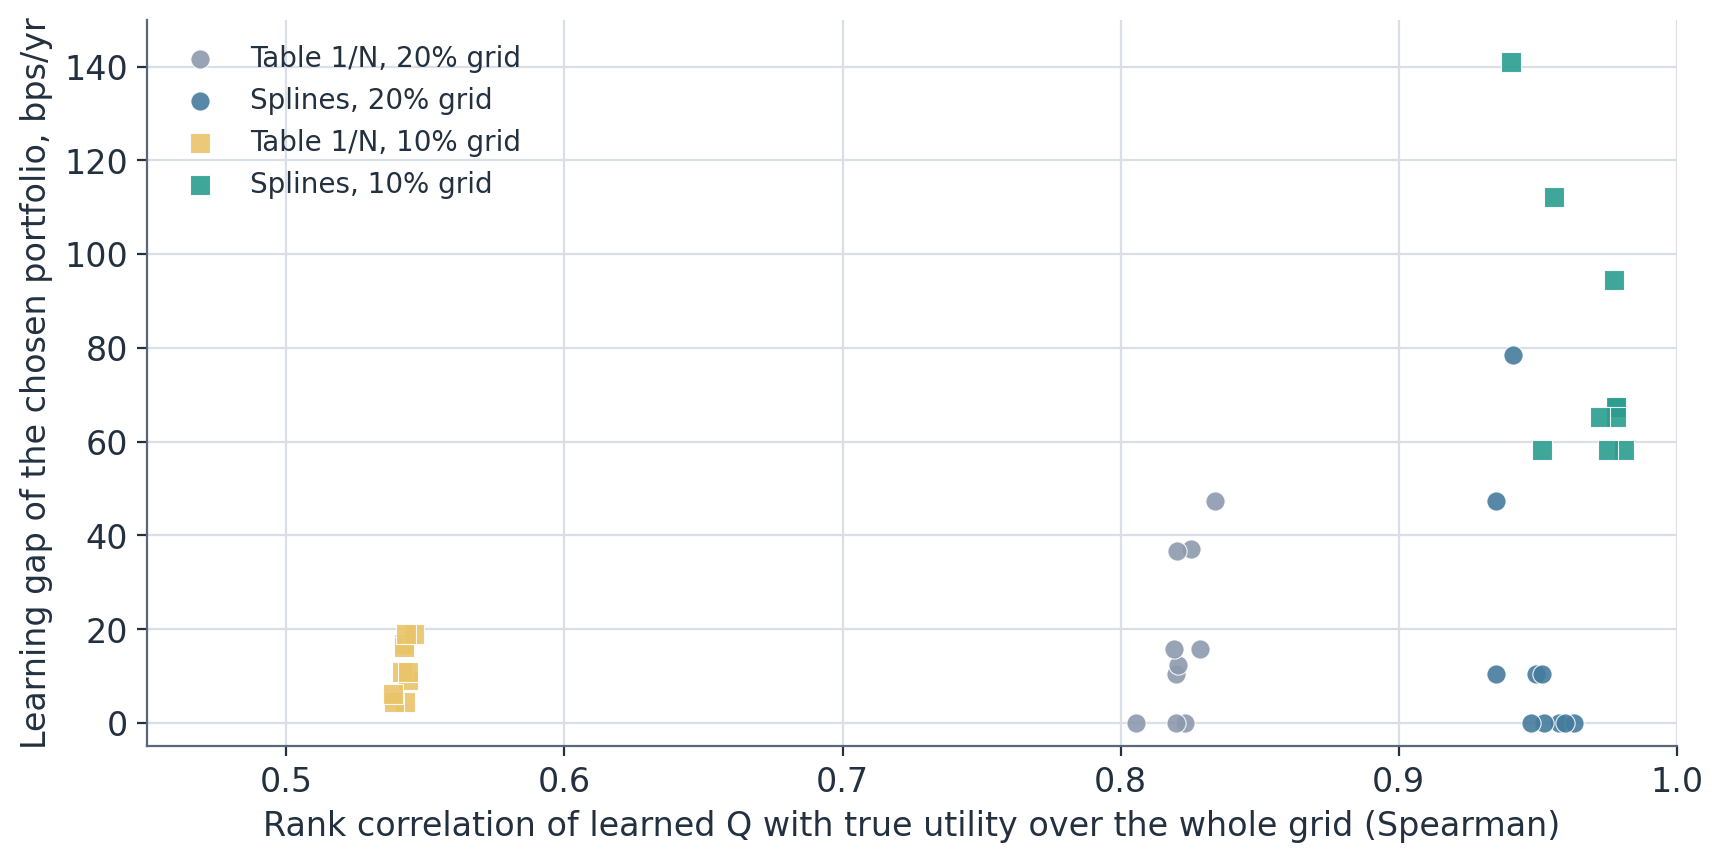
\includegraphics[width=0.8\linewidth,height=\textheight,keepaspectratio,alt={Figure A11. Overall ranking quality against the quality of the chosen portfolio, one marker per seed at γ = 5. Splines on the 10\% grid rank the grid best and choose worst.}]{figures/fig_fa_ranking.png}
\caption{\textbf{Figure A11.} Overall ranking quality against the
quality of the chosen portfolio, one marker per seed at γ = 5. Splines
on the 10\% grid rank the grid best and choose worst.}
\end{figure}

\begin{table}[htbp]
\centering\small
\caption{\textbf{Table A2.} First transaction-cost design (negative
result). Expected net certainty equivalent, bps/yr, by the cost of a
20-point transfer between two ETFs. Ten seeds.}
\begin{tabular}{@{}
  >{\raggedright\arraybackslash}p{(\linewidth - 10\tabcolsep) * \real{0.1304}}
  >{\raggedleft\arraybackslash}p{(\linewidth - 10\tabcolsep) * \real{0.1739}}
  >{\raggedleft\arraybackslash}p{(\linewidth - 10\tabcolsep) * \real{0.1739}}
  >{\raggedleft\arraybackslash}p{(\linewidth - 10\tabcolsep) * \real{0.1739}}
  >{\raggedleft\arraybackslash}p{(\linewidth - 10\tabcolsep) * \real{0.1739}}
  >{\raggedleft\arraybackslash}p{(\linewidth - 10\tabcolsep) * \real{0.1739}}@{}}
\toprule\noalign{}
\begin{minipage}[b]{\linewidth}\raggedright
Cost
\end{minipage} & \begin{minipage}[b]{\linewidth}\raggedleft
Grid oracle
\end{minipage} & \begin{minipage}[b]{\linewidth}\raggedleft
Ignore costs
\end{minipage} & \begin{minipage}[b]{\linewidth}\raggedleft
Myopic
\end{minipage} & \begin{minipage}[b]{\linewidth}\raggedleft
Learned (median)
\end{minipage} & \begin{minipage}[b]{\linewidth}\raggedleft
Learned gap to oracle, median (range)
\end{minipage} \\
\midrule\noalign{}
0 bp & 524.8 & 524.8 & 524.8 & 56.6 & 468.2 (436.4 to 485.2) \\
1 bp & 520.9 & 520.8 & 515.9 & −16.8 & 537.7 (482.4 to 589.8) \\
2 bp & 517.1 & 516.8 & 512.6 & −90.9 & 608.0 (572.5 to 658.7) \\
5 bp & 507.6 & 504.9 & 479.2 & −296.8 & 804.3 (744.9 to 844.3) \\
\bottomrule\noalign{}
\end{tabular}
\end{table}

\begin{figure}
\centering
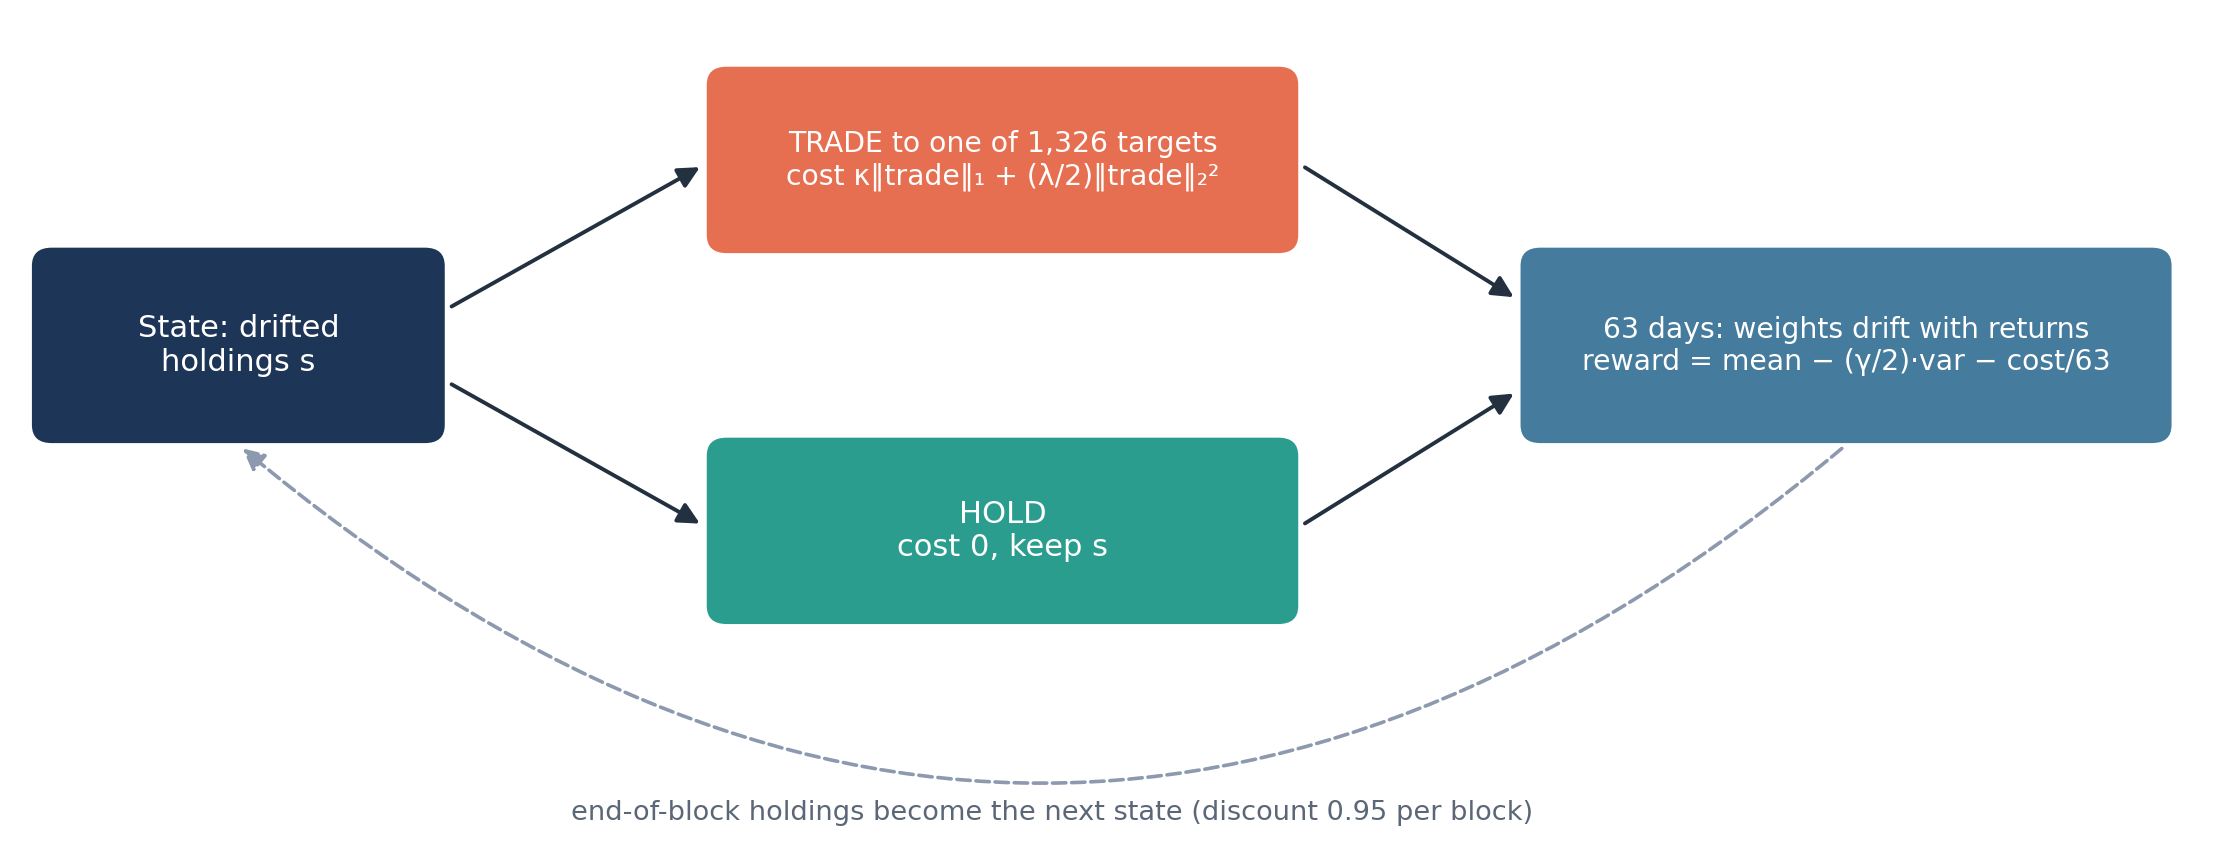
\includegraphics[width=0.85\linewidth,height=\textheight,keepaspectratio,alt={Figure A12. One block of the redesigned transaction-cost problem.}]{figures/fig_tc_schematic.png}
\caption{\textbf{Figure A12.} One block of the redesigned
transaction-cost problem.}
\end{figure}

\begin{figure}
\centering
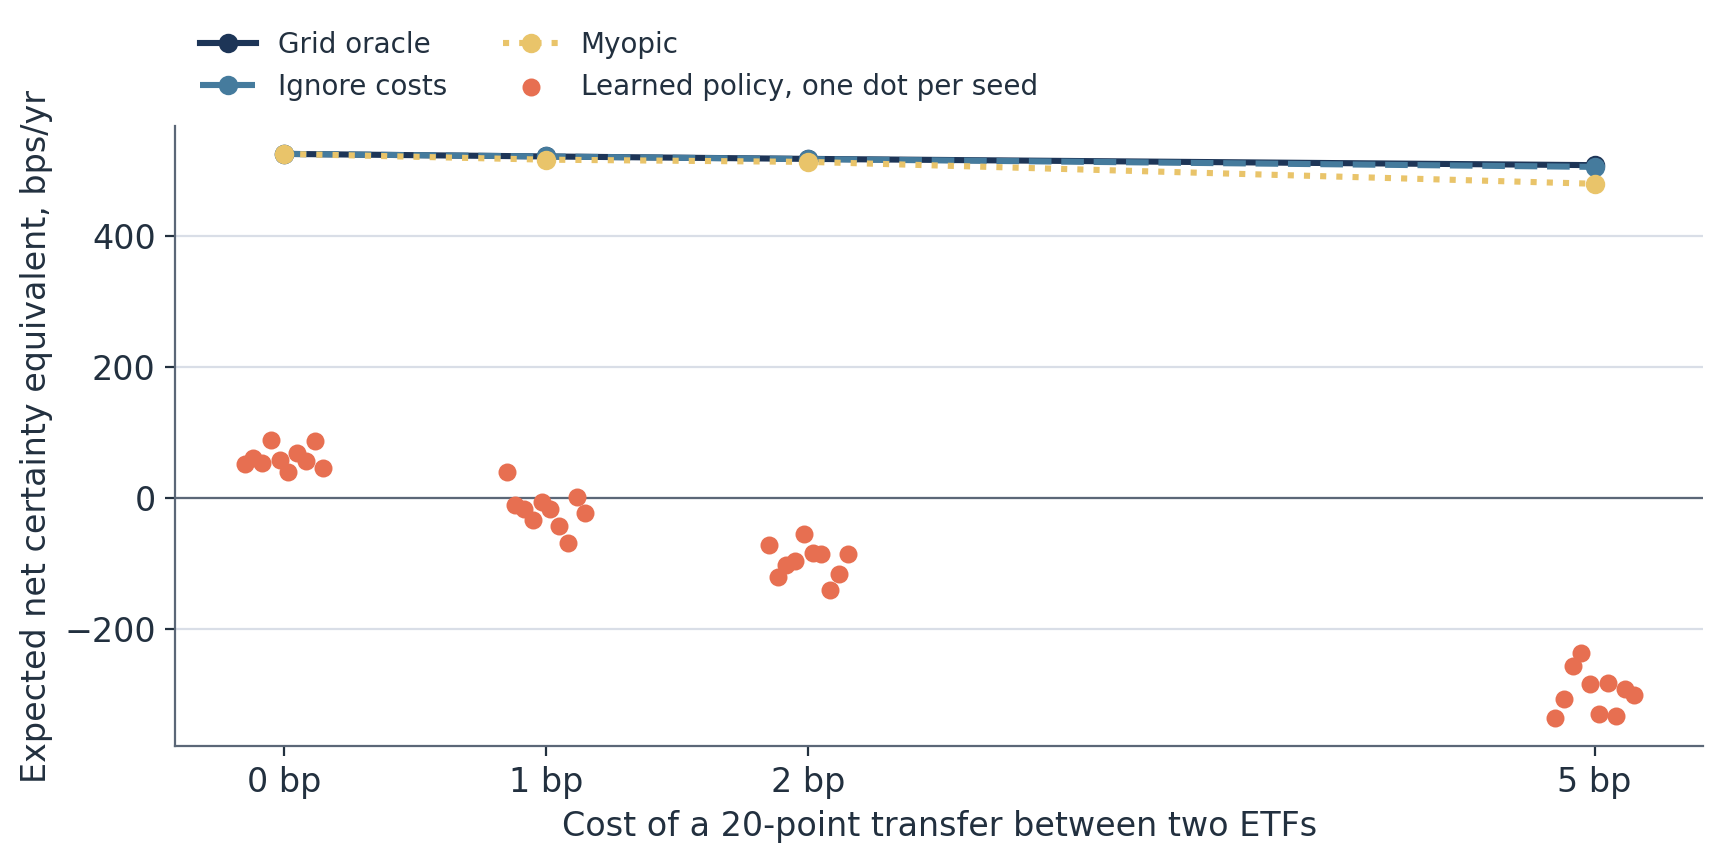
\includegraphics[width=0.75\linewidth,height=\textheight,keepaspectratio,alt={Figure A13. First transaction-cost design: the learned policies against their benchmarks.}]{figures/fig_tc_first_design.png}
\caption{\textbf{Figure A13.} First transaction-cost design: the learned
policies against their benchmarks.}
\end{figure}

\begin{figure}
\centering
\pandocbounded{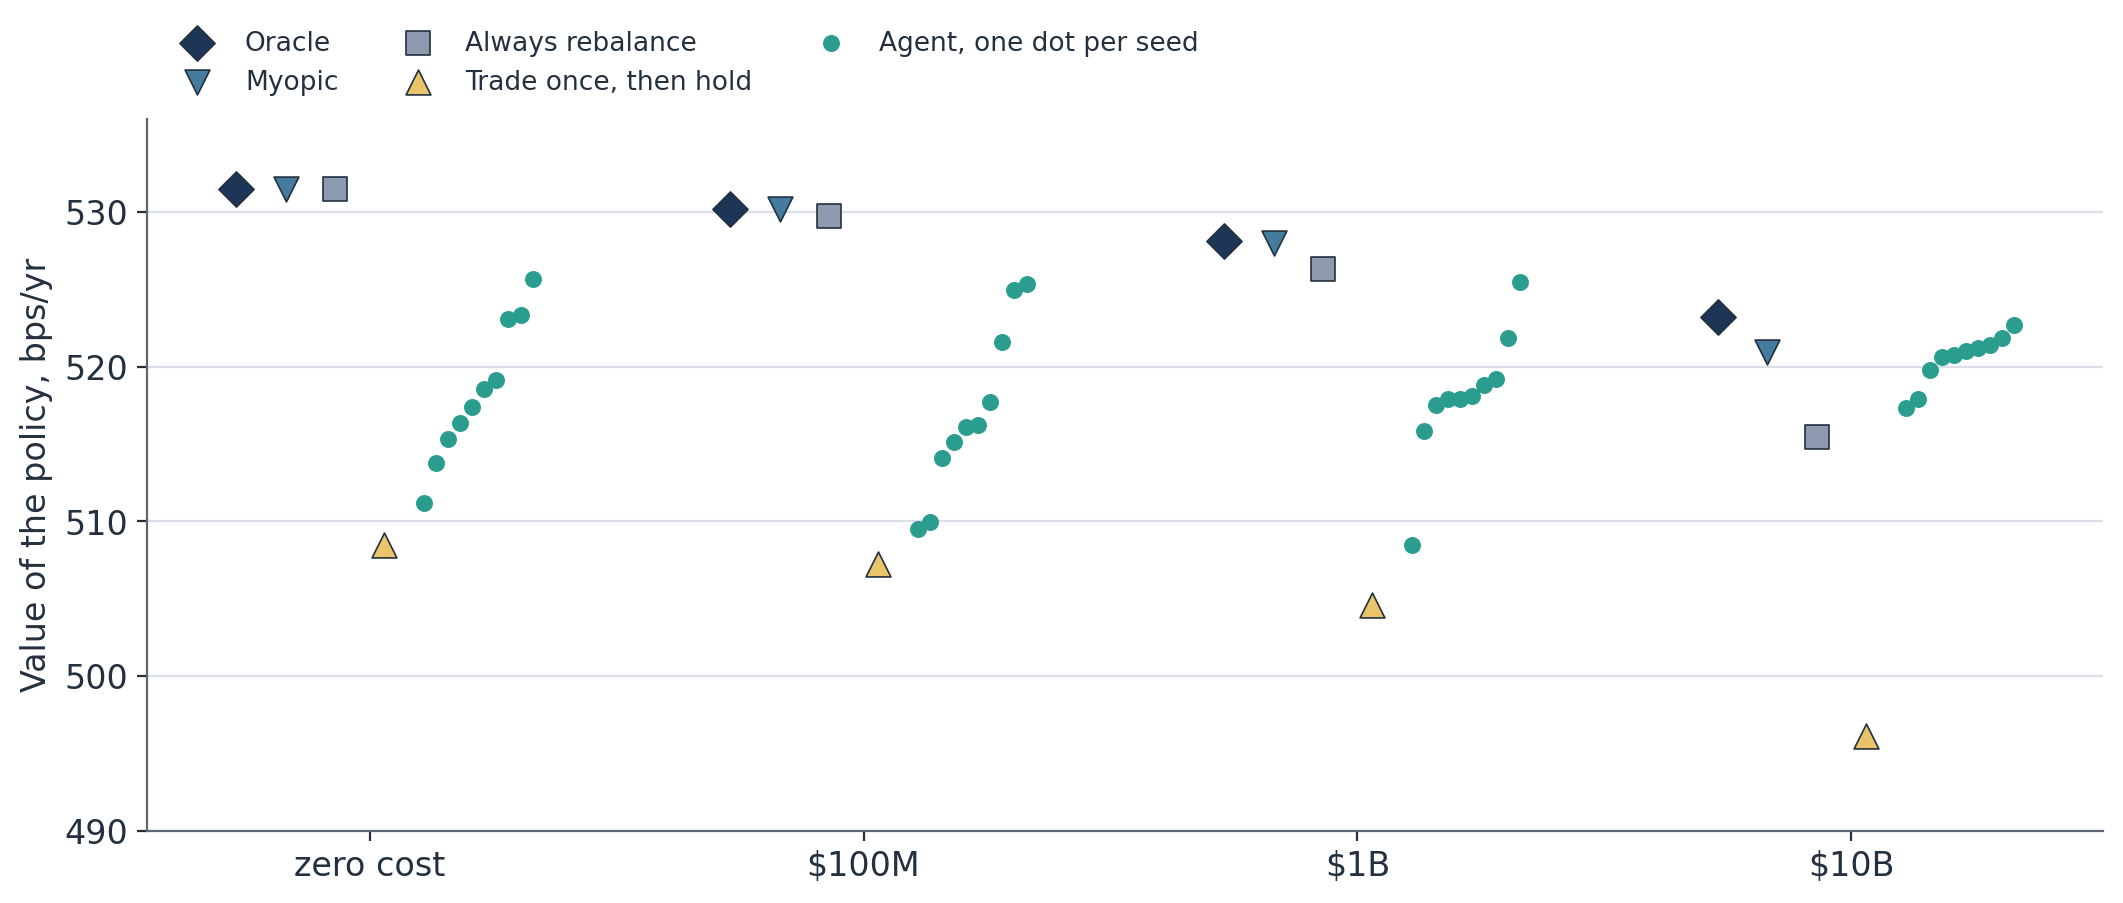
\includegraphics[keepaspectratio,alt={Figure A14. Redesign: value of each policy by cost level (Table 10), with every seed of the agent.}]{figures/fig_tc_values.png}}
\caption{\textbf{Figure A14.} Redesign: value of each policy by cost
level (Table 10), with every seed of the agent.}
\end{figure}

\begin{figure}
\centering
\pandocbounded{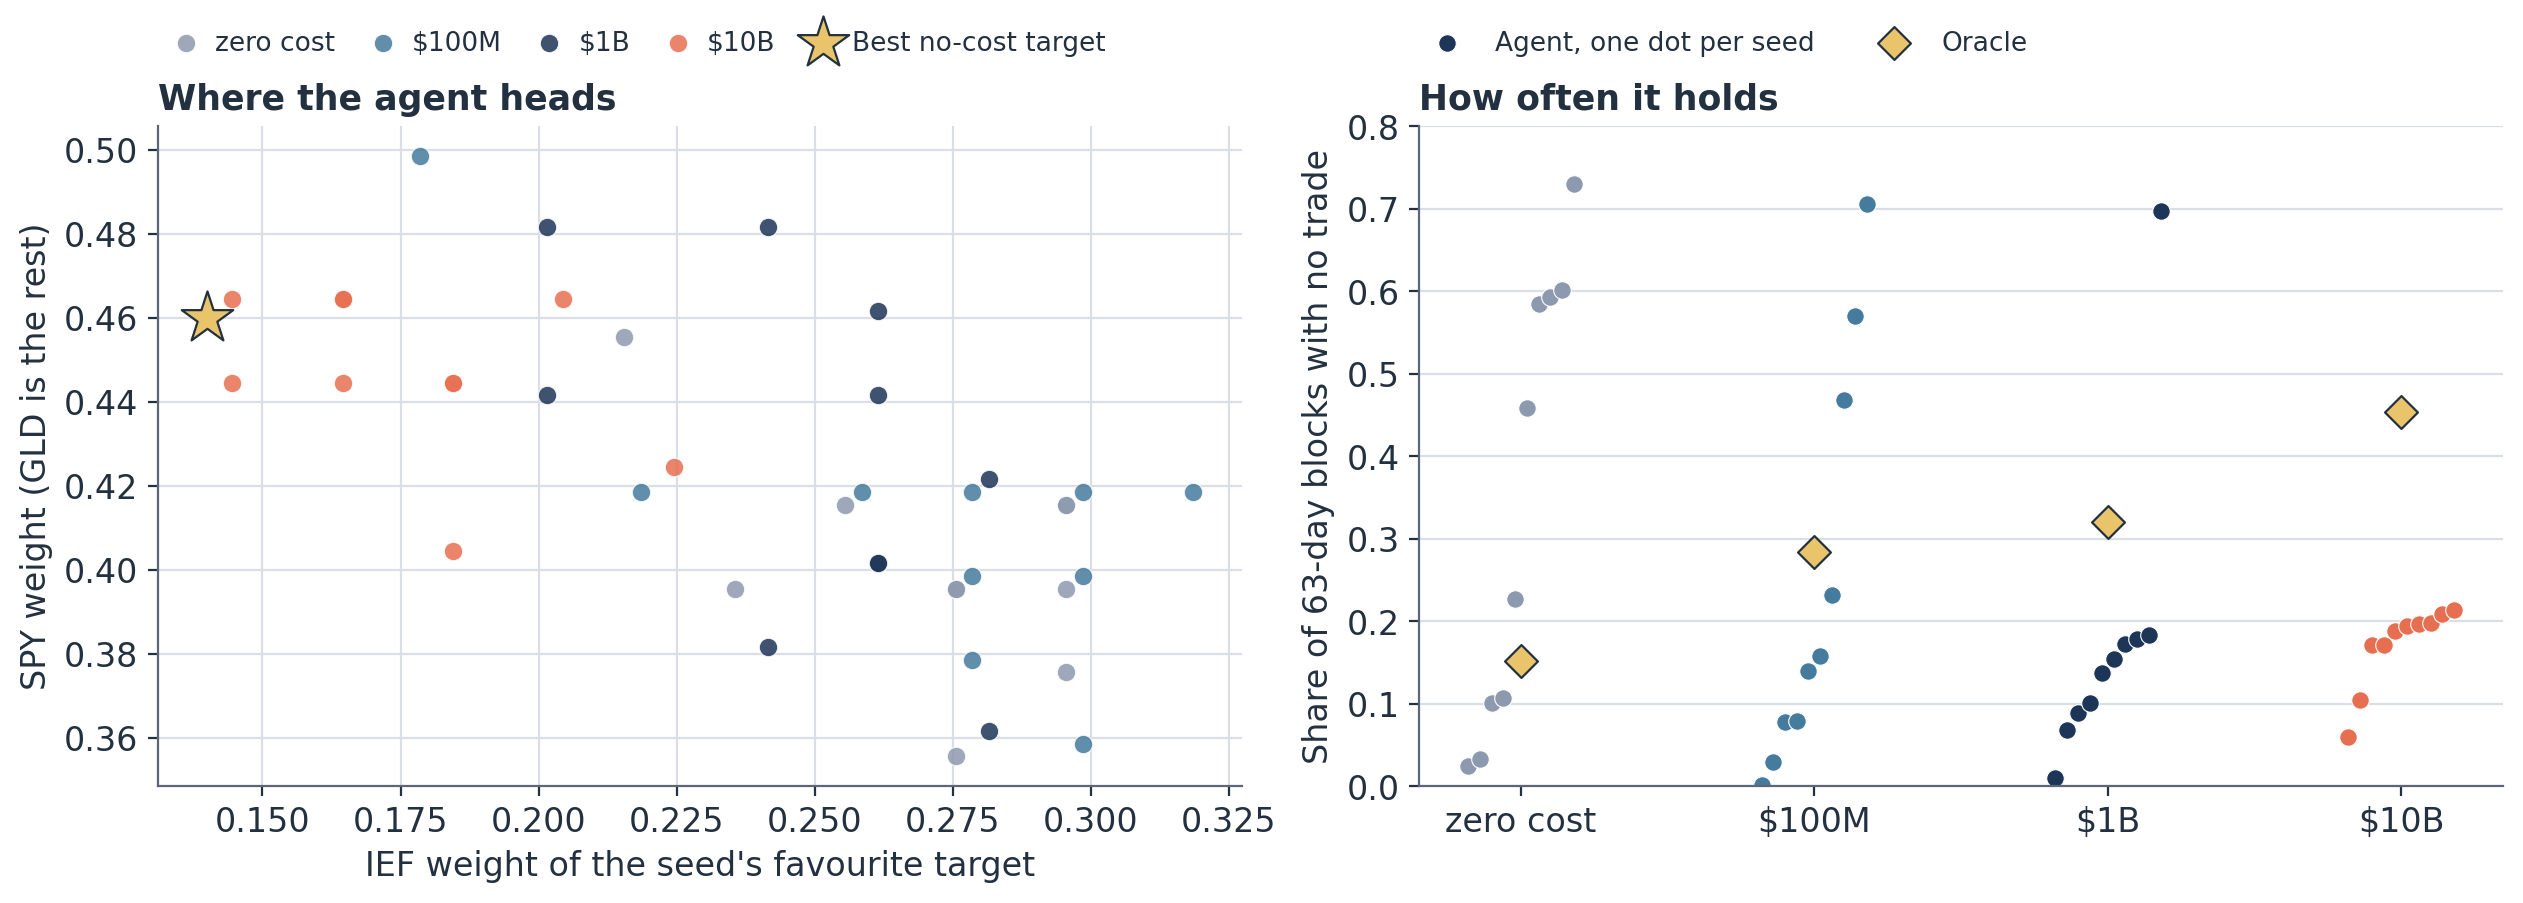
\includegraphics[keepaspectratio,alt={Figure A15. Left: each seed's favorite target. Right: the share of blocks in which the agent and the oracle do not trade.}]{figures/fig_tc_targets_hold.png}}
\caption{\textbf{Figure A15.} Left: each seed's favorite target. Right:
the share of blocks in which the agent and the oracle do not trade.}
\end{figure}

\begin{figure}
\centering
\pandocbounded{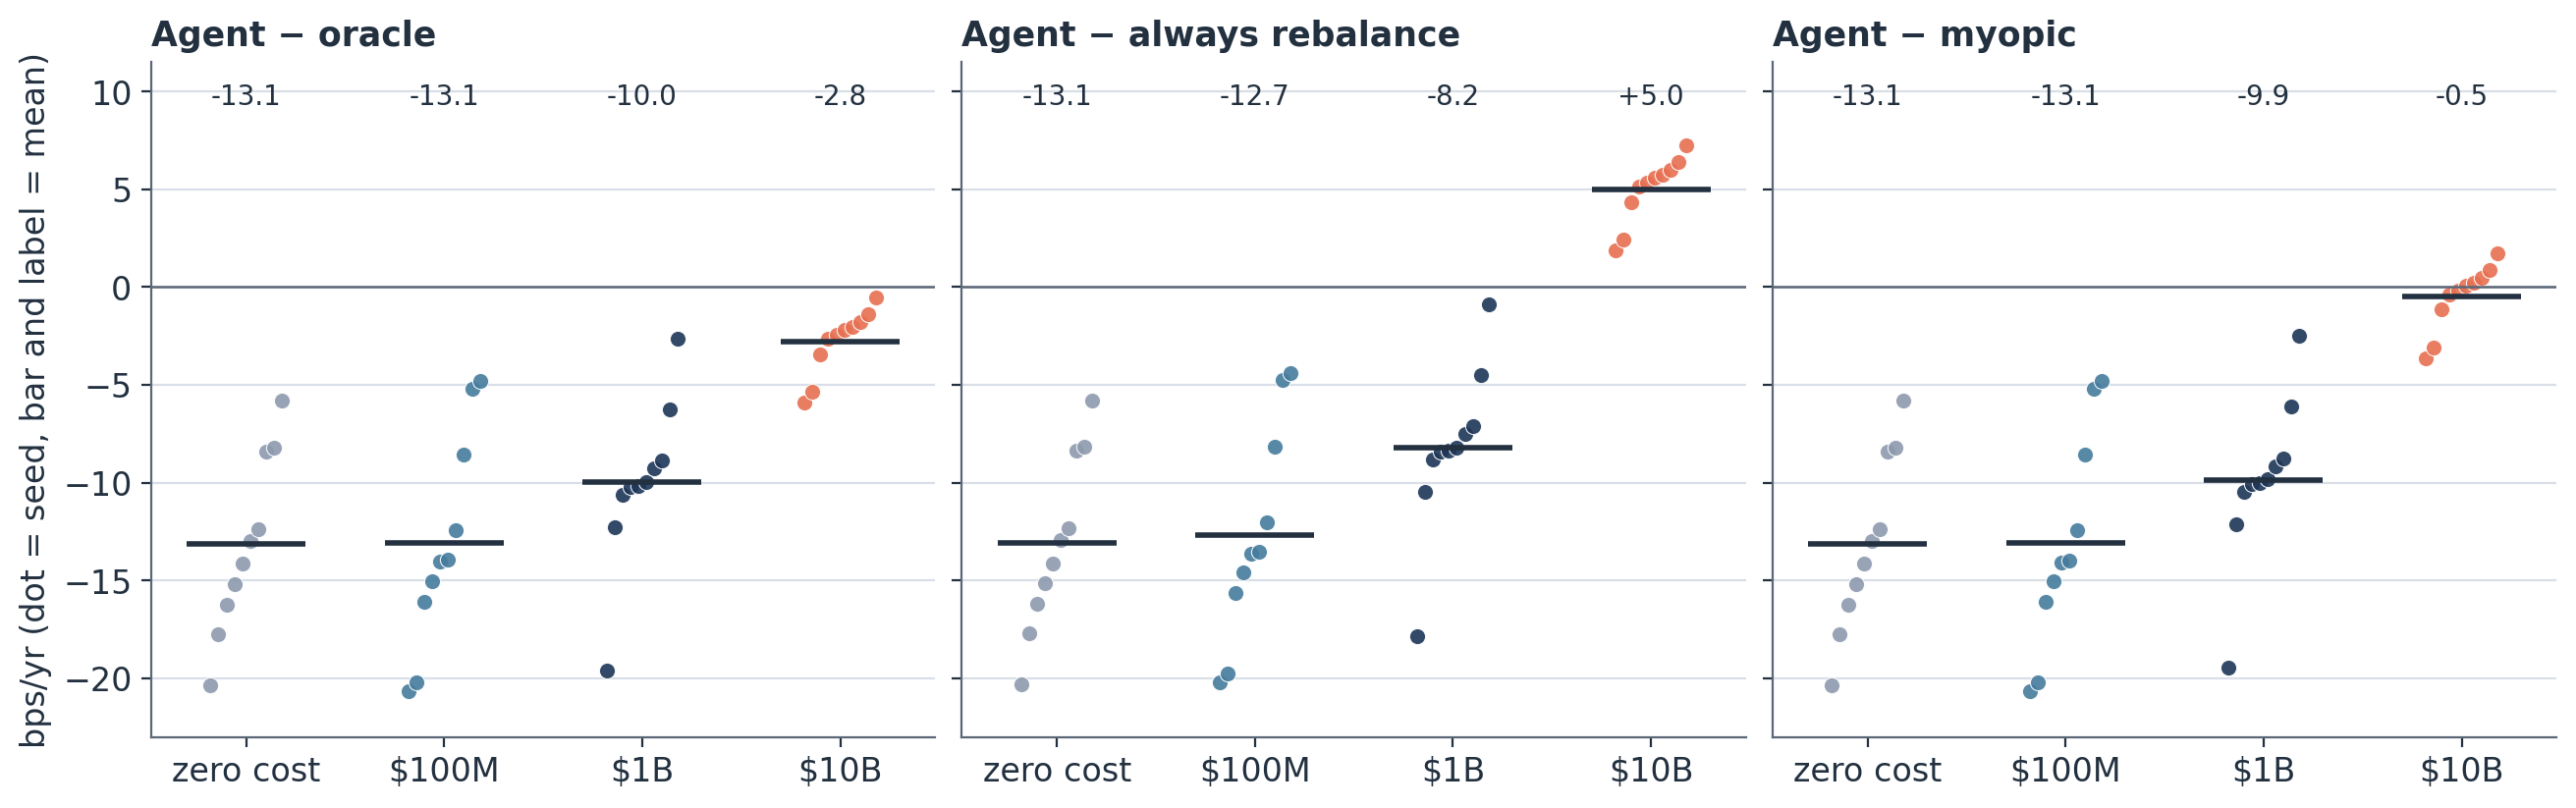
\includegraphics[keepaspectratio,alt={Figure A16. Every seed against the oracle, always rebalancing and the myopic policy.}]{figures/fig_tc_vs_references.png}}
\caption{\textbf{Figure A16.} Every seed against the oracle, always
rebalancing and the myopic policy.}
\end{figure}

\begin{figure}
\centering
\pandocbounded{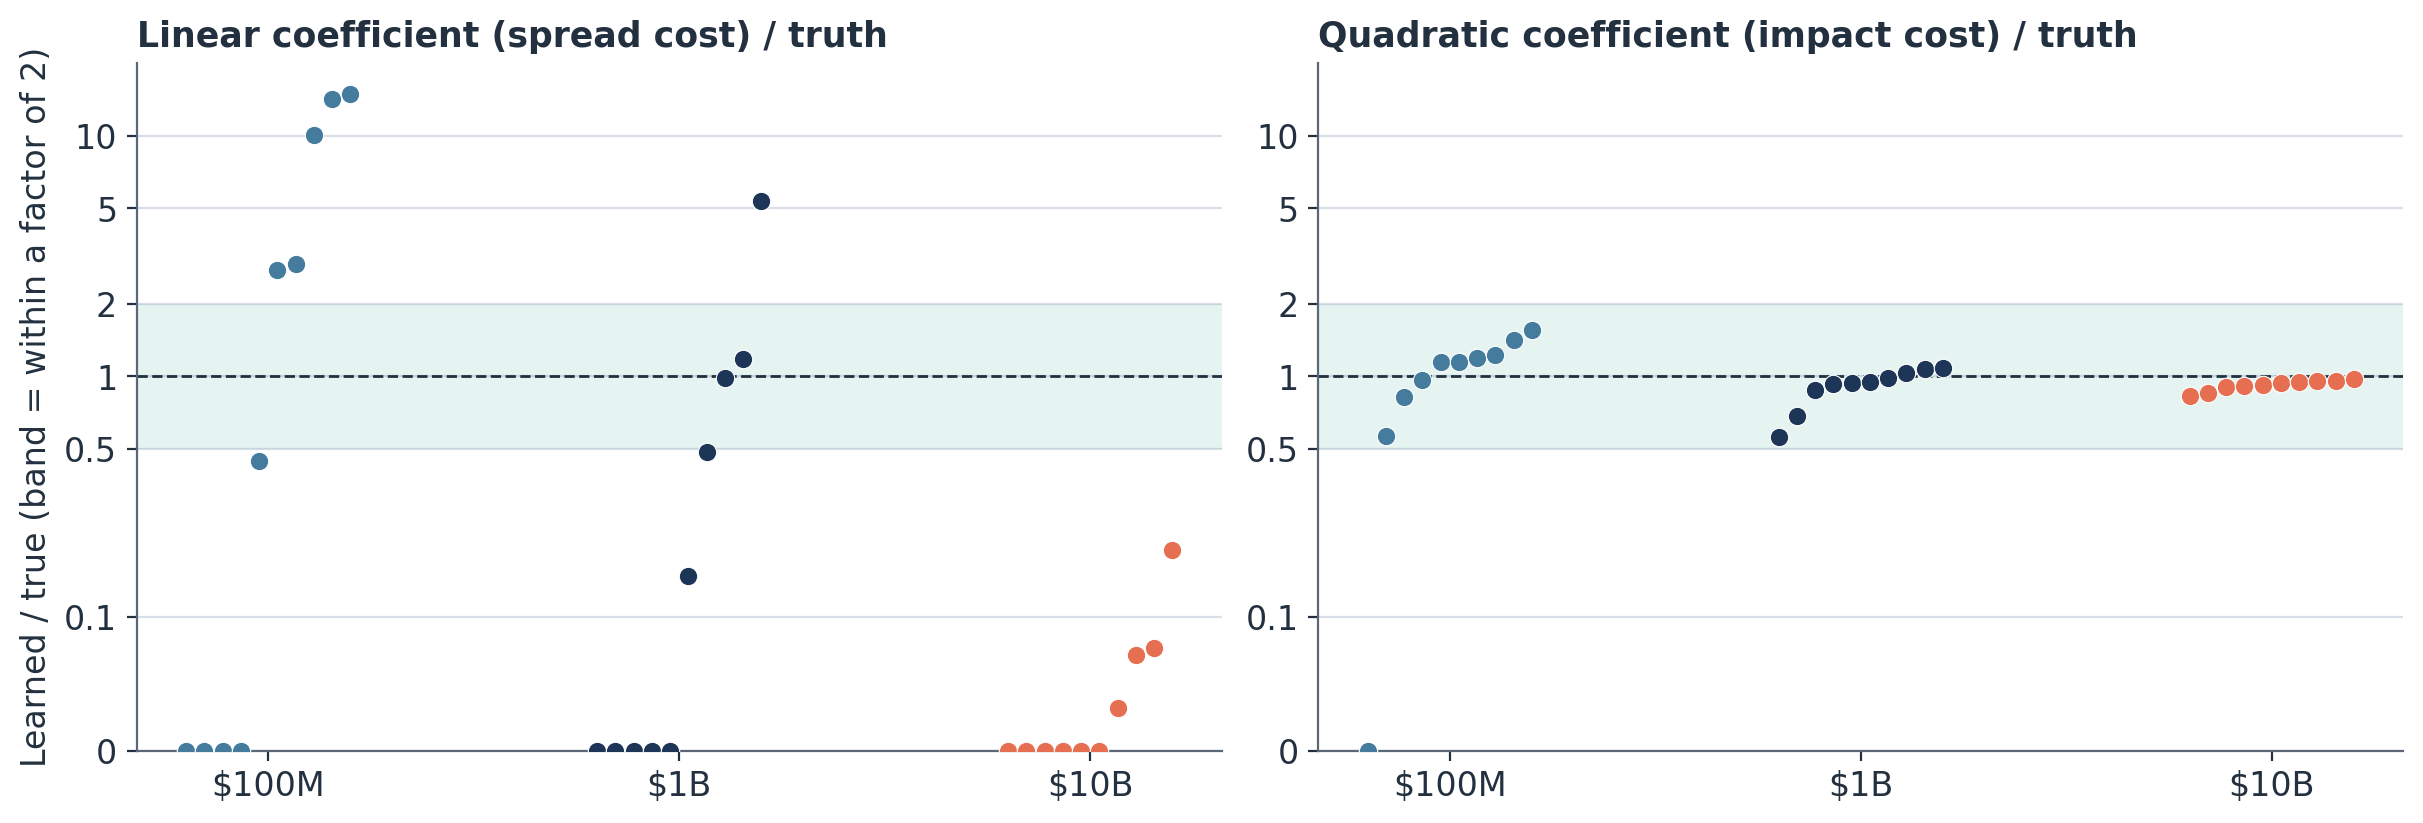
\includegraphics[keepaspectratio,alt={Figure A17. Final learned cost coefficients as a ratio to the truth, one dot per seed.}]{figures/fig_tc_costs.png}}
\caption{\textbf{Figure A17.} Final learned cost coefficients as a ratio
to the truth, one dot per seed.}
\end{figure}

\begin{table}[htbp]
\centering\small
\caption{\textbf{Table A3.} Expectations registered on 20 November 2026,
before any final transaction-cost run. Levels are in the order zero,
\$100M, \$1B, \$10B. Eight met, four partly met.}
\begin{tabular}{@{}
  >{\raggedright\arraybackslash}p{(\linewidth - 6\tabcolsep) * \real{0.0485}}
  >{\raggedright\arraybackslash}p{(\linewidth - 6\tabcolsep) * \real{0.4175}}
  >{\raggedright\arraybackslash}p{(\linewidth - 6\tabcolsep) * \real{0.4175}}
  >{\raggedright\arraybackslash}p{(\linewidth - 6\tabcolsep) * \real{0.1165}}@{}}
\toprule\noalign{}
\begin{minipage}[b]{\linewidth}\raggedright
\end{minipage} & \begin{minipage}[b]{\linewidth}\raggedright
Registered expectation
\end{minipage} & \begin{minipage}[b]{\linewidth}\raggedright
Result
\end{minipage} & \begin{minipage}[b]{\linewidth}\raggedright
Verdict
\end{minipage} \\
\midrule\noalign{}
E1 & Agent − oracle between −1 and −8 bps/yr at each level; negative on
at least 8 of 10 seeds & −13.1, −13.1, −10.0, −2.8; negative on 10 of 10
at every level & Partly met \\
E2 & The target error is most of the gap at zero, \$100M and \$1B &
Target −13.1, −12.8, −9.0 against timing 0.0, 0.1, 0.8 & Met \\
E3 & Agent loses to always rebalancing at \$100M and \$1B; relatively
better at \$10B & −12.7, −8.2; +5.0 at \$10B & Met \\
E4 & Timing value rises from \$1B to \$10B and is positive at \$10B;
within ±1 at zero and \$100M & 0.8 → 6.2; 0.0 and 0.1 & Met \\
E5 & Agent beats trade-once-then-hold at every level and seed & Lowest
seed 2.68, 2.30, 3.93, 21.19 & Met \\
E6 & Agent loses to myopic at every level & −13.1, −13.1, −9.9, −0.5. At
\$10B the mean (across-seed SE 0.54) is not distinguishable from zero,
and the agent beats myopic on 5 of 10 seeds & Met \\
E7 & Hold fraction varies across seeds; higher at \$10B than at zero; at
zero the agent holds more than the oracle & Spread 0.01 to 0.70 at \$1B;
0.35 against 0.15 at zero; mean at \$10B (0.17) is lower than at zero
(0.35) & Partly met \\
E8 & Quadratic coefficient within ×2 on at least 7 of 10 seeds at \$1B
and \$10B; linear coefficient off by more than ×2 on at least 3 of 10 &
Quadratic: 10 and 10. Linear off on 10, 8 and 10 of 10 at \$100M, \$1B,
\$10B & Met \\
E9 & Fewer than 5 of 10 seeds converge under the 20 November rule; none
under the two earlier rules & 5, 7, 7, 4; none under the earlier rules &
Partly met \\
E10 & Averaged and last-iterate policies differ by under 1 bps/yr &
−0.35, 0.42, 0.20, 0.13 & Met \\
E11 & Precision target missed at \$1B (SE 0.5 to 0.8), met at \$10B &
Missed at \$1B with SE 0.94; met at \$10B & Partly met \\
E12 & SD across seeds of agent − oracle at \$1B at least 0.5 & 4.32 &
Met \\
\bottomrule\noalign{}
\end{tabular}
\end{table}

\begin{table}[htbp]
\centering\small
\caption{\textbf{Table A4.} Absolute weight differences from the
continuous optimum \(w^*\) (SPY 0.4688, IEF 0.1363, GLD 0.3948) for
every seed at γ = 5 on the 20\% grid. EFA, EEM, VNQ and DBC are zero in
\(w^*\) and in every seed. The last column is the sum (L1
distance).}
\begin{tabular}{@{}lrrrrrr@{}}
\toprule\noalign{}
Seed & SPY & IEF & LQD & TIP & GLD & L1 \\
\midrule\noalign{}
0 & 0.069 & 0.064 & 0 & 0 & 0.005 & 0.138 \\
1 & 0.131 & 0.136 & 0 & 0 & 0.005 & 0.273 \\
2 & 0.069 & 0.264 & 0 & 0 & 0.195 & 0.527 \\
3 & 0.069 & 0.136 & 0 & 0.200 & 0.005 & 0.410 \\
4 & 0.069 & 0.136 & 0.200 & 0 & 0.005 & 0.410 \\
5 & 0.069 & 0.064 & 0 & 0 & 0.005 & 0.138 \\
6 & 0.131 & 0.136 & 0 & 0 & 0.005 & 0.273 \\
7 & 0.131 & 0.064 & 0 & 0 & 0.195 & 0.390 \\
8 & 0.069 & 0.064 & 0.200 & 0 & 0.195 & 0.527 \\
9 & 0.069 & 0.064 & 0 & 0 & 0.005 & 0.138 \\
\bottomrule\noalign{}
\end{tabular}
\end{table}

\clearpage

\subsection{Appendix B.
Reproducibility}\label{appendix-b.-reproducibility}

\textbf{Commands} (from the repository root; full instructions in
\texttt{README.md}).

\begin{verbatim}
python -m pytest src/tests -q                      # test suite
python -m src.data.clean                           # rebuild data/processed/ from committed raw data
python -m src.run_experiments --results-dir results/repro        # the four pre-registered experiments
python -m src.run_experiments --run b63 --results-dir results/b63   # a post hoc run (same pattern for the others)
python -m src.benchmarks.closed_form_table         # budget-only closed form, results/benchmarks/
python -m src.tc_drift.oracle_runs                 # transaction-cost oracle tables
python -m src.tc_drift.run all --workers 7         # 4 cost levels x 10 seeds, then scoring
python -m src.reporting.build --all                # per-run HTML reports
python -m src.transaction_costs experiments/transaction-costs/quadratic-cost.json   # first transaction-cost design
python -m src.tc_sweep_report                      # its report, reports/tc-quadratic-cost/
sh docs/report/build.sh                            # figures, LaTeX paper (REPORT.pdf), slides.html and .pdf
\end{verbatim}

\texttt{docs/report/build.sh} runs
\texttt{docs/report/figures/make\_figures.py} (every figure in the
report and the slides), converts \texttt{REPORT.md} to LaTeX with pandoc
(\texttt{latex/REPORT.tex}, with \texttt{latex/preamble.tex},
\texttt{latex/table\_captions.lua} and \texttt{latex/fix\_tables.py})
and typesets \texttt{REPORT.pdf} with XeLaTeX, then runs
\texttt{docs/report/slides/build\_slides.py} and prints
\texttt{slides.pdf}. Raw data must not be downloaded again; the
committed files, downloaded on 24 September 2026, are the calibration
source.

\textbf{Seeds.} Reported runs use master seed 20261016, split into
separate streams for training returns, the agent's exploration and
evaluation. Function-approximation step sizes were tuned on 20261103 and
the transaction-cost agent on 20261112.

\textbf{Run registry.}

{\def\LTcaptype{none} % do not increment counter
\begin{table}[htbp]
\centering\small
\begin{tabular}{@{}
  >{\raggedright\arraybackslash}p{(\linewidth - 6\tabcolsep) * \real{0.2500}}
  >{\raggedright\arraybackslash}p{(\linewidth - 6\tabcolsep) * \real{0.2500}}
  >{\raggedright\arraybackslash}p{(\linewidth - 6\tabcolsep) * \real{0.2500}}
  >{\raggedright\arraybackslash}p{(\linewidth - 6\tabcolsep) * \real{0.2500}}@{}}
\toprule\noalign{}
\begin{minipage}[b]{\linewidth}\raggedright
Run
\end{minipage} & \begin{minipage}[b]{\linewidth}\raggedright
Status
\end{minipage} & \begin{minipage}[b]{\linewidth}\raggedright
Date
\end{minipage} & \begin{minipage}[b]{\linewidth}\raggedright
Git reference
\end{minipage} \\
\midrule\noalign{}
Baseline: γ = 5 on 20\% and 25\% grids; γ = 3, 8 on 20\% &
Pre-registered (settings in \texttt{07bfb64}, 16 October) & 22 October &
tag \texttt{baseline-v1}; trained at \texttt{80a6e9c} \\
\texttt{eps-decay}, \texttt{b63} & Post hoc, registered 27 October & 28
October & tags \texttt{eps-decay}, \texttt{b63} \\
\texttt{n26m}, \texttt{all-three} & Post hoc, registered 27 October & 28
October & \texttt{81814e6} \\
\texttt{grid10-robustness} & Post hoc, registered 27 October & 29
October & \texttt{e13a9a6} \\
\texttt{tabular-const}, \texttt{fa-quadratic} & Post hoc, registered 5
November & 6 November & tags of the same names \\
\texttt{fa-spline} & Post hoc, registered 5 November & 6 November &
\texttt{bc311a3} \\
\texttt{fa-spline-grid10-eps3}, \texttt{-eps10} & Post hoc, registered
11 November & 11 November & \texttt{c0e5494} \\
First transaction-cost design & Post hoc & 6 November &
\texttt{da2b0fa} \\
Transaction costs with drift, 40 runs & Post hoc, expectations
registered 20 November & 20 November & \texttt{1787f0d}, clean tree \\
\bottomrule\noalign{}
\end{tabular}
\end{table}
}

\textbf{Versions.} Python 3.13.9, numpy 2.3.5, scipy 1.16.3, pandas
2.3.3, matplotlib 3.10.6, yfinance 1.7.0. The transaction-cost runs used
one BLAS thread on an arm64 Mac.

\subsection{Appendix C. Disclosures for the transaction-cost
extension}\label{appendix-c.-disclosures-for-the-transaction-cost-extension}

The forty runs are post hoc relative to the baseline and came from
commit \texttt{1787f0d} with a clean working tree. Benchmark information
entered the design in several ways, none of which reaches the agent
during training.

\begin{enumerate}
\def\labelenumi{\arabic{enumi}.}
\tightlist
\item
  The three-ETF universe is the support of the nine-asset optimum.
\item
  The cost levels were chosen with the oracle's results in view,
  although κ and λ themselves come from our liquidity data.
\item
  The two cost features build in the functional form of the cost; the
  agent learns two coefficients, constrained to be nonnegative.
\item
  The learning rule, the parameter averaging and the convergence rule
  were chosen with pilot diagnostics that used the benchmark; the
  convergence rule changed three times before it was frozen on 20
  November, and under the earlier versions applied to the last iterate
  no seed converges at any level.
\item
  The convergence check reads the policy at checkpoints, so a switch
  that reverts between checkpoints goes unseen.
\item
  Tuning used the \$1 billion level only, and a first set of six pilot
  runs was discarded.
\item
  The always-rebalance and trade-once references use the best no-cost
  target, computed from μ and Σ.
\item
  One cost applies to every asset pair, which undercharges the typical
  SPY-against-GLD trade by about a fifth.
\item
  The oracle summary and the tuning records were produced from code with
  uncommitted changes; the final agent runs were not.
\item
  Our precision target at \$1 billion was missed: the paired standard
  error of one seed's gap is 0.94 bps/yr against a target of 0.59.
\item
  Drift is applied to excess returns, with an effect bounded at 7.1 ×
  10⁻⁶.
\item
  One of the oracle's verification checks was restated after the fact,
  and another is a two-standard-error bound.
\item
  The twelve registered expectations (Table A3) lean on the \$1 billion
  tuning pilot, three runs of the same agent on a different master seed,
  and on that pilot's benchmark diagnostics (oracle gaps, the favorite
  target's utility loss, the true cost coefficients). They are informed
  by benchmark information about the same agent on other seeds, and were
  frozen on 20 November before any final run.
\end{enumerate}

\end{document}
